\documentclass[letterpaper]{sig-alternate-10pt}

%%%%%%%%%%%%%%%%%%%%%%%%%%%%%%%%%%%%%%%%%%%%%%%%%%%%%%%%%%%%%%%%%%%%%%%%%%%%%%%%
\usepackage{color}
\usepackage{cite}
\usepackage{multirow}
\usepackage{xspace}

\newcommand{\fixme}[1]{{\textcolor{red}{[FIXME: #1]}}}
\newcounter{mynote}[section]
\newcommand{\notecolor}{blue}
\newcommand{\thenote}{\thesection.\arabic{mynote}}
\newcommand{\aditya}[1]{\refstepcounter{mynote}{\bf \textcolor{\notecolor}{$\ll$AA~\thenote: {\sf #1}$\gg$}}}
\newcommand{\li}[1]{\refstepcounter{mynote}{\bf \textcolor{\notecolor}{$\ll$LEL~\thenote: {\sf #1}$\gg$}}}
\newcommand{\tnote}[1]{\refstepcounter{mynote}{\bf \textcolor{\notecolor}{$\ll$TCR~\thenote: {\sf #1}$\gg$}}}
\newcommand{\keqhe}[1]{\refstepcounter{mynote}{\bf \textcolor{\notecolor}{$\ll$HE~\thenote: {\sf #1}$\gg$}}}
\newcommand{\marina}[1]{\refstepcounter{mynote}{\bf \textcolor{\notecolor}{$\ll$MT~\thenote: {\sf #1}$\gg$}}}
\newcommand{\junaid}[1]{\refstepcounter{mynote}{\bf \textcolor{\notecolor}{$\ll$JK~\thenote: {\sf #1}$\gg$}}}
\newcommand{\sourav}[1]{\refstepcounter{mynote}{\bf \textcolor{\notecolor}{$\ll$SD~\thenote: {\sf #1}$\gg$}}}
\newcommand{\anote}[1]{\refstepcounter{mynote}{\bf \textcolor{\notecolor}{$\ll$AEF~\thenote: {\sf #1}$\gg$}}}
\newcommand{\aaron}[1]{\refstepcounter{mynote}{\bf
\textcolor{\notecolor}{$\ll$AGJ: {\sf #1}$\gg$}}}
\renewcommand{\aditya}[1]{}
%\renewcommand{\aaron}[1]{}
\renewcommand{\keqhe}[1]{}
\renewcommand{\sourav}[1]{}


\newcommand{\pollstats}[1]{{pollstats }}
\newcommand{\packetin}{{\em packet\_in}\xspace}
\newcommand{\packetout}{{\em packet\_out}\xspace}
\newcommand{\flowmod}{{\em flow\_mod}\xspace}
\newcommand{\polling}[1]{{flow statistics polling}}


\newcommand{\Broadcom}{Broadcom\xspace}
\newcommand{\BroadcomOne}{BCM-1.0\xspace}
\newcommand{\BroadcomThree}{BCM-1.3\xspace}
\newcommand{\Intel}{Intel\xspace}
\newcommand{\IBM}{IBM\xspace}
\newcommand{\numVendors}{three\xspace}
\newcommand{\numCombos}{four\xspace}

\newcommand{\FE}{FE\xspace}
\newcommand{\RR}{RR\xspace}
\newcommand{\RO}{RO\xspace}

\newcommand{\tabref}[1]{{Table~\ref{#1}}}
\newcommand{\figref}[1]{{Figure~\ref{#1}}}
\newcommand{\figsref}[2]{{Figure~\ref{#1} and \ref{#2}}}
\newcommand{\algref}[1]{{Algorithm~\ref{#1}}}
\newcommand{\secref}[1]{{\S\ref{#1}}}
\newcommand{\appref}[1]{{Appendix~\ref{#1}}}
%\newcommand{\tabincell}[2]{\begin{tabular}{@{}#1@{}}#2\end{tabular}}

\newenvironment{compactitemize}
{
    \begin{itemize}
    \vspace{-1ex}
    \setlength{\topsep}{0pt}
    \setlength{\itemsep}{0em}
    \setlength{\parskip}{0pt}
    \setlength{\parsep}{0pt}
}
{
    \vspace{-1ex}
    \end{itemize}
}


\newcommand{\headingg}[1]{\noindent{\textit{#1}}}
\newcommand{\bheadingg}[1]{\noindent{\textbf{#1}}}
\newcommand{\bheading}[1]{{\vspace{4pt}\noindent\textbf{#1}}}
\newcommand{\minisection}[1]{\noindent{{\bf #1.}}}

\newcommand{\compactcaption}[1]{\vspace{-1em}\caption{#1}\vspace{-1em}}
\newcommand{\botcompactcaption}[1]{\vspace{-0.5em}\caption{#1}\vspace{-1em}}
\newcommand{\topcompactcaption}[1]{\vspace{-1em}\caption{#1}\vspace{-0.5em}}
%\renewcommand{\compactcaption}[1]{\caption{#1}}
%\renewcommand{\botcompactcaption}[1]{\caption{#1}}
%\renewcommand{\topcompactcaption}[1]{\caption{#1}}

\newcommand{\tabincell}[2]{\begin{tabular}{@{}#1@{}}#2\end{tabular}}

% ========================================================================
% Lists

\newlength{\saveparindent}
\setlength{\saveparindent}{\parindent}
\newlength{\saveparskip}
\setlength{\saveparskip}{\parskip}

\newcounter{ctr}
\newcounter{savectr}
\newcounter{ectr}

\newenvironment{newitemize}{%
\begin{list}{$\bullet$}{\labelwidth=9pt%
\labelsep=7pt \leftmargin=16pt \topsep=1pt%
\setlength{\listparindent}{\saveparindent}%
\setlength{\parsep}{\saveparskip}%
\setlength{\itemsep}{1pt} }}{\end{list}}

\newenvironment{newenum}{%
\begin{list}{{\rm (\arabic{ctr})}\hfill}{\usecounter{ctr} \labelwidth=18pt%
\labelsep=7pt \leftmargin=25pt \topsep=3pt%
\setlength{\listparindent}{\saveparindent}%
\setlength{\parsep}{\saveparskip}%
\setlength{\itemsep}{2pt} }}{\end{list}}

\newenvironment{tiret}{%
\begin{list}{\hspace{2pt}\rule[0.5ex]{6pt}{1pt}\hfill}{\labelwidth=15pt%
\labelsep=3pt \leftmargin=22pt \topsep=4pt%
\setlength{\listparindent}{\saveparindent}%
\setlength{\parsep}{\saveparskip}%
\setlength{\itemsep}{4pt}}}{\end{list}}

\newenvironment{bigtiret}{%
\begin{list}{\hspace{2pt}\rule[0.5ex]{6pt}{1pt}\hfill}{\labelwidth=15pt%
\labelsep=3pt \leftmargin=22pt \topsep=10pt%
\setlength{\listparindent}{\saveparindent}%
\setlength{\parsep}{\saveparskip}%
\setlength{\itemsep}{10pt}}}{\end{list}}

\newenvironment{bigblock}{%
\begin{list}{\hfill}{\labelwidth=0pt%
\labelsep=0pt \leftmargin=0pt \topsep=6pt%
\setlength{\listparindent}{\saveparindent}%
\setlength{\parsep}{\saveparskip}%
\setlength{\itemsep}{6pt}}}{\end{list}}

\newenvironment{blocklist}{\begin{list}{}{\labelwidth=0pt%
\labelsep=0pt \leftmargin=0pt \topsep=10pt%
\setlength{\listparindent}{\saveparindent}%
\setlength{\parsep}{\saveparskip}%
\setlength{\itemsep}{20pt}}}{\end{list}}

\newenvironment{blocklistindented}{\begin{list}{}{\labelwidth=0pt%
\labelsep=25pt \leftmargin=25pt\topsep=2pt%
\setlength{\listparindent}{\saveparindent}%
\setlength{\parsep}{\saveparskip}%
\setlength{\itemsep}{2pt}}}{\end{list}}

\newenvironment{onelist}{%
\begin{list}{\textbf{\arabic{ctr}.}\hfill}{\usecounter{ctr} \labelwidth=16pt%
\labelsep=5pt \leftmargin=21pt \topsep=5pt%
\setlength{\listparindent}{\saveparindent}%
\setlength{\parsep}{\saveparskip}%
\setlength{\itemsep}{5pt}}}{\end{list}}

\newenvironment{twolist}{%
\begin{list}{{\rm (\arabic{ctr}.\arabic{ectr})}%
\hfill}{\usecounter{ectr} \labelwidth=26pt%
\labelsep=7pt \leftmargin=33pt \topsep=2pt%
\setlength{\listparindent}{\saveparindent}%
\setlength{\parsep}{\saveparskip}%
\setlength{\itemsep}{2pt} }}{\end{list}}

\newenvironment{collist}{%
\begin{list}{{\rm (\arabic{ctr}.\arabic{ectr})}%
\hfill}{\usecounter{ectr} \labelwidth=26pt%
\labelsep=7pt \leftmargin=33pt \topsep=3pt%
\setlength{\listparindent}{\saveparindent}%
\setlength{\parsep}{\saveparskip}%
\setlength{\itemsep}{3pt} }}{\end{list}}

\newenvironment{centerlist}{%
\begin{list}{\mbox{}}{\labelwidth=0pt%
\labelsep=0pt \leftmargin=0pt \topsep=1pt%
\setlength{\listparindent}{\saveparindent}%
\setlength{\parsep}{\saveparskip}%
\setlength{\itemsep}{1pt} }}{\end{list}}

\newenvironment{newcenter}[1]{\begin{centerlist}\centering%
\item #1}{\end{centerlist}}

% =========================================================================

\newcommand{\calX}{{\mathcal X}}
\newcommand{\Colon}{{:\:}}
 
\usepackage{times}
\usepackage{subfig}
\usepackage{graphicx}
\usepackage{xcolor}
\usepackage{url,caption}
\usepackage{epstopdf}
\usepackage[]{algorithm2e}
\usepackage{algorithmic}
\usepackage{mathtools}
\usepackage[titletoc]{appendix}
\usepackage{fontenc}
\usepackage[utf8]{inputenc}
\DeclarePairedDelimiter{\abs}{\lvert}{\rvert}
%\usepackage[font={small}]{caption}
%\usepackage[section] {placeins}
%% Define a new 'leo' style for the package that will use a smaller font.
\makeatletter
\def\url@leostyle{%
  \@ifundefined{selectfont}{\def\UrlFont{\sf}}{\def\UrlFont{\small\ttfamily}}}
\makeatother
%% Now actually use the newly defined style.
\urlstyle{leo}
%\makeatletter
%\def\@copyrightspace{\relax}
%\makeatother
\newcommand{\Tabs}{
  xx\= xx\= xx\= xx\= xx\= xx\= xx\= xx\=xx\= xx\= xx\= xx\=\kill}

\newenvironment{program}[3]{
  \begin{figure}[hbtp]
    \begin{center}
    \fbox{
      {\small % yry
      \begin{minipage}{\textwidth}
      \begin{tabbing}
      \Tabs
      #3
      \end{tabbing}
      \vspace{-0.25in}
      \end{minipage}
      } % yry
    \vspace{-0.15in}
    }
    \end{center}
    \vspace{-0.2in}
    \caption{\label{#1} #2}
    \vspace{-0.1in}
  \end{figure}}{}

\begin{document}
%\title{Mazu: Taming Long tail Latency \\in Software Defined Networks}
%\title{Mazu: Taming Latency in Software Defined Networks}
%\title{Latency in Software Defined Networks: \\Measurements and Mitigation Techniques}

\title{Measuring Control Plane Latency in SDN-enabled Switches}
%\author{Paper \#91, 12 pages + 1 page appendix}

%\numberofauthors{1}
\author{
{
    Keqiang He$^\dag$,
    Junaid Khalid$^\dag$,
    Aaron Gember-Jacobson$^\dag$,
    Sourav Das$^\dag$,
    Chaithan Prakash$^\dag$,
}\\
{
    Aditya Akella$^\dag$,
    Li Erran Li*,
    Marina Thottan*
}\\
{\em $^\dag$University of Wisconsin-Madison, *Bell Labs}
}
\maketitle

\begin{abstract}

Datacenter networks deal with a variety of workloads, 
ranging from latency-sensitive small flows to bandwidth-hungry large flows. 
Load balancing schemes based on flow hashing, \eg{}, ECMP, cause congestion 
when hash collisions occur and can perform poorly in asymmetric topologies. 
Recent proposals to load balance the network require centralized traffic engineering, multipath-aware
transport, or expensive specialized hardware.
We propose a mechanism that avoids these limitations by (i) pushing
load-balancing functionality into the soft network edge (\eg{},
virtual switches) such that no changes are required in the transport
layer, customer VMs, or networking hardware, and (ii) load balancing
on fine-grained, near-uniform units of data (flowcells) that fit
within end-host segment offload optimizations used to support fast
networking speeds.
We design and implement such a soft-edge load balancing scheme, called
Presto, and evaluate it on a 10 Gbps physical testbed.
We demonstrate the computational impact of packet reordering on
receivers and propose a mechanism to handle reordering in the TCP receive
offload functionality.
Presto's performance closely tracks that of a single, non-blocking
switch over many workloads and is adaptive to
failures and topology asymmetry.

\iffalse
Datacenter networks must deal with a variety of workloads,
ranging from latency-sensitive small flows to bandwidth-hungry large flows.
Flow hashing load balancing schemes, e.g. ECMP, cause congestion
when hash collisions occur and perform poorly in asymmetric topologies.
Recent proposals to effectively load balance the network require multipath-aware transport, 
centralized traffic engineering or expensive specialized hardware. Our scheme 
overcomes these limitations by (i) pushing load-balancing functionality into 
the emerging soft network edge (e.g. virtual switches) such that no changes 
are required in the transport layer, customer VMs, or networking hardware, 
and (ii) load balancing on fine-grained, near-uniform units of data that 
naturally fit within end-host segment offload optimizations used to support 
fast networking speeds
and near-optimally load balance over symmetric network topologies.
We uncover the problems of fine-grained load balancing on packet reordering and 
propose a scheme to handle 
them in TCP receive offload funtionality without touching transport.
We design and implement a soft-edge load balancing scheme and evaluate it on a real 
10G testbed. 
Its performance tracks the performance of a 
single, non-blocking switch over many workloads (including trace driven) 
and is adaptive to failures and topology asymmetry.
\fi

\end{abstract}

\section{Introduction}\label{sec-intro}

Software defined networking (SDN) advocates for the separation of control and
data planes in network devices, and provides a logically centralized platform
to program data plane state~\cite{openflow,rethinking}.  This has opened the
door to rich network control applications that can adapt to changes in
network topology or traffic patterns more flexibly and more quickly than 
legacy control
planes~\cite{swan,b4,ananta,simple,elastictree,softcell,zupdate,microte}.



%However, many important management applications in these domains, such
%as fast fail-over, reactive routing of latency-sensitive flows, and
%fine-grained DC traffic engineering~\cite{microte}, are stretching SDN's
%capabilities. These applications require the ability to reprogram data plane
%state at very fine time-scales to optimally meet their objectives.
In order to optimally satisfy network objectives, many important control 
applications require the ability to reprogram data plane state at very fine 
time-scales. For instance, fine-grained data center
traffic engineering requires routes to be set up within a few hundred
milliseconds to leverage short-term traffic
predictability~\cite{microte}. Similarly, setting up routes in
cellular networks (when a device becomes active, or during a handoff)
must complete within $\sim$30-40ms to ensure users can interact with
Web services in a timely fashion~\cite{softcell}.
%  It is important that SDN support such
% applications, otherwise operators will be forced to adopt expensive custom
% solutions alongside SDN (e.g., bandwidth reservation, custom
% hardware/protocols, etc.), which can undermine SDN's ``CapEx'' and ``OpEx''
% benefits.  \aaron{Should the preceding sentence be cut, because the proxy
% seems like ``custom hardware''?}

For such applications, timely interaction between the logically
central SDN control plane and network switches is crucial. Timeliness
is determined by: (1) the speed of control programs, (2) the latency
to/from the logically central controller, and (3) the responsiveness
of network switches in interacting with the controller---specifically,
in generating the necessary input messages for control programs, and
in modifying forwarding state as dictated by them. Robust control
software design and advances in distributed controllers~\cite{onix}
have helped overcome the first two issues. However, with the focus in
current/upcoming generations of SDN switches being on the flexibility
benefits of SDN w.r.t. legacy technology, the third issue has
not gained much attention. Thus, it is unknown whether SDN can
provide sufficiently responsive control to support the aforementioned
applications.


% Alarmingly, preliminary studies~\cite{ucsdpaper,oflops} and anecdotal
% evidence suggest that the latencies of switch control actions (\#3
% above) are significant. However, it is unclear what factors impact
% these latencies, what the underlying causes are, and whether the
% causes are fundamental to switch designs. 

To this end, we present a thorough systematic exploration of latencies in 
%\#3 above in 
three types of production SDN switches from
\numVendors different vendors---Broadcom and Intel---using a variety
of workloads. We investigate the relationship between switch design
and observed latencies using both greybox probes and feedback from
vendors. Key highlights from our measurements are as follows: (1) We
find that {\em inbound latency}, i.e., the latency involved in the
switch generating events (e.g., when a flow is seen for the first
time) can be high (8 ms per packet on average on Intel). We find the
delay is particularly high whenever the switch is simultaneously
processing forwarding rules received from the controller. (2) We find
that {\em outbound latency}, i.e., the latency involved in the switch
installing/modifying/deleting forwarding rules provided by control
applications, is high as well (3ms and 30ms per rule for insertion and
modification, respectively, in Broadcom). The latency crucially
depends on the priority patterns both in rules being inserted as well as
those already in a switch's table. We find that there are significant
differences in latency trends across the three switches, pointing to
different internal optimizations.


Wouldn't improvements in switch designs eliminate these latencies over
time? Some of our findings show that poor switch software design
contributes significantly to observed latencies
(affirming~\cite{ucsdpaper,oflops}). We believe that near term work
will address these issues; our measurements with an early release of
Broadcom's OpenFlow 1.3 software exemplify this.

More crucially, our measurements also reveal latencies that appear to
be fundamentally rooted in hardware design: e.g., rules must be
organized in switch hardware tables in priority order, and
simultaneous switch control actions must contend for limited bus
bandwidth between a switch's CPU and ASIC. Unless the hardware
significantly changes---and our first-of-a-kind in-depth measurement
study may engender such changes---we believe these latencies will
manifest even in next generation switches.

%Our measurements point out to switch manufacturers and chip developers the
%steps they need to take to eliminate these latencies. 

%We find that poor switch software design contributes significantly to the
%observed high latencies. However, pathological interactions between some rule
%priority input sequences and switch hardware table  heuristics for rule
%layout play a significant  role in inflating latency as well.  Crucially, the
%latter issue is  fundamental and may be hard to overcome.

%Informed by our measurements, we design a framework called Mazu that {\em
%leverages} the centralized view and global control in SDN to overcome or
%mitigate the impact of latencies, including both latencies from
%implementation-related causes and those from fundamental ones.

Since hardware upgrade cycles are 5+ years long (according to anecdotal
evidence), operators need immediately deployable solutions to 
mitigate these latencies while they wait for switch software and hardware to
appropriately evolve. To this end, we design a framework called {\em Mazu}
that leverages SDN's central view and global control.  To mitigate inbound
latency arising from bus bottlenecks in switches,
%arising from data plane packet arrivals, 
Mazu redirects relevant packets to a fast proxy that generates the 
necessary messages for the controller.
%  By
% using a commodity machine, with high NIC-to-CPU bandwidth and a fast
% CPU, we are able to
This virtually eliminates inbound latency and saves
switch resources for rule updates.
%By leveraging a fast commodity processor and decoupling inbound and outbound
%actions, this eliminates inbound latency.

To mitigate outbound latency, which is intrinsically linked to switch
design (especially hardware),
% due to its intrinsic relation to switch software and hardware
we propose three techniques: {\em Flow
  engineering} (FE) leverages our empirical latency models to compute
paths such that the latency of installing forwarding state at any
switch is minimized. {\em Rule
  offloading} (RO) computes strategies for opportunistically
offloading installations of some forwarding state to downstream switches.
Finally, {\em rule reordering} (RR) sends rule installation
requests in an order that is optimal for the switch in question. By reducing
installation latency per switch (FE + RR) and enabling network-wide parallel updates (RO), 
rule updates can finish much faster, and the impact of
outbound latency is minimized.

 We evaluate these techniques for fast fail-over and responsive
 traffic engineering applications under various settings. Depending on
 the topology and the nature of rules in switches, we find that
in/outbound latencies can render SDN incapable of supporting such
applications. In contrast, 
our techniques can
 improve the time taken to update network state in these scenarios by factors
 of 1.6-5X, which we argue makes SDN-based control suitably responsive for these
 settings.

% \aditya{what about priority insertion}

% \aditya{this will go: Our final technique, multipath probing,
%  sets up multiple paths in parallel so that data plane packets can be
%  switched in hardware as soon as one path completes its setup.  This
%  mechanism deals with unexpected delays imposed by switch CPU (e.g.,
%  due to CPU  processing
%  of other tasks such as polling statistics) and hardware (e.g., due to
%  TCAM reorganization).}

%  \aditya{some sentences
%   in this para will have to
%   be  rewritten}

% \aditya{rest is to do}

% % Finally, we control the actual
% % installation of flows at edge and core switches by reordering them
% % according to priority.\aditya{check this XXX}\marina{is there a
% %   batching of the rules as well before determining order}

% \iffalse

% In some situations, the t\_out latencies may be impacted by other
% factors that cannot be controlled; e.g., when an application is
% attempting to reactively install routes while another is reading
% statistics from existing switches. While the above approaches help
% reduce latency somewhat in such situations, there is still enough
% variation in the latencies that flows can face.
%  meeasurements do not unearth. To account for these, we introduce an
%  opportunistic multipath probing scheme that explores up to
%  $k$ candidate paths between a source destination pair \marina{these paths are based on existing rule sets in the switches?}, taking
%  into account potential interference across pairs. The schemes selects
%  one path per pair such that the t\_out delay experienced by all pairs
%  is minimized. \aditya{need to finish. need a lot more detail.}


 
% However, it is not clear what factors cause such high latencies and
% whether the causes are fundamental to design. Equally importantly, 

% arise
% However, it is not
% known why the latencies arise, whether the underlying causes are
% fundamental However, it is not known how the latencies manifest under
% various workload conditions and across a variety of platforms, what
% underlying issues contribute to them, and whether these issues are
% fundamental to switch designs today.


% % While SDN has certainly made the control planes richer and more
% % robust, it introduces a new complexity: the control plane can impact
% % the performance of the data plane on fine time-scales. 

% %  twist to how the control plane affects
% % data plane performance. In traditional networks, the control plane's
% % poor adaptation lead to the data plane doing useless work (e.g.,
% % packets looping during convergence) or being not fully utilized. In
% % SDNs, however, the data plane performance is impacted on fine
% % time-scales because of 

% % challenges

% But exactly how responsive is SDN-based network control? Consider the
% example where an OpenFlow-based SDN application is trying to
% reactively establish routes for flows within the data center, e.g., in
% response to a failure. The actions involved are shown in Figure XXX
% for a simplified network with a single switch.\marina{Is this Fig same
%   as Fig 1, also include numbering on fig to show sequence of flow set
%   up process} Notice that the actual forwarding for the flow in
% question does not begin until t\_in + t\_out seconds. If the latency
% introduced by the network is ignored, then t\_in and t\_out are driven
% purely by the ability of SDN switches to quickly execute SDN-related
% actions.

% Most existing SDN approaches assume that these latencies are
% negligible. This would be possible in a world where SDN switch
% software and chip designs are highly optimized to support SDN-based
% actions. In practice, however, poor software designs, unoptimized
% hardware paths, and fundamental traits of memory hardware conspire to
% cause the latencies to be significantly higher!

% In~\figref{openflow_switch_delay}, we show a deeper view into an SDN
% switch, various actions the switch takes, and how they contribute to
% t\_in and t\_out. As the figure indicates, the latencies t\_in and
% t\_out depend on key aspects of the switch's design including how the
% switch software processes different messages, the software's
% interaction with the switch hardware table (typically a TCAM), and the
% corresponding actions taken by the hardware table's SDK. These aspects
% may be exercised to different extents based on switch workload, such
% as the nature of the rule being installed (simple 5-tuple based vs
% complex rule based on the entire OpenFlow 10-tuple), the rule's
% priority relative to those already installed, size of the currently
% installed rule base, rate at which the controller is simultaneously
% pushing other rules to the switch and the nature of those rules, etc.

% To date, not much attention has been paid to estimating these
% latencies in the wild under various workloads, and analyzing the
% impact of switch designs on the latencies. \marina{Place UCSD paper into context} Understanding these is
% crucial to how SDN is used: it can inform operators on whether certain
% SDN approaches (such as the reactive failure avoidance approach above)
% can offer close to the promised benefits given current switches on the
% market. It can also inform them on how best to avoid or mitigate the
% impact of the latencies on their applications. To switch and chip
% vendors, it can highlight what aspects of their software and SDK
% designs can be improved to support faster actions.
% % how to alter SDN switch designs where possible to address the latencies, and how to develop SDN applications that modulate switch workloads to avoid being impacted by the latencies.

% \begin{figure}[!tb]
% \centering
% %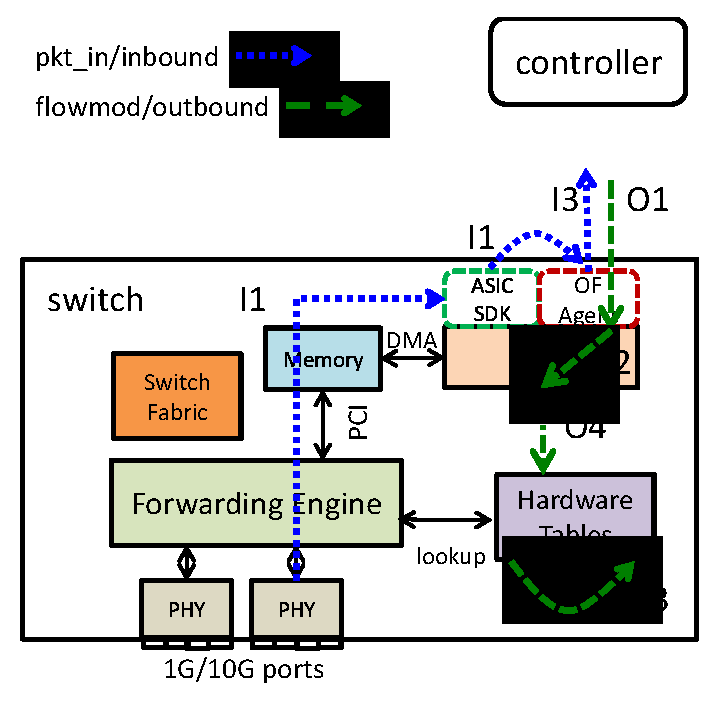
\epsfig{file=./figs/openflow_switch_illustrate.eps,width=0.4\textwidth}
% 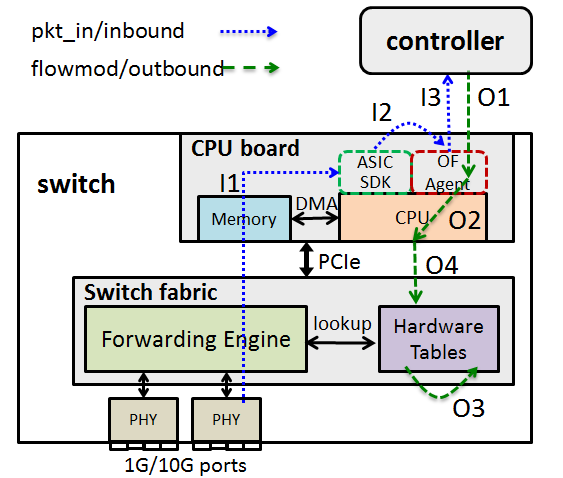
\includegraphics[width=3.5in]{figs/openflow_switch.PNG}
% \caption{Illustration of the t\_in and t\_out delay in an openflow switch.}\label{openflow_switch_delay}
% \end{figure}

% The first contribution of this paper is a systematic exploration of
% latencies in production SDN switches. We study switches from XXX
% \aditya{fill} different vendors under a variety of scenarios that
% carefully isolate the impact of different workload parameters on
% observed latencies. Further, we investigate the relationship between
% switch designs and observed latencies using both active greybox probes
% and feedback from hardware vendors. Key highlights from our
% measurements are as follows: (1) We find that t\_in delays can be as
% high as XXXXms.\aditya{fill} In some cases, poor software support for
% handling \packetin\ message may be an underlying cause, but we note
% that t\_in is always high whenever switch software is also processing
% \packetout\ and \flowmod\ messages. (2) We find that t\_out is
% unusually high as well: for example, inserting a burst of 50 rules
% into a switch based on the Broadcom chipset can take up to 100ms. TCAM
% hardware can support very fast updates, so this delay appears to arise
% primarily from switch software issues. \marina{such as when and what types of rules get puhsed into the TCAM} (3) Priorities can have a
% significant impact: inserting high priority rules into a table
% containing lower priority rules can take as long as XXXs.\aditya{fill}
% This is due to the memory chip's SDK rearranging rules in order of
% priority.

% Crucially, most of the root causes of the latencies are often not
% fundamental and arise due to poor switch software design. Only one
% root cause -- rule rearrangment in face of priorities -- appears to be
% linked to the hardware. A natural question to ask is whether switch
% vendors will improve their software such that most of the latencies we
% observe would go away. We don't believe this is likely: switch vendors
% will not put in the software design effort unless they see the outcome
% as a differentiator. Customers today continue to make purchase
% decisions mostly based on line speeds and perhaps flow table sizes,
% and hence it is likely that we're stuck at least in the near future
% with switch designs that are similar to what we have today.

% \fi

\section{Background}
\label{sec-motivation}

%\fixme{I changed section2 title to Background}
%Our work focuses mainly on switches supporting the popular
%OpenFlow~\cite{openflow} protocol, specifically OpenFlow 1.0, which is
%widely available in production switches today. As we will be clear,
%our results apply qualitatively to more recent versions of OpenFlow
%e.g., OpenFlow 1.3., as well.

%\subsection{Basics}
\iffalse
Instead of running a complex control plane on each switch, SDN delegates
network control to external applications running on a logically central
controller. 
\fi
%In SDN, network control is delegated to external applications running on a
%logically central controller, rather than running a complex control plane on
%each switch. 
\iffalse
Applications determine the routes traffic should take, and they
instruct the controller to update switches with the appropriate forwarding
state. These decisions may be based on data packets that are
received by switches and sent to the controller. Such packet events and
state update operations are enabled by OpenFlow~\cite{openflow}---a standard
API implemented by switches to facilitate communication with the controller.
\fi
%An SDN switch by default does not run control plane protocols, as these are
%delegated to an external application running on a logically central
%controller. Applications determine the routes traffic must take through the
%network and instruct the controller to update the switching substrate with
%the appropriate forwarding state. OpenFlow~\cite{openflow} is a widely
%adopted SDN API employed by switches to communicate with the controller to
%enable such state update operations. 
Although SDN moves control plane logic from switches to a central controller, 
switches must still perform several steps to generate packet events and update
forwarding state. We describe these steps below.
%; we articulate these steps below. 
%\fixme{I cut the sentence after here}
%We then highlight several
%applications whose efficacy is heavily impacted by the latency of these
%control operations on switches. 

% The next section discusses our measurements
% of these latencies, and shows that the root causes of latency are unlikely
% to be eliminated without substantial changes in switch hardware, OpenFlow
% specifications, or control application design.

%\subsection{Components of Latency}

\begin{figure}
\centering
%%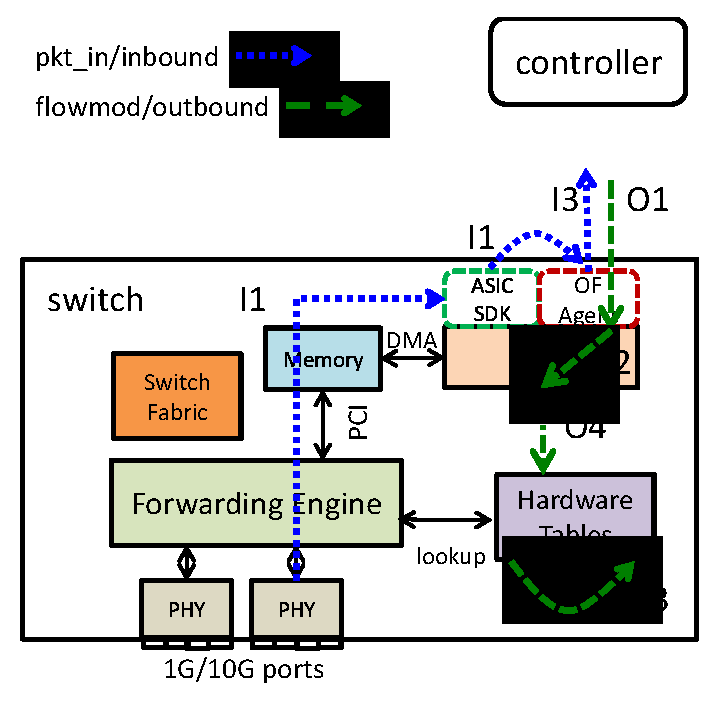
\epsfig{file=./figs/openflow_switch_illustrate.eps,width=0.4\textwidth} %%changed
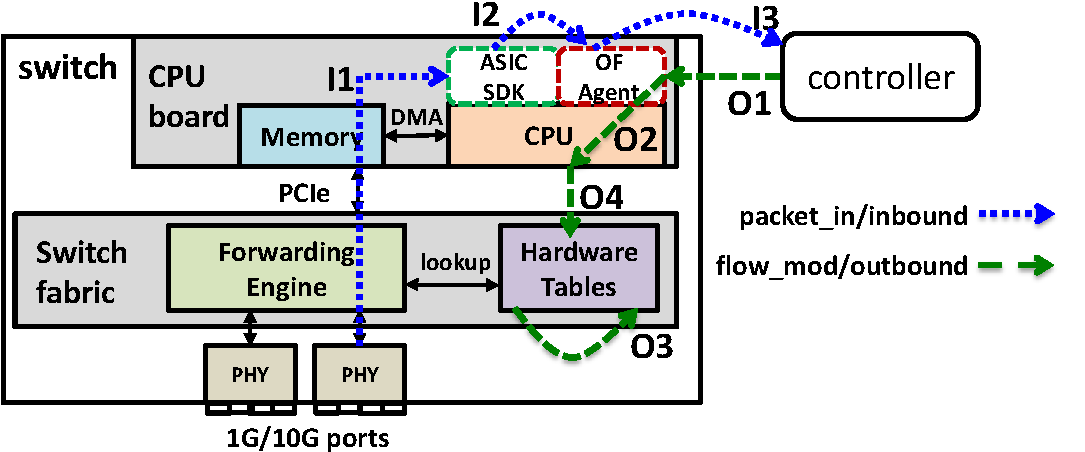
\includegraphics[width=0.98\columnwidth]{figs/openflow_switch.pdf}
\compactcaption{Schematic of an OpenFlow switch. 
%Different rectangular blocks indicate different components of a switch; 
%different boxes do not mean different chips. 
We also show the factors contributing to inbound and outbound latency}\label{openflow_switch_delay}
%\vspace{-0.05in}
\end{figure}

\minisection{Packet Arrival} When a packet arrives, the switch ASIC first
performs a lookup in the switch's hardware forwarding tables. If a match is
found, the packet is forwarded at line rate. Otherwise the following steps
occur (Figure~\ref{openflow_switch_delay}): (I1) The ASIC sends the packet to the switch's CPU via the PCIe bus. (I2) An OS
interrupt is raised, at which point the ASIC SDK gets the packet and
dispatches it to the switch-side OpenFlow agent. (I3) The agent wakes up,
processes the packet, and sends to the controller a \packetin message
containing metadata and the first 128B of the packet. All three steps,
I1--I3, can impact the latency in generating a \packetin message. We
categorize this as {\em inbound latency}, since the controller receives the
message as input.

\minisection{Forwarding Table Updates} 
\iffalse
The application residing on the controller
processes the \packetin, and upon determining a route for packets
belonging to the corresponding flow, sends a \flowmod message and a \packetout
message. \flowmod can also be sent by a controller without receiving a \packetin.

A \flowmod message describes the action the switch should apply to
all future packets of the flow: this could be forward according to some rule,
update an existing rule, or delete a rule. The format of a ``simple''
wildcard rule is \emph{inport=1,dstip=10.0.0.2,action=output:3}.\footnote{In
OpenFlow 1.0, a rule can match up to 12 common header fields.}
The rule may also specify a priority (to determine which rule to apply when
multiple rules match a packet) and a timeout after which the rule is deleted
from the table. 
\fi
The controller sends \flowmod messages to update a
switch's forwarding tables.
A switch takes the following steps to handle a \flowmod
(Figure~\ref{openflow_switch_delay}): (O1) The
OpenFlow agent running on the CPU parses the message. (O2) The agent
schedules the addition (or removal) of the forwarding rule in hardware tables, typically TCAM.  (O3)
Depending on the nature of the rule, the chip SDK may require existing rules
in the tables to be rearranged, e.g., to accommodate high priority rules.
(O4) The rule is inserted (or removed) in the hardware table.  All four steps, O1--O4,
impact the total latency in executing a \flowmod action. We categorize this
as {\em outbound latency}, since the controller outputs a \flowmod message.

\iffalse
A \packetout message releases a specific packet buffered at the switch, and
the switch forwards it as specified in the message. The steps taken by the
switch are the inverse of those for generating \packetin messages; the
latency for these steps is another form of {\em outbound latency}.
\fi

% The actions described above are generally applicable to different
% versions of OpenFlow. \aditya{correct? do we need to say more?}

% In this paper, we focus on the delays imposed at the switch. We ignore
% the impact of the propagation delay to the controller and control
% application processing itself. The latter is typically fast, while the
% former can be made negligible by careful placement of controller
% replicas. \marina{elastic controller placement paper}
\iffalse
\minisection{Application Design} Reactive applications
enforce default-off forwarding to flow sub-spaces; this causes any flow in
that sub-space to generate a \packetin message when it reaches an ingress
switch for the first time. The application then determines the forwarding
action and sends the corresponding \flowmod messages to the switch. These
applications are impacted by both in- and outbound latency.  Proactive
applications directly update forwarding state using \flowmod messages. They
are mainly impacted by outbound latency.
\fi
%\fixme{I deleted subsection Motivating Applications}

\iffalse
\subsection{Motivating Applications}
\label{s:apps}

We now provide examples of both reactive and proactive management
applications that require fine-grained control over data plane state. We
highlight the impact of inbound and outbound latencies on each application's
objectives.

\minisection{Mobility (reactive)} Recent work~\cite{softcell} advocates using
SDN to simplify path setup and management in cellular networks. When
mobile devices want to access the Internet, GPRS Tunneling Protocol (GTP) 
tunnels need to be set up, and reconfigured during handoff.
%In these
%settings, GPRS Tunneling Protocol (GTP) tunnels need to be set up
%whenever an LTE devices want to access the Internet, and reconfigured
%during handoff.
% A control plane entity, called Mobility Management Entity (MME),
% instructs base stations, serving gateways (S-GWs) and packet data
% network gateways (P-GWs) to setup tunnels from base stations to S-GWs,
% and from S-GWs to P-GWs. Recent efforts, e.g.,
% SoftCell~\cite{softcell}, have argued for replacing existing special
% purpose equipment used for S-GW and P-GWs with OpenFlow switches and
% leverage SDN to establish tunnels \aditya{say why, briefly}.
Crucially, these tunnels must be setup within a small latency bound. For 
example, when a mobile device in an idle state wants to communicate with an
Internet server it needs to first transition from idle to connected;
according to recent measurement studies~\cite{MorleyMobisys2012}, the
state transition delay is about 260 ms in LTE. To keep access latency
below 300 ms, as recommended by Web service providers, path setup must
finish in 40 ms. This can be very challenging especially when paths
for multiple devices need to be setup at once, e.g., during a popular
event.
%  \aditya{why? is this trying to say that installing path for a single flow
    %  can easily exceed 40ms? that doesn't seem to be true}. % Similarly,
    %  during handoff, paths % must be reconfigured very fast to avoid
    %  throughput drop.
    
\minisection{Blocking Malicious Web Requests (reactive)} %Blacklisting domain names}
%Another promising reactive application is security. Network administrator can program the network devices and let the packets matching certain fields go to the SDN controller. For example, all DNS traffic can be redirect to the SDN controller and the controller checks whether the flows are trying to access some malicious websites on a blacklist.
%\sourav {Check}
Applications like HP Network Protector~\cite{netprotect} use SDN to
intercept DNS queries from hosts, and drop, forward, or
redirect the request according to global policies. Hosts issuing
many malicious requests can be quarantined by installing high priority rules
that drop traffic from those hosts. As in the mobility scenario, timely
interaction between the controller and switches is critical to avoid 
impacting Web access latencies.

%Applications like HP Network Protector~\cite{netprotect} use SDN to monitor 
%end-host requests and block malicious flows according to globally-defined
%policies. When any device issues a DNS query, the query can be intercepted
%using SDN and the controller can decide to drop, forward, or redirect the
%request. As in the mobility scenario, timely interaction between the
%controller and switch is critical to avoid impacting Web access latencies.

%Applications like BlueCat DNS Director~\cite{} use SDN to provide DNS
%security based on globally administered policies. In these settings, all the
%DNS traffic can be monitored and controlled using the centralized visibility
%and dynamic programmable capabilities that SDN provides. When any device
%attempts connecting to the web, the DNS requests can be intercepted using SDN
%controller to provide a variety of network intelligence like blacklisting
%domain names, redirecting requests, etc. The applicability of SDN in such
%scenario is dependent on timely interaction between the controller and the
%switch so that it does not impact the user perceived latency in accessing web.

\minisection{Failover}
It is possible that SDN can help mitigate the network-wide impact of
failures in wide-area networks, reducing both downtime and congestion
without requiring significant over provisioning. When failures occur,
the SDN management application can quickly compute new paths for flows
traversing failed nodes or links, while also simultaneously rerouting
other high/low priority flows so as to avoid hot-spots~\cite{swan}.
However, this requires significant updates to network state at
multiple network switches. The longer these updates take, the longer
the effect of failure is felt in the form of congestion and drops. We
find that outbound latencies can inflate the time by nearly 20s
(\secref{s:evaluation}) putting into question SDN's applicability to
this scenario. 

\minisection{Intra-Datacenter Traffic Engineering} 
Micro\-TE~\cite{microte}, Hedera~\cite{hedera}, and other recent proposals have
argued for using SDN to route traffic subsets at fine time-scales in order to
achieve fine-grained traffic engineering in data centers. For instance,
MicroTE leverages the fact that a significant fraction of ToR-to-ToR DC
traffic (ToR is ``top-of-rack'' switch) is predictable on short time-scales
of 1-2s. It computes and installs at ToR switches routes for such traffic
on short time-scales. % The computed routes may only be effective for 1-2s
% after which a new sets of routes may be more optimal. 
Thus, latencies in installing routes can significantly undermine MicroTE's
effectiveness. Indeed, we find that updating a set of routes at a ToR switch
in MicroTE can take as long as 0.5s on some SDN switches
(\secref{s:evaluation}). 

\fi
% \times T$s, $n$ is the number of destination ToRs and $T$ is the latency to
% install any give rule. Our measurements presented later in the section
% show the $T \approx 2$ms, so this can be as high as 1s for a
% network with 500 ToR switches. \marina{ref for this number 500 ToR sw} This is significant given that traffic
% predictability may only last for 1-2s. \aditya{more to say here?}

% Hedera makes scheduling and rerouting decisions as often as every few
% seconds for flows exceeding 100MB. However, even such ``elephant''
% flows last a few seconds at most. In some situations, routes for many
% such flows may need to be installed at once at a switch; e.g., when
% many tasks placed in a rack shuffle large intermediate results to
% tasks in other racks, or during data read or data ingest operations in
% big data jobs~\cite{orchestra}. The resulting latency can inflate the
% flows' completion times, and in turn impact job-level performance.


% For path setup from IDLE to CONNECTED, promotion delay is 260ms according to
% Morley's paper. Would this make the path setup not the bottleneck?
% what about voLTE?


% LocalWords:  Intra MicroTE wrt ECMP eval Reactiveness msec Failover handoff
% LocalWords:  SDN GTP LTE GWs GW SoftCell OpenFlow


\section{Latency Measurements}\label{sec-measure}

\begin{figure}
\subfloat[with flow\_mod/pkt\_out \label{fig:intel_inbound_test3}]
  {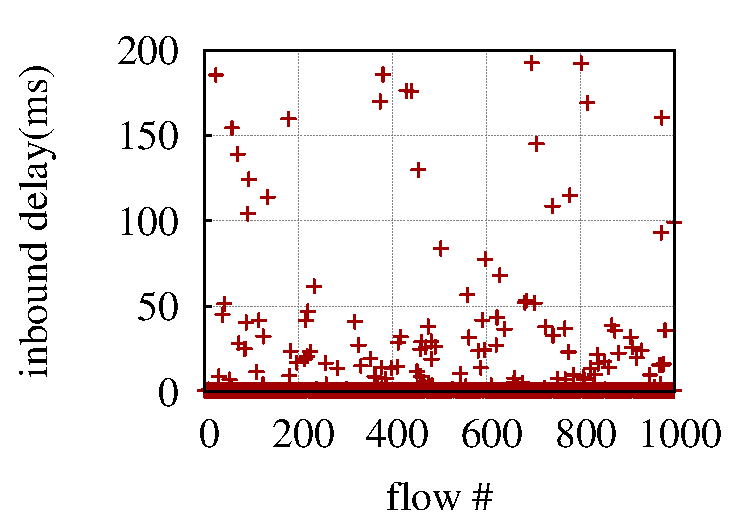
\includegraphics[width=.45\linewidth]{./figs/jan27_intel_inbound_with_pktout_flowmod_rate200.pdf}}
\subfloat[w/o flow\_mod/pkt\_out \label{fig:intel_inbound_test3_wo}]
  {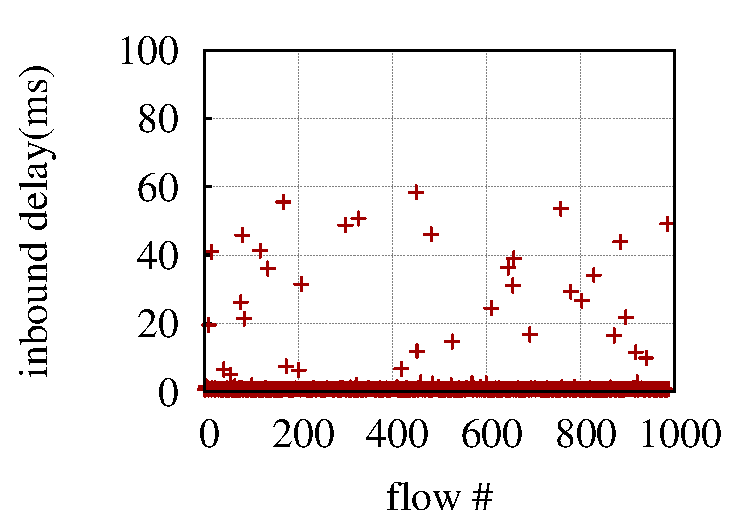
\includegraphics[width=.45\linewidth]{./figs/jan27_intel_inbound_wo_pktout_flowmod.pdf}}
\topcompactcaption{Inbound delay on Intel switch, flow arrival rate = 200/s}
\label{fig:inbound-1}
\end{figure}


\begin{figure*}[!tb]
\centering
\subfloat[burst size 100, same priority\label{fig:bcm_burst_100_same_pri}]
  {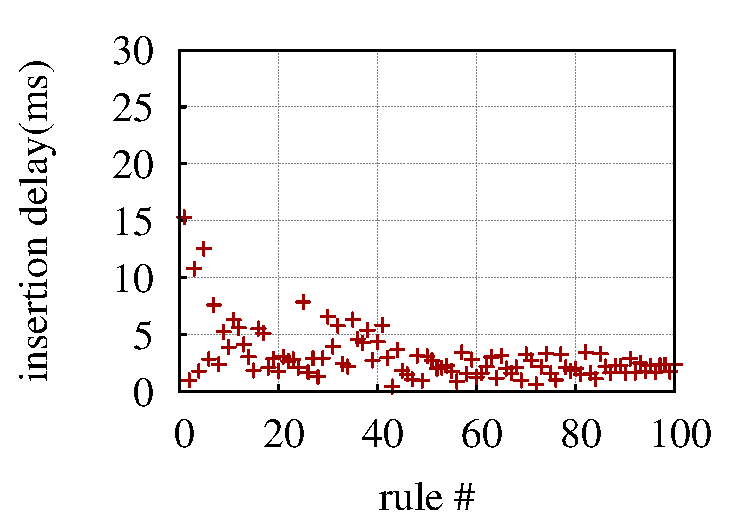
\includegraphics[width=.24\linewidth]{./figs/jan27_bcm_add_same_burst_100.pdf}}\hfill
\subfloat[burst size 200, same priority\label{fig:bcm_burst_200_same_pri}]
  {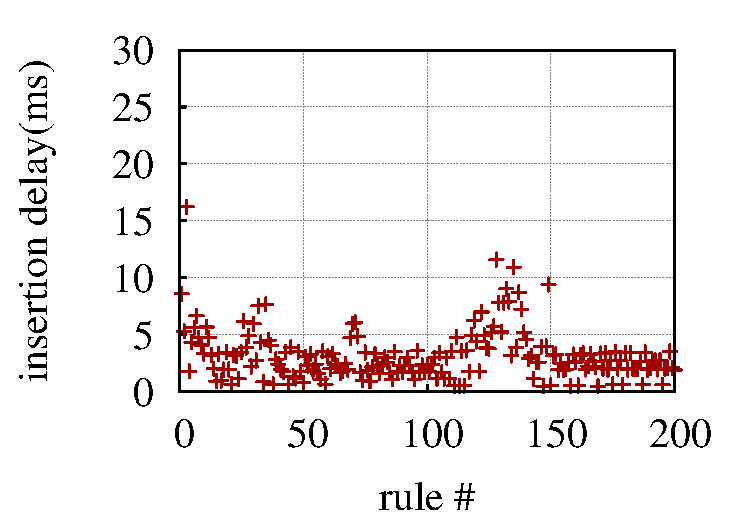
\includegraphics[width=.24\linewidth]{./figs/jan27_bcm_add_same_burst_200.pdf}}\hfill
\subfloat[burst size 100, incr. priority\label{fig:bcm_burst_100_incr_pri}]
  {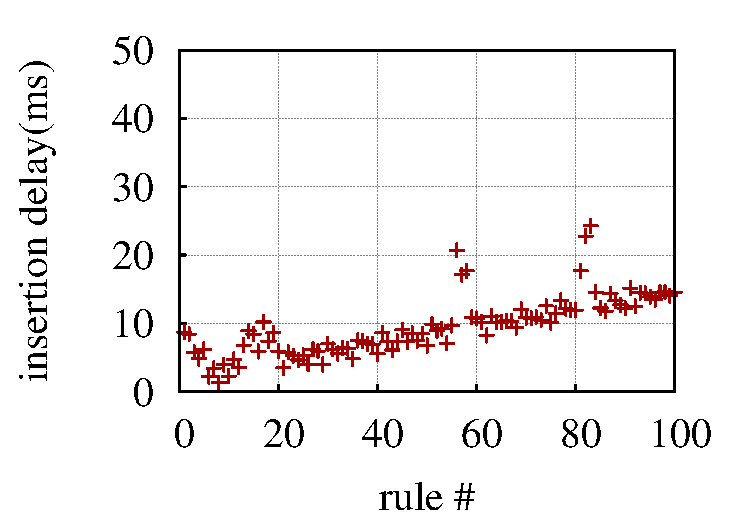
\includegraphics[width=.24\linewidth]{./figs/jan27_bcm_add_incr_burst_100.pdf}}\hfill
\subfloat[burst size 200, incr. priority\label{fig:bcm_burst_200_incr_pri}]
  {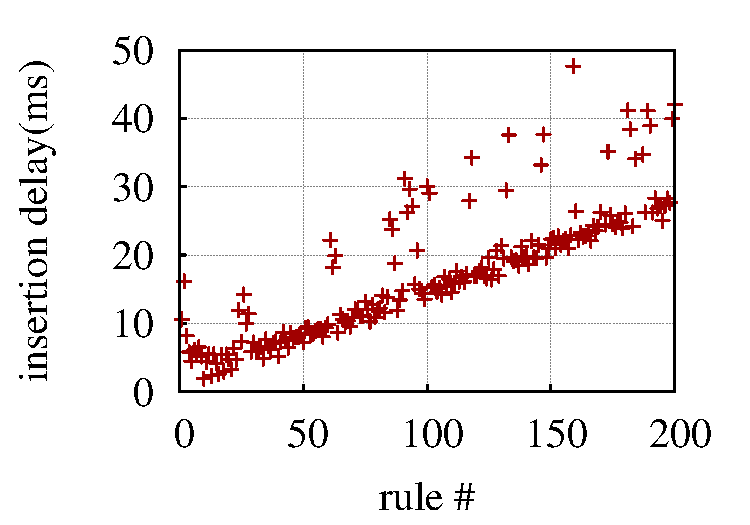
\includegraphics[width=.24\linewidth]{./figs/jan27_bcm_add_incr_burst_200.pdf}}
\topcompactcaption{\BroadcomOne per-rule insertion latency}
\label{fig:priority-broadcom-insert}
\end{figure*}

We conduct measurements on four types of switches from three vendors---Broadcom 956846K with OpenFlow 1.0 firmware (\BroadcomOne) and 
OpenFlow 1.3 firmware (\BroadcomThree), Intel FM6000 (\Intel) and IBM G8264 (\IBM).
We craft our experiments
to ensure the latency impact of various factors can be measured directly from the data plane with the exception of packet\_in generation latency.
\subsection{Dissecting Inbound Latency}
\label{s:measure_inbound}

%%inbound delay on HP
\begin{figure}
% \subfloat[Flow rate = 100/s, concurrent with \flowmod\ and \packetout\ \label{fig:intel_inbound_test1}]
%   {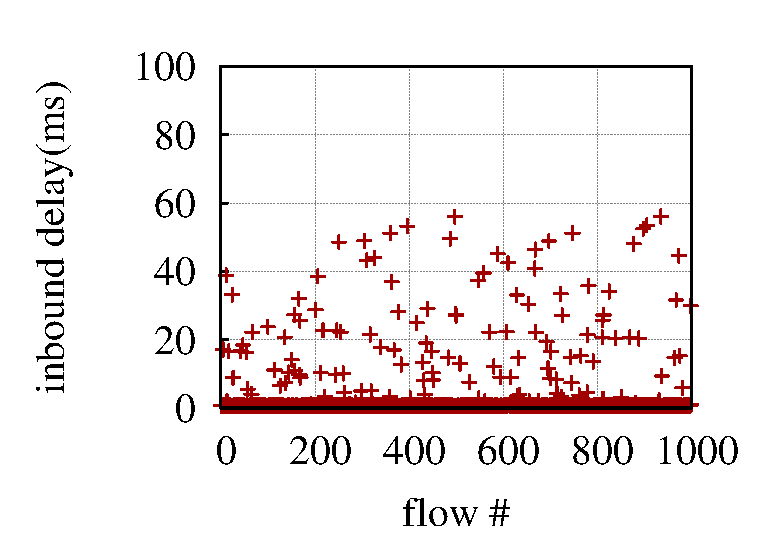
\includegraphics[width=.33\linewidth]{./figs/jan27_intel_inbound_with_pktout_flowmod_rate100.eps}}\hfill
%\subfloat[Flow rate = 200/s\label{fig:hp_inbound_test2}]
%  {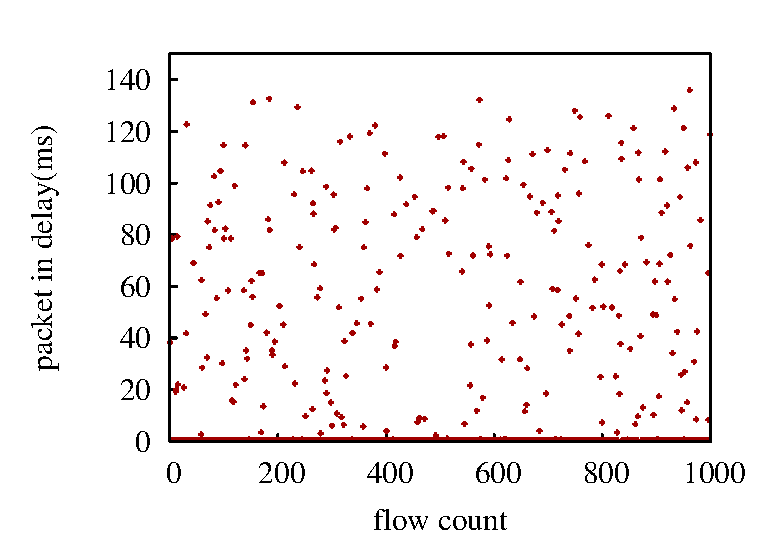
\includegraphics[width=.28\linewidth]{./figs/hp_inbound_delay_200.eps}}\hfill
\subfloat[with flow\_mod/pkt\_out \label{fig:intel_inbound_test3}]
  {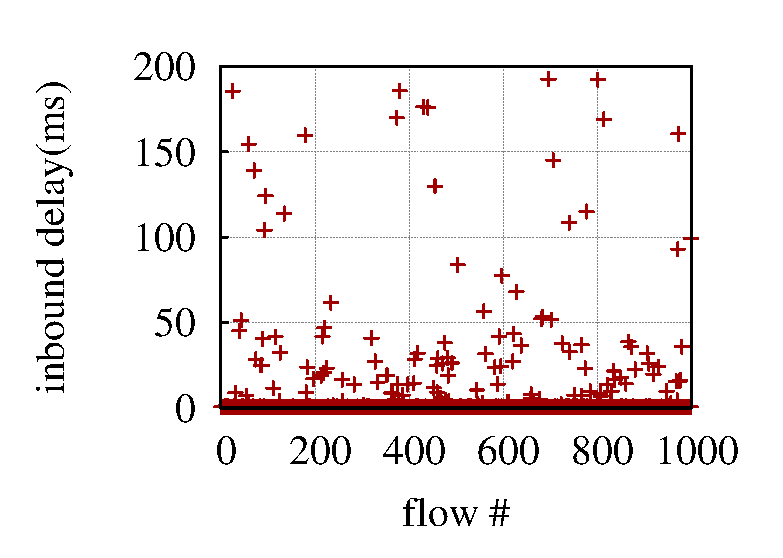
\includegraphics[width=.45\linewidth]{./figs/jan27_intel_inbound_with_pktout_flowmod_rate200.eps}}
\subfloat[w/o flow\_mod/pkt\_out \label{fig:intel_inbound_test3_wo}]
  {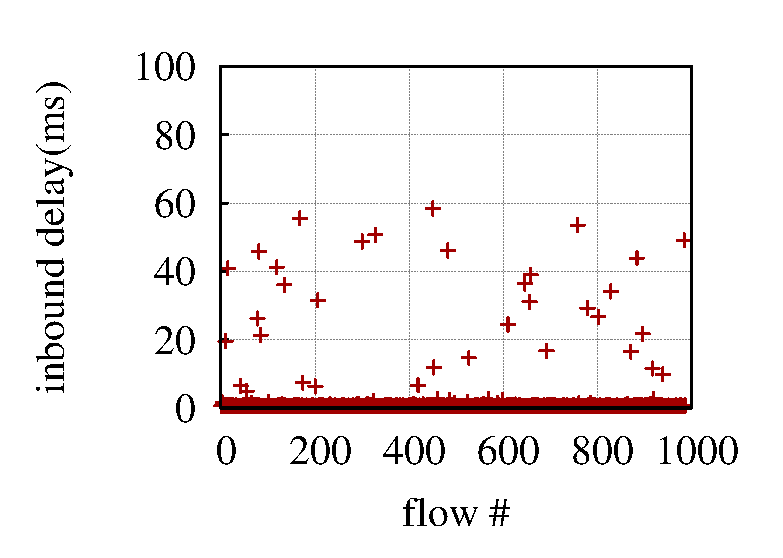
\includegraphics[width=.45\linewidth]{./figs/jan27_intel_inbound_wo_pktout_flowmod.eps}}
\topcompactcaption{{\bf Inbound delay} on {\bf \Intel}, flow arrival rate = 200/s} 
%(a): with concurrent \flowmod\ and \packetout\ operations;
%  (b) without concurrent \flowmod\ and \packetout\ operations}
\label{fig:inbound-1}
\end{figure}

%\emph{Inbound delay:}
To measure inbound latency, we empty the table at the switch, and we generate
traffic such that \packetin events are generated at a certain rate (i.e., we
create packets for new flows at a fixed rate). To isolate the impact of
\packetin processing from other message processing, we perform two kinds of
experiments: (1) the \packetin will trigger corresponding \flowmod (insert
simple OpenFlow rules differing just in destination IP) and \packetout
messages; (2) the\linebreak \packetin message is dropped silently by the
controller. 

We record the timestamp ($t_1$) when each packet is transmitted on the
measurement host's eth1 interface (\figref{experiment_setup}). We also record
the timestamp ($t_2$) when the host receives the corresponding \packetin
message on eth0. The difference ($t_2 - t_1$) is the inbound
latency.\footnote{This measurement technique differs from the approach used
in \cite{ucsdpaper}, where the delay was captured from the switch to the POX
controller which includes the overhead at the controller.}

%\marina{Where are the figures for the inbound delay. Explain how we isolate this
%  type of delay by dropping the pkt at the controller}. 

%%%%HP switch CPU  usage%%%%%%%%%

\begin{table}
\centering
\begin{scriptsize}
\begin{tabular}{cc}
\begin{tabular}{|c|c|c|}
\hline
\multicolumn{3}{|c|}{with flow mod/pkt out} \\ \hline
flow rate & 100/s  & 200/s  \\ \hline
cpu usage & 15.7\%    & 26.5\%   \\ \hline
\end{tabular}
&
\begin{tabular}{|c|c|c|}
\hline
\multicolumn{3}{|c|}{w/o flow mod/pkt out} \\ \hline
flow rate & 100/s   & 200/s \\ \hline
cpu usage & 9.8\%     & 14.4\%   \\ \hline
\end{tabular}
\end{tabular}
\botcompactcaption{CPU usage on \Intel}
\label{fig:inbound-cpu}
\end{scriptsize}
\end{table} 
%\li{is the following sentence correct?}
%When the controller receives \packetin\ message, the controller will drop it. As
%we keep sending packets, it will allow us to repeatedly measure inbound delay. 

Representative results for these two experiments are shown in
\figsref{fig:intel_inbound_test3}{fig:intel_inbound_test3_wo}, respectively,
for the Intel switch; \IBM has similar performance (5ms latency per \packetin on average). 
\BroadcomOne and \BroadcomThree do not support \packetin
messages. For the first experiment, we see that the inbound latency is quite
variable with a mean of 8.33ms, a median of 0.73ms, and a standard deviation
of 31.34ms. For the second experiment, the inbound delay is lower (mean of 
1.72ms, median of 0.67ms) and less variable (standard deviation of 6.09ms). 
We also observe that inbound latency depends on the \packetin rate: e.g. in
first experiment the mean is 3.32 ms for 100 flows/s (not shown) vs. 8.33ms
for 200 flows/s (\figref{fig:intel_inbound_test3}).

The only difference between the two experiments is that in the former case
the switch CPU must process \flowmod and \packetout messages, and send
forwarding entries and outbound packets across the PCIe bus to the ASIC, in
addition to generating \packetin messages. As such, we observe that the CPU
usage is higher when the switch is handling concurrent OpenFlow operations and
generating more \packetin messages (\tabref{fig:inbound-cpu}). However, since
the Intel switch features a powerful CPU (\tabref{switch_para}), plenty of
CPU capacity remains. Our conversations with the switch vendor suggest that
the limited bus bandwidth between the ASIC and switch CPU is the primary
factor contributing to inbound latency. 

%Thus, we conclude
%that the switch CPU is one of the potential causes for the inbound
%latency.\aaron{Do we still think this is true? If the CPU is only 26.5\%
%    utilized, why does latency increase?} Further, our conversations with the
%    switch vendor suggest that the limited bus bandwidth between the ASIC and
%    switch CPU also contributes to the inbound latency. 
%%But they also note that the ASIC-CPU bandwidth is just around 10Mbps.  Thus,
%    %we conclude that inbound delay is mainly caused by switch CPU and due to
%    %interference with \flowmod\ and \packetout\ processing. 
%\sourav {The above lines may have to be re-written. Please check}
 

\subsection{Outbound Latency} 
\label{s:outbound_meas}

We study the outbound latencies for three different \flowmod\
operations: insertion, modification, and deletion. For each operation, we
examine the latency impact of key factors, including flow table
occupancy and rule priority.


\subsubsection{Insertion Latency}
\label{s:meas_insert}

\begin{figure*}[!tb]
\centering
\subfloat[burst size 100, same priority\label{fig:bcm_burst_100_same_pri}]
  {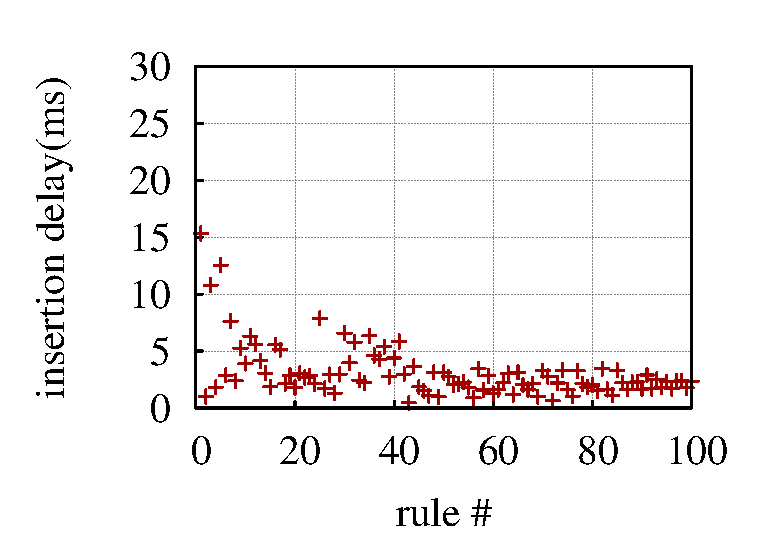
\includegraphics[width=.24\linewidth]{./figs/jan27_bcm_add_same_burst_100.eps}}\hfill
\subfloat[burst size 200, same priority\label{fig:bcm_burst_200_same_pri}]
  {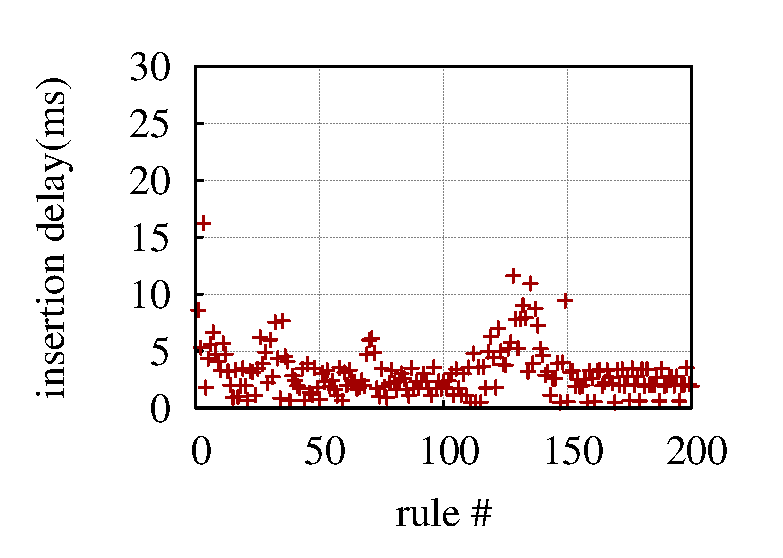
\includegraphics[width=.24\linewidth]{./figs/jan27_bcm_add_same_burst_200.eps}}\hfill
\subfloat[burst size 100, incr. priority\label{fig:bcm_burst_100_incr_pri}]
  {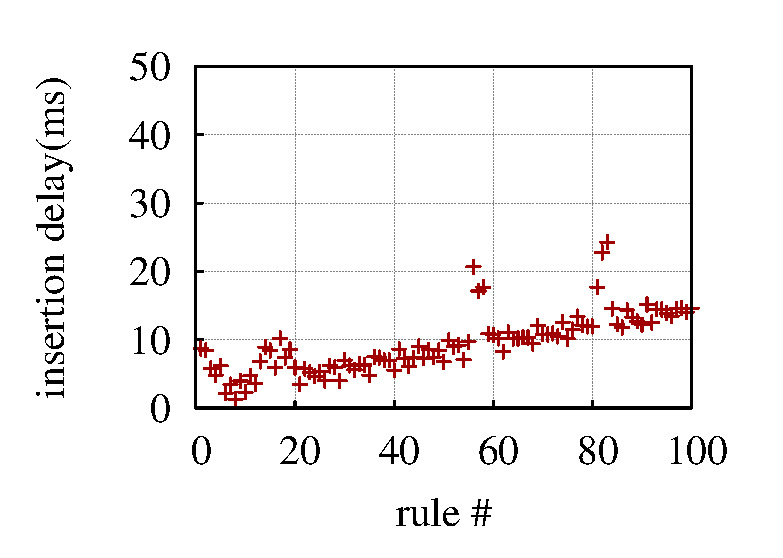
\includegraphics[width=.24\linewidth]{./figs/jan27_bcm_add_incr_burst_100.eps}}\hfill
\subfloat[burst size 200, incr. priority\label{fig:bcm_burst_200_incr_pri}]
  {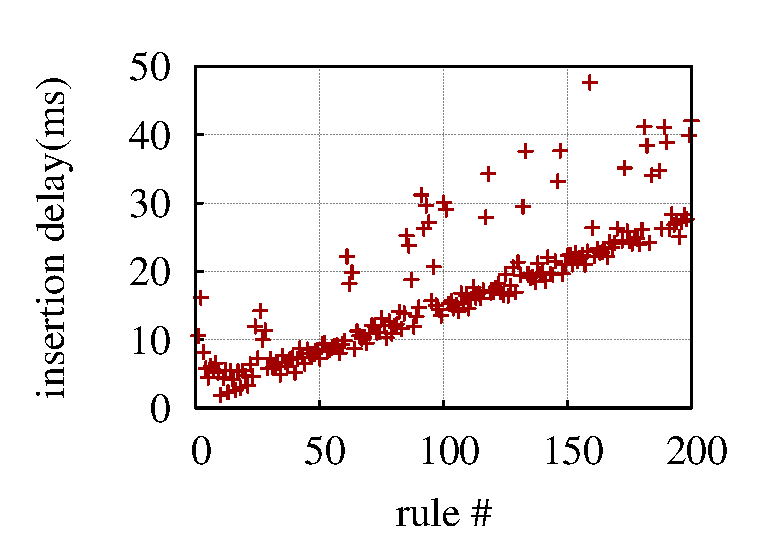
\includegraphics[width=.24\linewidth]{./figs/jan27_bcm_add_incr_burst_200.eps}}
\topcompactcaption{{\bf \BroadcomOne} priority per-rule {\bf insert} latency}
\label{fig:priority-broadcom-insert}
\end{figure*}


We first examine how different rule workloads impact insertion latency. We
insert a burst of $B$ rules: $r_1,\cdots,r_B$. Let $T(r_i)$ be the time we
observe the first packet matching $r_i$ emerging from the output port
specified in the rule. We define per-rule insertion latency as $T(r_i)-T(r_{i-1})$.  

%We conduct a variety of tests to examine how different patterns of
%rule workloads impact insertion latency. In almost all experiments, we
%install a burst of rules. Let us denote these rules
%in a sequence as $r_1, r_2,\cdots,r_i,\cdots, r_B$. Denote $T(r_i)$ as the time we
%observe the first packet matching $r_i$ emerging from the intended port of the rule
%action. We define insertion latency as $T(r_i)-T(r_i-1)$.  

\minisection{Rule Complexity} 
To understand the impact of rule complexity (i.e., the number of header 
fields specified in a rule), we install bursts of rules that specify either
2, 8, or 12 fields. In particular, we specify destination IP and EtherType
(others wilcarded) in the 2-field case; input port, EtherType, source and
destination IPs, ToS, protocol, and source and destination ports in the
8-field case; and all supported header fields in the 12-field (exact match)
case. We use a burst size of 100 and all rules have the same priority.

%To understand the impact of rule complexity (i.e., the number and type of
%matching fields specified in a rule), we conduct three different
%experiments with a fixed burst size ($B$ = 100) and priority but the rules
%having different matching fields. In the first experiment, all the rules in a
%burst only have only 2 match fields (others wildcarded), in the second
%experiment all the rules have 8 match fields (others wildcarded), and in the
%third experiment the rules have all the 12 match fields set (exact match).
%For the 2-match field experiment, we specified the destination IP and
%EtherType as the matching fields and for the 8-match field experiment we
%specified all the matching fields except source mac, destination mac, vlan id
%and vlan priority.  

We find that rule complexity {\em does not} impact insertion latency. The
mean per-rule insertion delay for 2-field, 8-field, and exact
match cases is 3.31ms, 3.44ms, and 3.26ms, respectively, for \BroadcomOne.
Similarly, the mean per-rule insertion delay for \Intel, \IBM, and
\BroadcomThree is $\approx$ 1 ms irrespective of the number of fields. 
All experiments that follow use rules with 2 fields.

%\emph{\BroadcomOne:} The mean per rule insertion delay is 3.31, 3.44 and 3.26 ms for 2-match field, 8-match field and exact match experiments respectively. This indicates that the insertion time does not vary with rule complexity on \BroadcomOne.

%\emph{\BroadcomThree:} 
%We observed that when a burst of rules is inserted, the \BroadcomThree firmware organizes the rules into batches. 
%Each batch has a size of about 50 rules and a single batch of rules is scheduled for insertion every 4 seconds. 
%This effect adds significant delay (4 seconds) between processing of two consecutive batches.
%This can be attributed to the inefficent firmware implementation which is still in its early stage of development. 
%We assume that the batching effect is due to unoptimized firmware and will be fixed in the near future. 
%Hence, we only consider the batch completion time when discussing insertion time on \BroadcomThree.  


%For 2-field, 8-field and exact match experiments the mean batch completion time 
 %(mean per rule insertion time) 
%is about 47 ms, 45 ms, 51 ms. This indicates that the %insertion time is not dependent on rule complexity on %\BroadcomThree neither. 

\minisection{Table occupancy} To understand the impact of table occupancy, we
insert a burst of $B$ rules into a switch that already has $S$ rules
installed. All $B+S$ rules have the same priority. We fix $B$ and
vary $S$, ensuring $B+S$ rules can be accommodated in each switch's hardware
table.

%\li{TODO: Keqiang, please add corresponding numbers in text for Broadcom and
%  Intel. } 

We find that flow table occupancy {\em
does not} impact insertion delay if all rules have the same priority.
Taking $B=400$ as an example, the mean per-rule insertion delay is 3.14ms, 
1.09ms, 1.12ms, and 1.11ms (standard deviation 2.14ms, 1.24ms, 1.53ms, and
        0.18ms) for \BroadcomOne, \BroadcomThree, \IBM
and \Intel, respectively, regardless of the value of $S$. 
%However, flow table occupany has an indirect impact through priority which
%we will cover next.  investigate in Section~\ref{sec:priority}. 

\minisection{Rule priority} To understand the effect of rule priority on the
insertion operations, we conducted three different experiments each covering
different patterns of priorities. In each, we insert a burst of $B$ rules
into an empty table ($S=0$); we vary $B$. In the {\em same priority}
experiment, all rules have the same priority. In the {\em increasing} and
{\em decreasing priority} experiments, each rule has a different priority and
the rules are inserted in increasing/decreasing priority order, respectively. 

\emph{\BroadcomOne, same priority.} 
%We experimented with several values of $B$. 
Representative results for $B=100$ and $B=200$ are shown in
\figsref{fig:bcm_burst_100_same_pri}{fig:bcm_burst_200_same_pri}, respectively. In both
cases, we see that the per-rule insertion delay is similar: with
medians of 3.12ms and 3.02ms, and standard deviations of 1.70ms and 2.60ms, 
for $B=100$ and $B=200$, respectively. 
% insert $B=100$ rules in the
% switch. As shown in Figure~\ref{fig:priority-broadcom-insert}-a, the per rule
% insertion delay among the 100 rules are similar with median xx ms and standard
% deviation xx. As shown in Figure~\ref{fig:priority-broadcom-insert}-b, the
% insertion delay for burst size 200 has a median xx ms and standard deviation
% xx. We also perform other burst sizes. The results are similar.
We conclude that same priority rule insertion delay does not vary with burst size on \BroadcomOne.

\emph{\BroadcomOne, increasing priority.}
\figref{fig:bcm_burst_100_incr_pri} shows the result for
$B=100$. We note that the per-rule insertion delay actually {\em
  increases linearly} with the number of
rules inserted. \figref{fig:bcm_burst_200_incr_pri}
shows the result for $B=200$; we see that the slope stays the same as
$B=100$.
%\aaron{This is hard to see visually because
%    \figref{fig:bcm_burst_100_incr_pri} and
%        \figref{fig:bcm_burst_200_incr_pri} have different maximum x values} 
Compared with the same priority experiment, the average per-rule
delay is much larger: 9.47ms (17.66ms) vs 3.12ms (3.02ms), for $B=100$ (200). 
Results for other values of $B$ are qualitatively similar. 
%li: does not parse, rewrite
%Thus, the latency experienced
%by a rule can be impacted by when the priorities of rules inserted
%immediately ahead of it are lower.
The TCAM in this switch stores high priority rules at low (preferred)
memory addresses. Thus, each rule inserted in this experiment
displaces all prior rules!

\emph{\BroadcomOne, decreasing priority.} 
We also perform decreasing priority insertion (not shown). The average 
per-rule insertion delays for $B=100$ and $B=200$ are 8.19ms and 15.5ms, respectively. We observe that the burst of $B$ rules is divided into a number 
of groups, and each group is reordered and inserted in the TCAM in order of increasing priority. 
%\aditya{the following is weird} We have been
%working with Broadcom in our measurements. The feedback is that Broadcom has not
%optimized their software to handle rule priority optimally in all cases.
This indicates that \BroadcomOne firmware reorders the rules and prefers
increasing priority insertion. 
%\keqhe{The average per-rule insertion delays for $B=100, B=200$ with decreasing priority are 8.19ms and 15.5ms respectively.}\aaron{We need some numbers here so we can
%compare against them in the \BroadcomThree results below.}

\iffalse
\emph{\BroadcomThree.} 
In \BroadcomThree we observed that when a burst of rules is inserted, 
the firmware organizes the rules into batches. 
Each batch has a size of about 50 rules and a single batch of rules is scheduled for insertion every 4 seconds. 
This effect adds significant delay (4 seconds) between processing of two consecutive batches. 
This can be attributed to the inefficent firmware implementation which is still in its early stage of development. 
We assume that the batching effect is due to unoptimized firmware and will be fixed in the near future. Hence, 
we ignore the inter-batch processing delays and only consider the batch completion time.  
\sourav {I am not sure if this a correct way of addresing this. 
What should we say here? The reasons for this batching effect are still unknown}
\fi
\emph{\BroadcomThree, same priority.} 
The mean per-rule insertion
delay is 1.09ms (1.08ms) for $B=100$ (200). Thus, similar to \BroadcomOne,
the rule insertion time does not vary with burst size when all rules are of
the same priority. 

\emph{\BroadcomThree, increasing priority.} 
The average per-rule insertion delay is much 
larger: 7.75ms (16.81ms) for $B = 100$ (200). This is similar to our findings
for \BroadcomOne, affirming that TCAM organization requirements, not software
implementation issues, are the primary cause.
%This shows that the TCAM organization in case of \BroadcomThree is similar to that of \BroadcomOne where high priority rules are stored at low memory addresses. 


%the mean completion time (per rule insertion time)  for 1st, 2nd, 3rd and 4th batch is 284 (5.68), 589 (11.78), 1192 (23.84) and 2022 (40.44) ms respectively which is significantly higher than the same priority completion time. This shows that the TCAM organization in case of \BroadcomThree is similar to that of \BroadcomOne where high priority rules are stored at low memory addresses. 

\emph{\BroadcomThree, decreasing priority.} 
The per-rule delay is similar to that of
same priority insertion: $\approx 1$ms. This contrasts with
\BroadcomOne, where decreasing priority insertion increases with the
number of rules inserted---average of 8.19ms (15.5ms) for $B=100$ (200). 
Hence the \BroadcomThree firmware has been better optimized to handle 
decreasing priority rule insertions.

%\fixme{below is added}

\emph{\IBM, same priority.}
The \IBM switch's same priority rule insertion performance
trend is quite similar to that of \Broadcom. When all the inserted rules
have the same priority, the per-rule insertion latency is around 1.1ms.

\emph{\IBM,  increasing priority.}
When it comes to increasing priority, the per-rule insertion latency becomes significantly larger.
The average per-rule insertion delays for $B=100$ and $B=200$ are 10.14ms and 18.63ms, respectively. 

\emph{\IBM,  decreasing priority.}
\IBM switch's per-rule insertion latency in decreasing priority is similar to that of same priority
rule insertion, namely, around 1.1ms per insertion.
%This shows that \BroadcomThree optimizes decreasing priority rule insertions 
%efficiently unlike \BroadcomOne. \aaron{Fix the preceding sentence after we
%have numbers in \BroadcomOne decreasing priority above.}
%In case of increasing priority experiment the per rule insertion delay increases with increase in burst size. Compared with the same priority experiment the average per rule insertion delay in this case is larger: ??? (???) vs ??? (???) for B = 100 (200). However for decreasing priority experiment,  the delay is much smaller than  \BroadcomOne and does not vary with the burst size. The mean delay for   
%for B = 100 and 200 is ??? and ??? ms respectively. This shows that while the 
%\BroadcomThree firmware is more optimized than \BroadcomOne firmware  for decreasing priority rule insertion, the delays are still large for increasing priority rule insertion because of the way TCAM organizes rules in the table(high priority at low memory addresses).

% We next show our measurement results on Intel. 

\begin{figure}[!tb]
\centering
%\subfloat[burst size 800, same priority.\label{fig:intel_burst_800_same_pri}]
 %{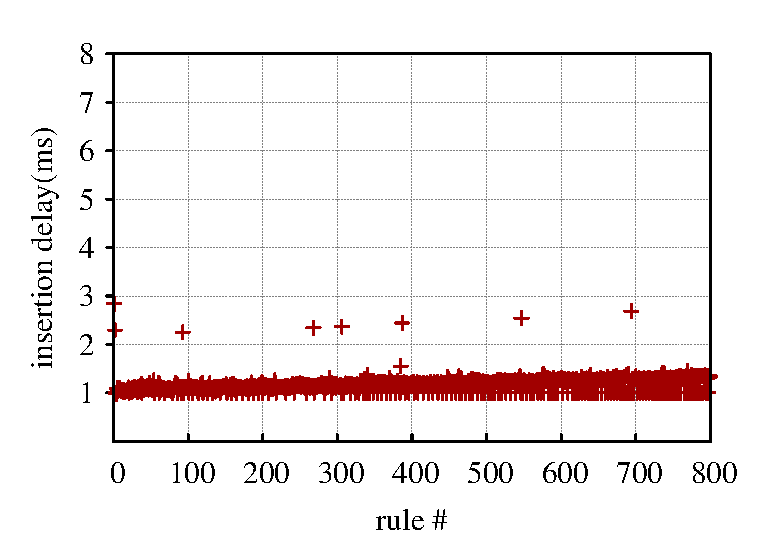
\includegraphics[width=.33\linewidth]{./figs/jan27_intel_same_burst_800.eps}}\hfill
%\subfloat[burst size 200, same priority.\label{fig:intel_burst_200_same_pri}]
%  {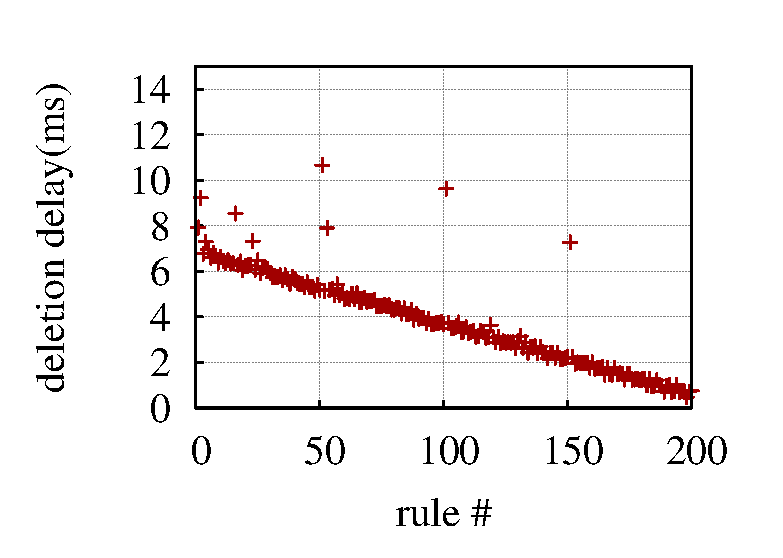
\includegraphics[width=.24\linewidth]{./figs/jan27_intel_same_burst_200.eps}}\hfill
\subfloat[burst size 800, incr. priority\label{fig:intel_burst_800_incr_pri}]
  {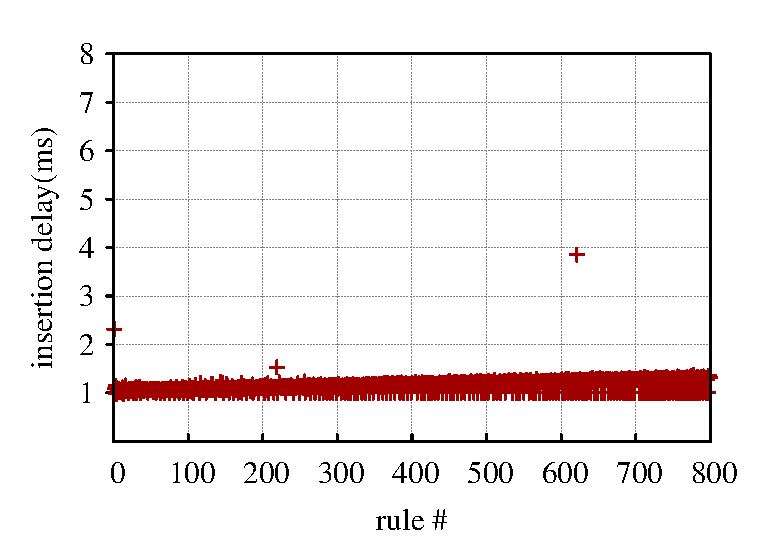
\includegraphics[width=.49\linewidth]{./figs/jan27_intel_incr_burst_800.eps}}\hfill
\subfloat[burst size 800, decr. priority\label{fig:intel_burst_800_decr_pri}]
 {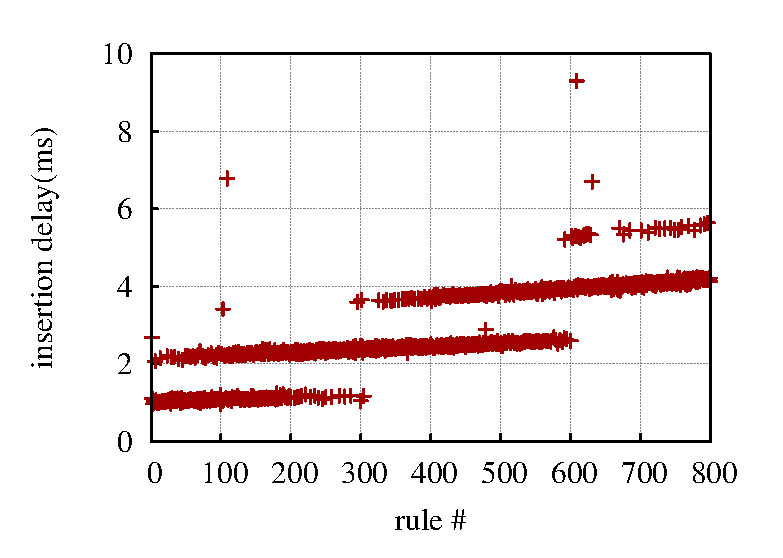
\includegraphics[width=.49\linewidth]{figs/jan27_intel_empty_800L_decr_delta.eps}}
%\subfloat[burst size 200, decreasing priority.\label{fig:intel_burst_200_incr_pri}]
%  {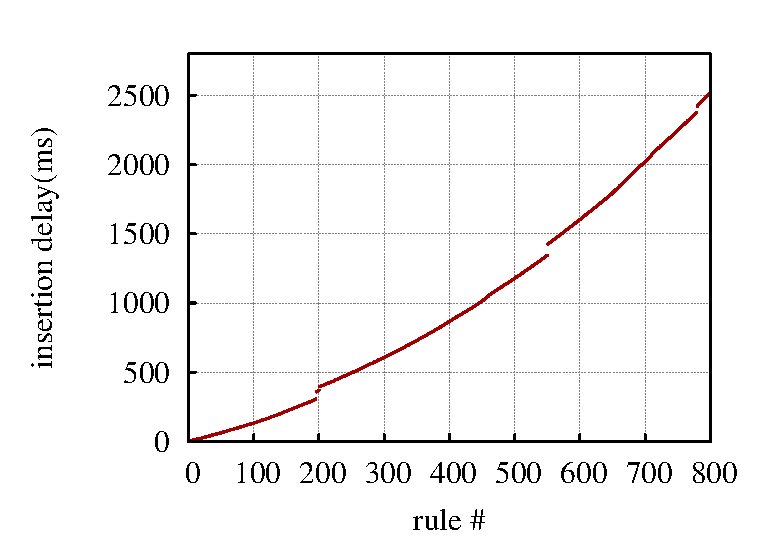
\includegraphics[width=.24\linewidth]{figs/jan27_intel_3200H_800L_decr_real.eps}
\topcompactcaption{{\bf Intel} priority per-rule {\bf insert}
%: (a) burst size
%  100, same priority (b) burst size 200, same priority (c) burst size 100,
%  increasing priority (d) burst size 200, increasing priority {\bf TODO: (e) burst size
%  100, decreasing priority (f) burst size 200, decreasing priority; SHOW the
%  priority effect}
} 
\label{fig:priority-intel-insert}
\end{figure}

\emph{\Intel, same priority.} %Figure~\ref{fig:priority-intel-insert}(a)
For $B=800$ on \Intel\footnote{We present results for a larger value of $B$ 
because the flow table size on \Intel is larger (\tabref{switch_para}).} we see that the per-rule
insertion delay is similar across the 800 rules, with a median of 1.17ms and
standard deviation of 0.16ms (not shown). 
% \aaron{It is odd to show results for B=100 and B=200 for \BroadcomOne, but B=800 for Intel? Do we have higher values of B (e.g., B=600) for \BroadcomOne, so we can use the same B value(e.g., B=600) for both?} 
The results for other values of $B$ are similar. Thus, similar to
\BroadcomOne, \BroadcomThree, and \IBM same priority rule insertion delay does 
not vary with burst size on \Intel. 
%The result for $B=200$ in
%Figure~\ref{fig:priority-intel-insert}(b) shows a similar trend with a
%median delay of xx ms and a standard deviation of
%xx. \aditya{the two sets of lines is interesting and merits
%  discussion!} Thus, similar to Broadcom, same priority rule insertion
%delay does not vary with burst size on Intel.
% we see that the
% same-priority rules isinsertion of a higher priority rule is totally unimpacted by the lower
% priority rules inserted immediately ahead of it. 
% priority rule insertion delay does not vary with burst size on Intel,
% similar to Broadcom.

\emph{\Intel, increasing priority.} %\aditya{graphs for this are missing}
\figref{fig:intel_burst_800_incr_pri} shows per-rule latencies for
$B=800$. \emph{Surprisingly}, in contrast with \BroadcomOne,
\BroadcomThree, and \IBM, the per rule
insertion delay among the rules is more or less the same, with a
median of 1.18ms and a standard deviation of 1.08ms.  We see similar
results for other values of $B$. This shows that the \Intel TCAM architecture 
is fundamentally different from \Broadcom. 
%\aditya{is this a hardware  difference? can it not be SDK?} 
%li: yes, hardware 
Rules are ordered in \Intel's TCAM such that higher priority rule insertion
does not displace existing low priority rules. 
%\aditya{why are we talking about displacement here? we did not mention this for
%broadcom} 

\emph{\Intel, decreasing priority.} %\aditya{graphs for this are missing} 
%The insertion delay increases for decreasing priority insertion.  Rule arrangement in
%  TCAM is such that low priority rule insertion causes displacement of high
%  priority rules. \aditya{this does not appear to be true}
\figref{fig:intel_burst_800_decr_pri} shows per-rule insertion latencies for
$B=800$. We see two effects: (1) the latencies alternate between two modes at any
given time, and (2) a step-function effect after every 300 or so
rules. 


A likely explanation for the former is bus buffering. Since rule insertion is 
part  of the switch's control path, it is not really optimized for latency.
The latter effect can be explained as follows: Examining the \Intel switch architecture, we
find that it has 24 slices, $A_1\ldots A_{24}$, and each slice holds 300
flow entries. There exists a consumption order (low-priority first) across
all slices.  Slice $A_i$ stores the $i^{th}$ lowest priority rule group. If
rules are inserted in decreasing priority, $A_1$ is consumed first until it
becomes full. When the next low priority rule is inserted, this causes one
rule to be displaced from $A_1$ to $A_2$.  This happens for each of the next
300 rules, after which cascaded displacements happen: $A_1 \rightarrow A_2
\rightarrow A_3$, and so on. We confirmed this with \Intel.
%\aditya{we dont have a good explanation for 1}

% ; then $A_2$ starts to be consumed. However, due to the
% decreasing order, 299 existing rules in $A_1$ must be moved into $A_2$, and
% then a new inserted rule will be written into slice $A_1$ until it
% becomes full.
%full, and so on. 


%We suspect some rules trigger
%TCAM reordering and some do not. This results in an ON and OFF process that adds
%delay if the process is on.  
%\aditya{the following is weird} We have been working with Intel closely on our
%measurements. The feedback we got 
%from Intel is that their switch firmware has not been optimized to handle rule
%priorities efficiently in all cases.
%\li{are the two modes strictly alternative? Even rule number mode 1, odd rule
%  number mode 2??}

\minisection{Priority and table occupancy combined effects} 
%Given our understanding of the impact of rule priority and table occupancy on
%per-rule insertion latency, we now study their combined impact. 
We now study the combined impact of rule priority and table occupancy.
We conduct two experiments: For the first experiment, the table starts with
$S$ high priority rules, and we insert $B$ low priority rules.  For the
second experiment, the priorities are inverted.
For both experiments, we measure the total time to install all rules in the
burst, $T(r_B)-T(r_1)$.
%burst rule insertion completion time;
%many applications depend on this the metric (\secref{s:apps}). 

\begin{figure}
\subfloat[insert low priority rules into\newline a table with high priority rules\label{fig:bcm_outbound_two_pri_high_low_burstB}]
  {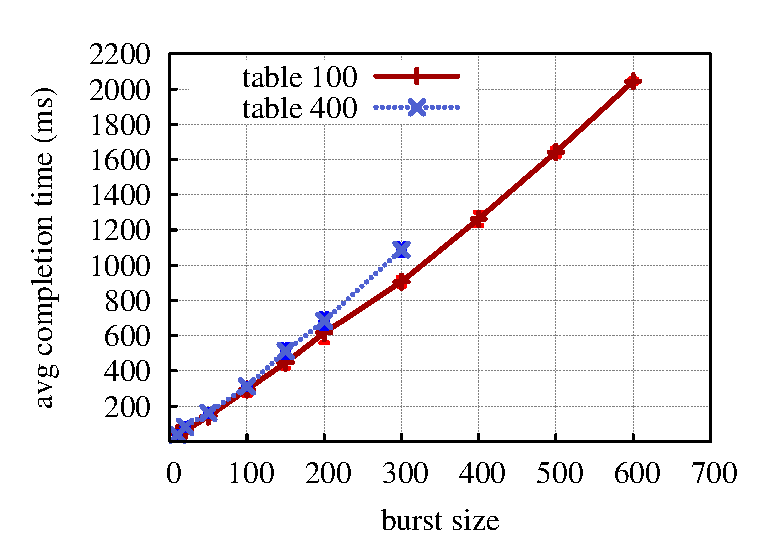
\includegraphics[width=.50\linewidth]{./figs/bcm_two_pri_high_low_burstB.eps}}\hfill
\subfloat[insert high priority rules into a table with low priority rules\label{fig:bcm_outbound_two_pri_low_high_burstB}]
  {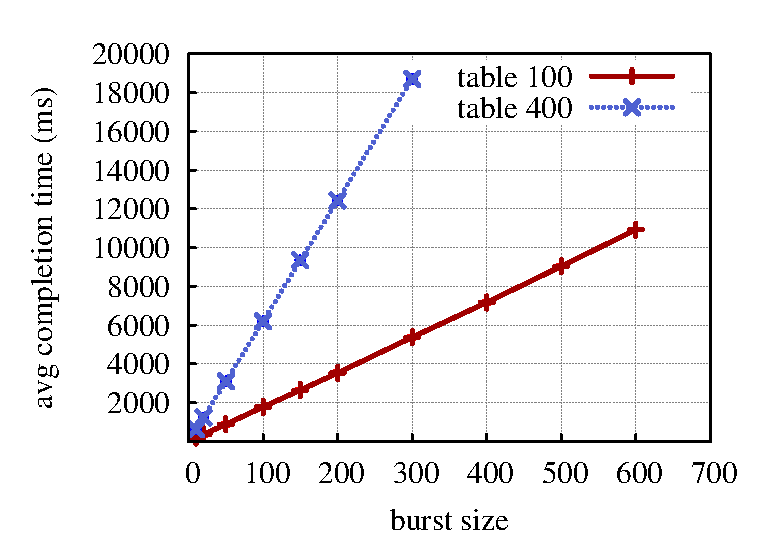
\includegraphics[width=.50\linewidth]{./figs/bcm_two_pri_low_high_burstB.eps}}
\compactcaption{Overall completion time on {\bf \BroadcomOne}.  Initial table occupancy is S high (low) priority rules; insert a burst of low (high) priority rules. Averaged over 5 runs. }
\label{fig:burst-completion-time}
\end{figure}

%We conduct two experiments. With $S$ rules in the table, we insert a burst of $B$ rules. 
%For the first experiment, $S$ has high priority and we insert the burst with low priority. 
%For the second experiment, if it is Broadcom (\BroadcomOne or \BroadcomThree), $S$ has low priority and we insert rules with high priority; if it is Intel, $S$ has high priority and we insert rules in {\em decreasing} priority.

For \BroadcomOne, \BroadcomThree, and \IBM, we expect that as long as the same
number of rules are displaced, the completion time for different values of
$S$ should be the same.
Indeed, from \figref{fig:bcm_outbound_two_pri_high_low_burstB} (for
\BroadcomOne), we see that even with 400 high priority rules in the
table, the insertion delay for the first experiment is no different from the
setting with only 100 high priority rules in the table. In contrast, in
\figref{fig:bcm_outbound_two_pri_low_high_burstB}, newly inserted high
priority rules will displace low priority rules in the table, so when
$S=400$ the completion time is about 3x higher than $S=100$.
%\fixme{added IBM below}
For \IBM (not shown), inserting 300 high priority rules into a table with 400
low priority rules takes more than 20 seconds.  

 
\iffalse
\begin{figure}[!tb]
\centering
\subfloat[decreasing priority\label{fig:intel_burst_100_incr_pri_1}]
  {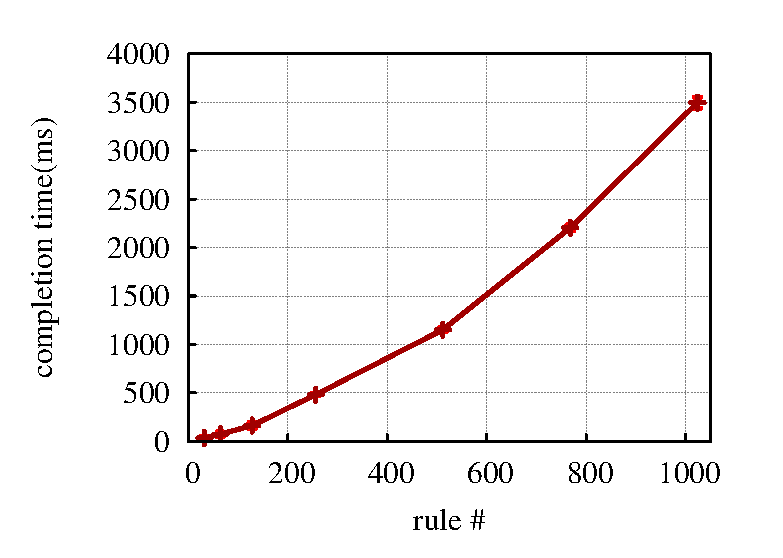
\includegraphics[width=.5\linewidth]{./figs/jan27_intel_decr_burst_size_effect.eps}}\hfill\caption{{\bf Intel} overall completion time} 
\label{fig:priority-intel-insert-more-results}
\end{figure}
\fi

%For \Intel, we also run the same two experiments as for Broadcom. 
For \Intel, the results are similar to same priority rule insertion. This
indicates that \Intel uses different TCAM organization schemes than the
\Broadcom and \IBM switches.  %\fixme{changed}
%optimizes for rule priority better than \BroadcomOne. 
\iffalse
When
we insert in decreasing priority
(\figref{fig:priority-intel-insert-more-results}) the completion time is
about 3.5 seconds, 3x higher than the case of same priority insertion.
\aaron{What is the point of these Intel results?}
\sourav{To show the worst case burst completion time on Intel since it does not have table occupancy effect. But now since the title has been changed from burst completion time to combined effect, I dont think this makes much sense here. }
 \fi
 
\minisection{Summary and root causes}
We observe that: (1) rule complexity does not affect insertion delay; (2)
same priority insertions in \BroadcomOne, \BroadcomThree, \Intel and \IBM are fast
and not affected by flow table occupancy; and (3) priority insertion patterns
can affect insertion delay very differently. For \Intel, increasing priority
insertion is similar to same priority insertion, but decreasing priority 
incurs much higher delay. For \BroadcomThree and \IBM the behavior is inverted:  
decreasing priority insertion is similar to same priority insertion and increasing priority insertion incurs higher delay. For \BroadcomOne, 
insertions with different priority patterns are all much higher than
insertions with same priority. 

Key root causes for observed latencies are: (1) how rules are organized in the TCAM, and (2) the number of slices. {\em Both of these are intrinsically tied to switch hardware.} Even in the best case (\Intel), per-rule insertion latency of 1ms is higher than what native TCAM hardware can support (100M updates/s~\cite{estan:private}). Thus, in addition to the above two causes, there appears to be an {\em intrinsic switch software overhead} contributing to all latencies.

%\aditya{the following is weird} The feedbacks we got from both vendors are that
%their switch firmware has not been 
%optimized for rule priority. 

%\aditya{root causes is incomplete}

\iffalse
Each slice can hold 300 flow entries,
       Also, there exists a consumption order (low-priority first!) across all slices:
       A-slice: the lowest priority rule group, 
       B-slice: the second lowest priority rule group, ….etc  
       In such a case, if the flow rules are inserted in the decreasing priority order,
        A-slice will be first consumed until it becomes full.
        When A-slice is full, B-slice starts to be consumed.
        However, due to the decreasing order, 
       299 existing rules in A-slice must be moved into B-slice
       and then a new inserted rule will be written into A-slice.
       Until B-slice becomes full, and so on.

Based on a phone conversation:
The organization of the TCAM structure is 24 slices x 1024 lines x 36b. There is
also a remap stage between slices 12 and 13. For exact matching 12-tuple
conditions the lookup is split between the 2 halves (pre and post remap stage)
12 slices are used for each of the 12-tuple lookups. Under these conditions then
the OpenFlow table would be limited to 4 groups of 1K entries (4K total). 
If the Key used fewer tuples, or if it could be wild carded the maximum entries
in the TCAM block would be up to 24K. 
There is also an SRAM based Binary Search Tree (longest Prefix match). This is
organized as 4 slices x 16K entries x 32b. If this table is combined with the
TCAM then the maximum flow table size could be as large as 88K entries
(depending on Key size). 
\fi
% LocalWords:  Broadcom TODO Keqiang TCAM feedbacks

\subsubsection{Modification Latency}

We now study  modification operations. As before, we experiment with bursts of rules. Modification latency is defined similar to insertion.

\minisection{\bf Table occupancy} To study the impact of table
occupancy, we pre-insert $S$ rules into a switch,
%(simple rules as before),
all with the same priority. We then modify one rule at a time by changing the
rule's output port, sending modification requests back to back. 

\begin{figure}[!tb]
\centering
\subfloat[100 rules in table \label{fig:bcm_mod_same_burst_100}]
  {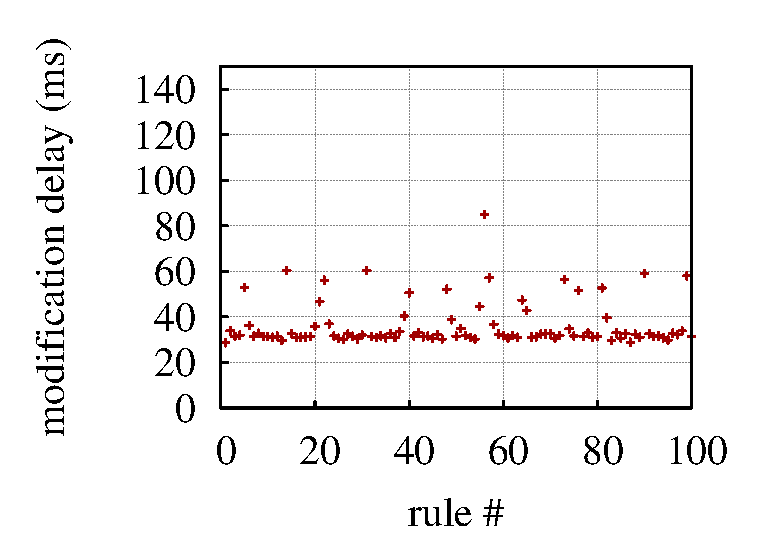
\includegraphics[width=.5\linewidth]{./figs/jan27_bcm_mod_same_burst_100_imc.eps}}\hfill
%\subfloat[burst size 100, increasing priority.\label{fig:bcm_mod_incr_burst_100}]
%  {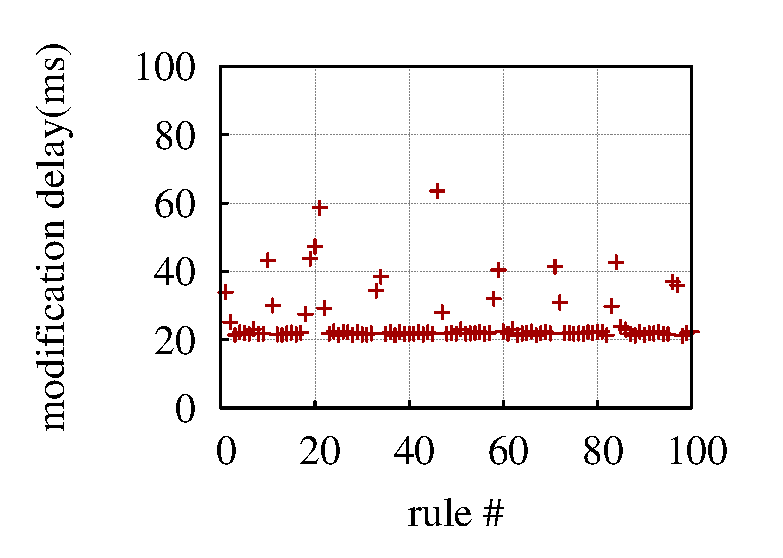
\includegraphics[width=.24\linewidth]{./figs/jan27_bcm_mod_incr_burst_100.eps}}\hfill
%\subfloat[burst size 100, decreasing priority.\label{fig:bcm_mod_decr_burst_100}]
%  {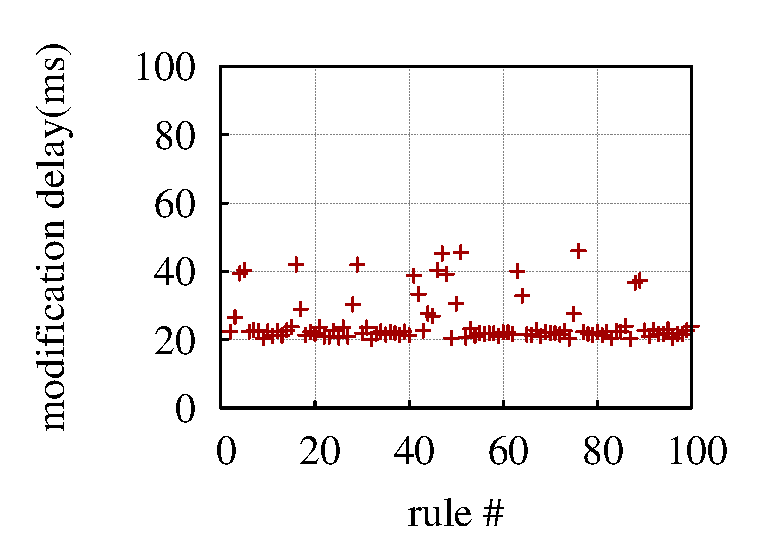
\includegraphics[width=.24\linewidth]{./figs/jan27_bcm_mod_decr_burst_100.eps}}\hfill
\subfloat[200 rules in table \label{fig:bcm_mod_same_burst_200}]
  {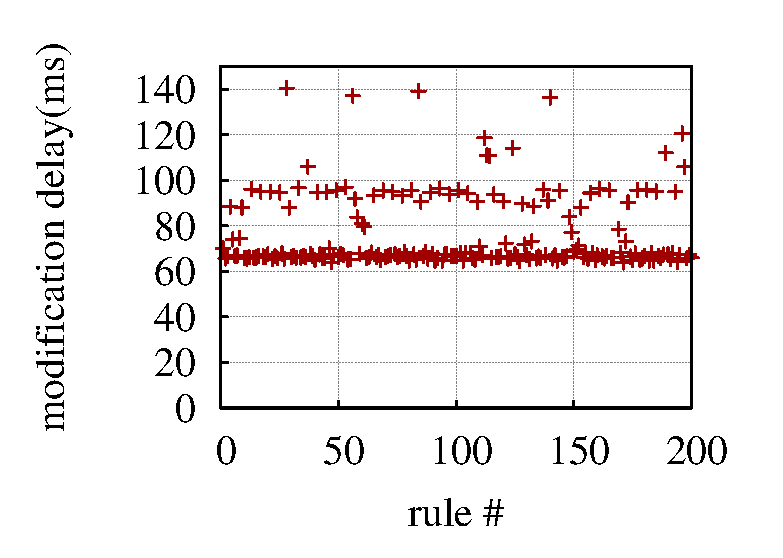
\includegraphics[width=.5\linewidth]{./figs/jan27_bcm_mod_same_burst_200.eps}}
\compactcaption{{\bf \BroadcomOne} per-rule {\bf mod.} latency, same priority}
\label{fig:occupancy-broadcom-modify}
\end{figure}
 
Per-rule modification delay for \BroadcomOne when $S=100$ and $S=200$ are shown in
\figsref{fig:bcm_mod_same_burst_100}{fig:bcm_mod_same_burst_200}, respectively. We
see that the per-rule delay
is more than 30 ms for $S=100$. When we double the number of rules,
$S=200$, latency doubles as well. It grows
linearly with $S$ (not shown). Note that
this latency is much higher than the corresponding
insertion latency (3.12ms per rule) (\S\ref{s:meas_insert}).
%\fixme{IBM added}
\IBM's per-rule modification latency is also affected significantly by the table occupancy---
the per-rule modification latencies for $S=100$ and $S=200$ are 18.77ms and 37.13ms, respectively.
 
\iffalse
\begin{figure}[!tb]
  \centering \subfloat[100 rules in table \label{fig:intel_mod_same_burst_100}]
  {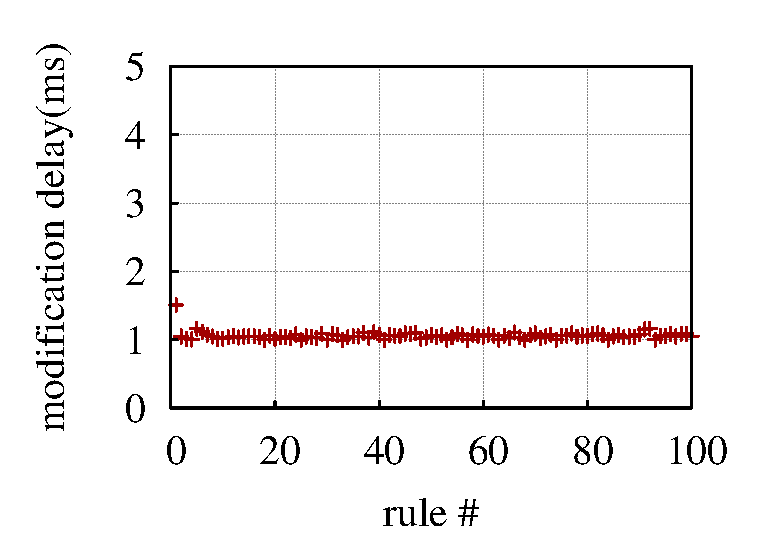
\includegraphics[width=.5\linewidth]{./figs/jan27_intel_mod_same_burst_100.eps}}\hfill
%\subfloat[burst size 100, increasing priority.\label{fig:intel_mod_incr_burst_100}]
%  {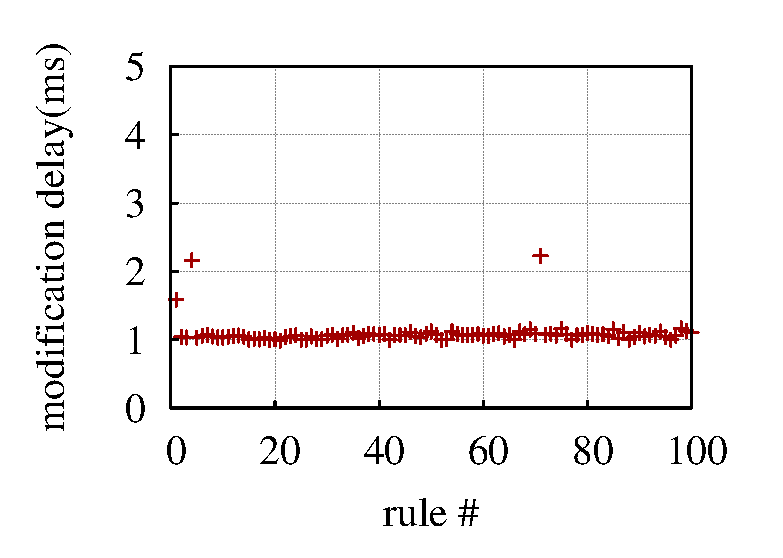
\includegraphics[width=.24\linewidth]{./figs/jan27_intel_mod_incr_burst_100.eps}}\hfill
%\subfloat[burst size 100, decreasing priority.\label{fig:intel_mod_decr_burst_100}]
%  {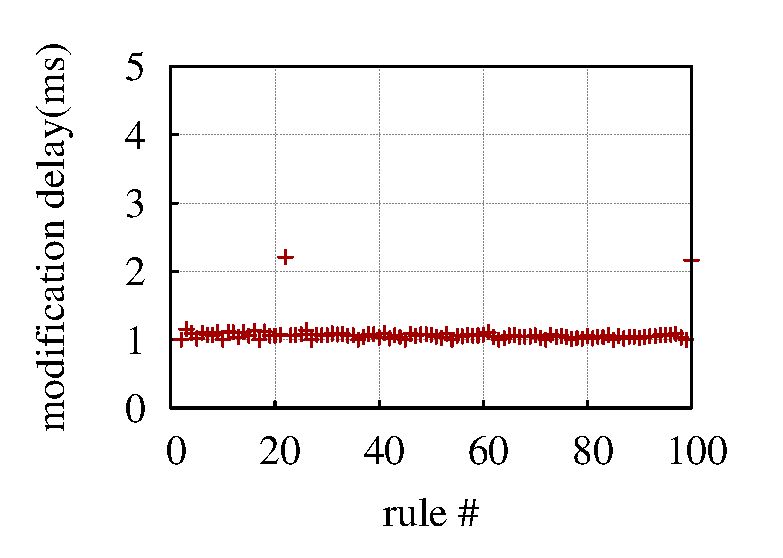
\includegraphics[width=.24\linewidth]{./figs/jan27_intel_mod_decr_burst_100.eps}}\hfill
\subfloat[200 rules in table \label{fig:intel_mod_same_burst_200}]
  {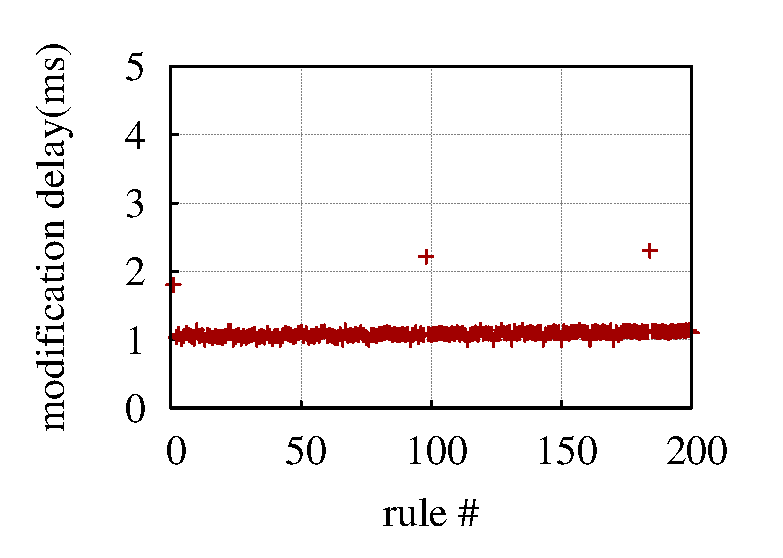
\includegraphics[width=.5\linewidth]{./figs/jan27_intel_mod_same_burst_200.eps}}
\compactcaption{{\bf \Intel} per-rule {\bf mod.} latency, same priority}
\label{fig:occupancy-intel-modify}
\end{figure}
\fi
%The results for $S=100,200$ for Intel are shown in
%Figure~\ref{fig:occupancy-intel-modify}. 
%Sourav commented
%For Intel, the modification delay for $S=100,200$ is around 1 ms
%(standard deviation 0.06) for all modified rules, similar to insertion
%in Figure~\ref{fig:priority-intel-insert}.
%delay with same priority,  in contrast with
%\BroadcomOne. 
% the modification delay is around 1 ms, which is the same as
% the insertion delay when all rules have same priority
% (\S\ref{s:meas_insert}).
% The results are the same for higher values of
% $S$.

In contrast, \Intel and \BroadcomThree  have lower modification delay,
and it does not vary with table occupancy. For \Intel (\BroadcomThree) the
per-rule modification delay for both $S=100$ and $S=200$ is around 1 ms (2ms)
for all modified rules, similar to (2X more than) same priority insertion delay. 

%\aditya{I changed the previous sentences. Check!!}
%%  For \BroadcomThree the average modification delay (standard deviation) for $S=100$ and $S=200$ is 2.19 (1.82) and 2.95 (2.29) respectively.
%For \BroadcomThree the modification delay is highly variable and is 
%related with table occupancy. For example, modifying 200 %rules in a table with 200 and 500 rules takes 449 and %4984 msec respectively. 

\minisection{Rule Priority} We conduct two experiments on each switch to
study the impact of rule priority. In
each experiment, we insert $B$ rules into an empty table ($S = 0$). In the 
{\em increasing} priority experiments, the rules in the table each have a
unique priority, and we send back-to-back modification requests for
rules in increasing priority order. We do the opposite in the {\em
decreasing priority} experiment. We vary $B$.%  across
% experiments. Note that the {\em same priority} experiment here is
% exactly the same as the table occupancy experiment above; hence we
% omit it.

\begin{figure}[!tb]
\centering
%\subfloat[burst size 100, same priority.\label{fig:bcm_mod_same_burst_100}]
%  {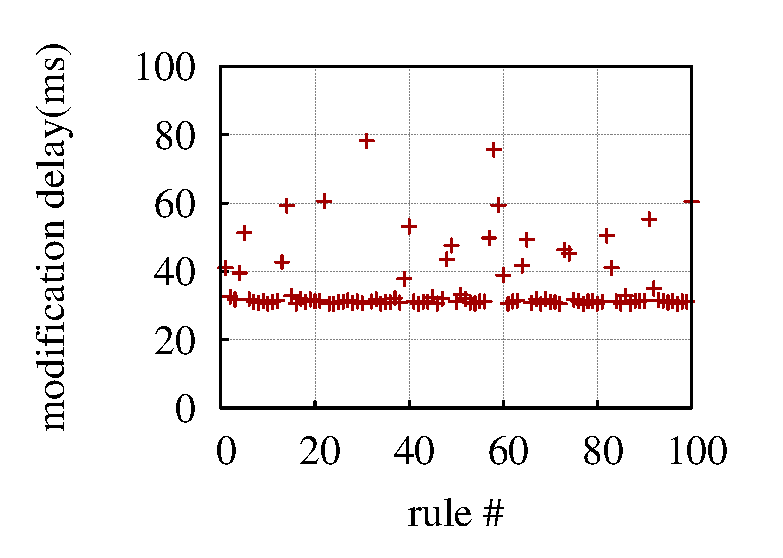
\includegraphics[width=.5\linewidth]{./figs/jan27_bcm_mod_same_burst_100.eps}}\hfill
\subfloat[burst size 100, incr. priority\label{fig:bcm_mod_incr_burst_100}]
  {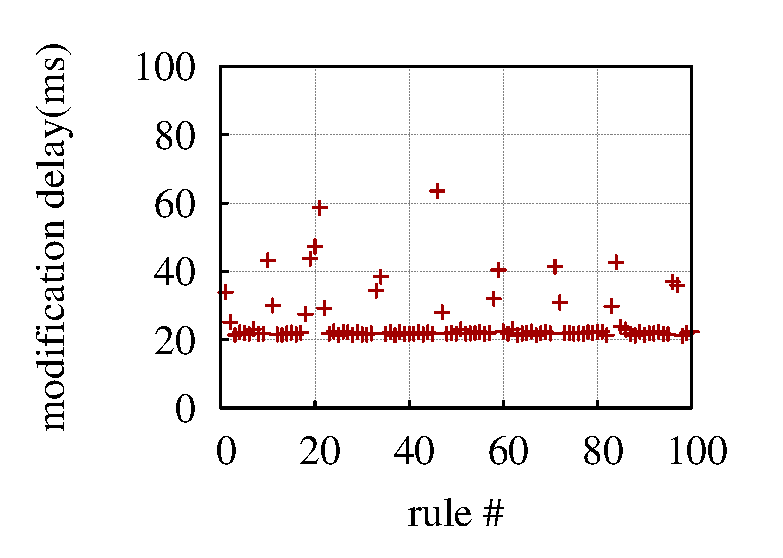
\includegraphics[width=.5\linewidth]{./figs/jan27_bcm_mod_incr_burst_100.eps}}\hfill
\subfloat[burst size 100, decr. priority\label{fig:bcm_mod_decr_burst_100}]
  {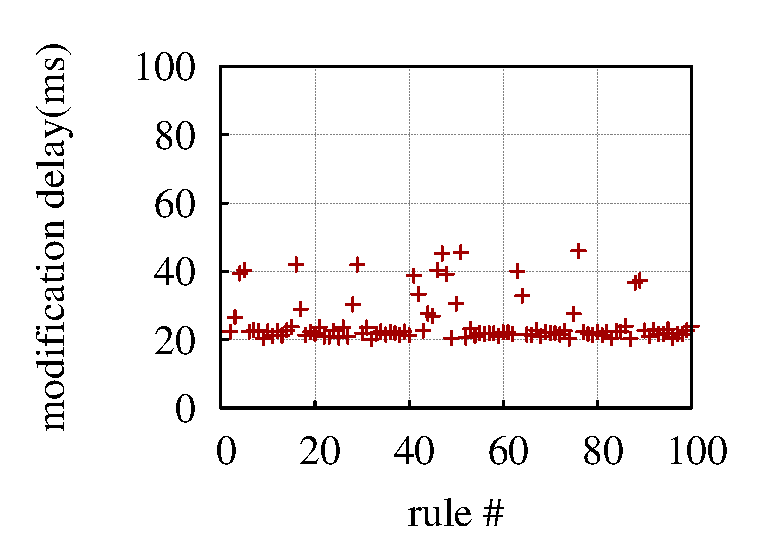
\includegraphics[width=.5\linewidth]{./figs/jan27_bcm_mod_decr_burst_100.eps}}\hfill
%\subfloat[burst size 200, same priority.\label{fig:bcm_mod_same_burst_200}]
%  {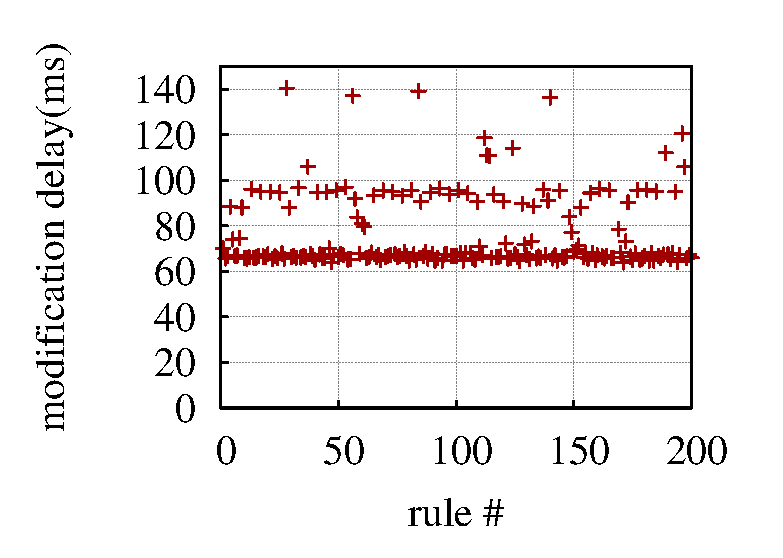
\includegraphics[width=.5\linewidth]{./figs/jan27_bcm_mod_same_burst_200.eps}}
\compactcaption{{\bf \BroadcomOne} priority per-rule {\bf modification} latency}
\label{fig:priority-broadcom-modify}
\end{figure}

%\emph{\BroadcomOne: increasing/decreasing priority.}
\figsref{fig:bcm_mod_incr_burst_100}{fig:bcm_mod_decr_burst_100} show the results for the increasing and decreasing priority experiments, respectively, for
$B=100$ on \BroadcomOne. In both cases, we see: (1) the per-rule modification delay is similar
across the rules, with a median of 25.10ms and a standard deviation of
6.74ms, and (2) the latencies are identical across the experiments. 
We similarly observe that priority does not affect modification delay in
\BroadcomThree, \Intel and \IBM (not shown).
% Again, the
% latencies are  much larger than insertion with same priority, 25 ms vs 3 ms.
%\aditya{this is not true! bcm insertion latencies are also high!} 
%li: add same priority, fixed, right?
%We observed that the latencies grew with $B$ for both experiments.
% increasing and decreasing
% priority experiments.

% Figure~\ref{fig:priority-broadcom-modify}-d shows the results for
% $B=200$, and again the per rule latency is about twice as high as that
% for $B=100$. 
% % per-rule modification delay for 200 rules has a median 60 (xx) ms and
% % standard deviation xx. The modification time is significant impacted
% % by the number of rules in the table.

% \emph{Broadcom: decreasing priority.}  We modify in both increasing rule
%   priority and decreasing rule priority. As shown in
%   Figure~\ref{fig:priority-broadcom-insert}-b,c, the per rule modification delay
%   is not affected by rule priority. Their median delay is xx and xx respectively
%   with standard deviation xx and xx.

%We next describe our measurement results on Intel. 
\iffalse
\begin{figure}[!tb]
\centering
%\subfloat[burst size 100, same priority.\label{fig:intel_mod_same_burst_100}]
%  {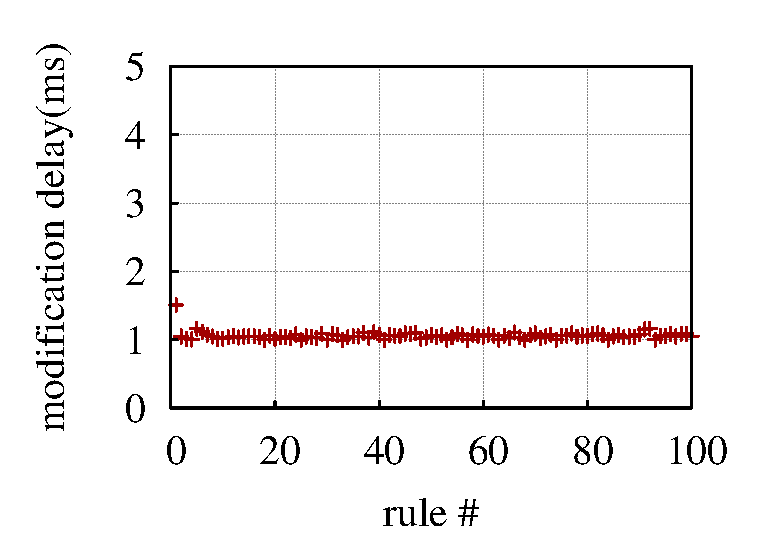
\includegraphics[width=.5\linewidth]{./figs/jan27_intel_mod_same_burst_100.eps}}\hfill
\subfloat[burst size 100, increasing priority.\label{fig:intel_mod_incr_burst_100}]
  {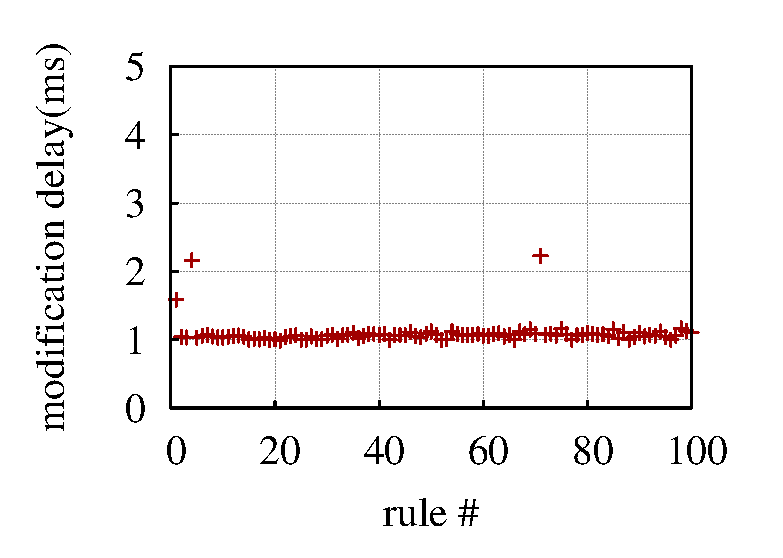
\includegraphics[width=.5\linewidth]{./figs/jan27_intel_mod_incr_burst_100.eps}}\hfill
 \subfloat[burst size 100, decreasing priority.\label{fig:intel_mod_decr_burst_100}]
  {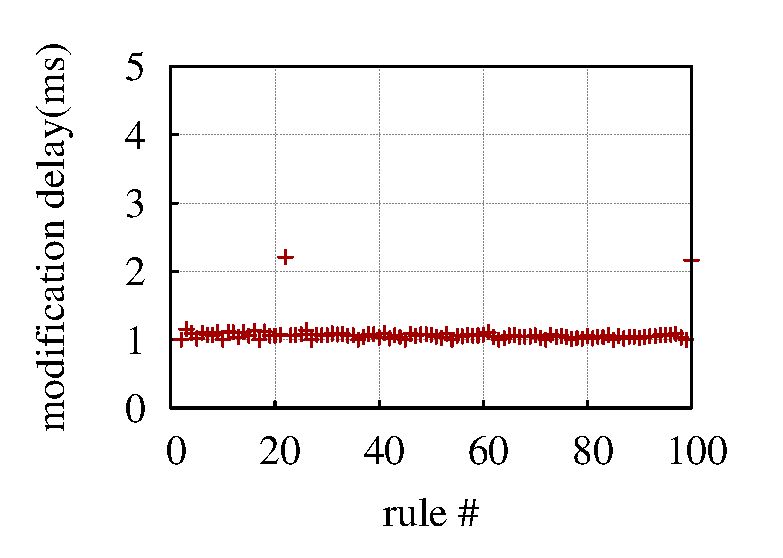
\includegraphics[width=.5\linewidth]{./figs/jan27_intel_mod_decr_burst_100.eps}}\hfill
%\subfloat[burst size 200, same priority.\label{fig:intel_mod_same_burst_200}]
%  {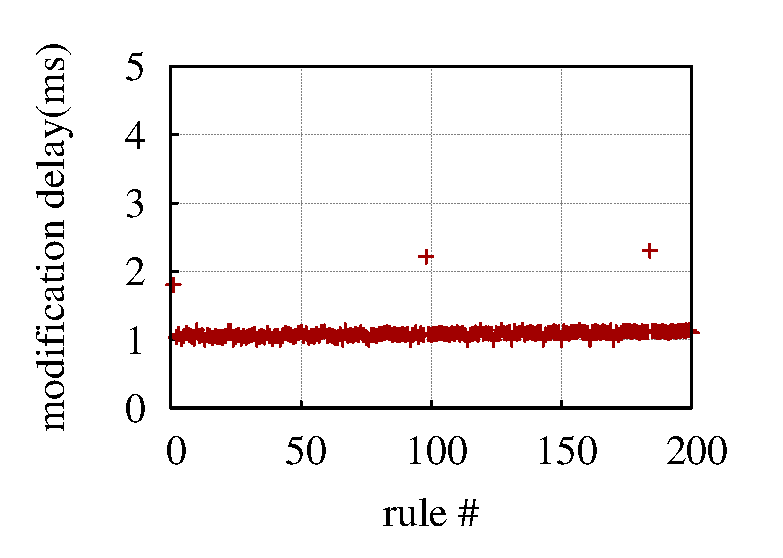
\includegraphics[width=.5\linewidth]{./figs/jan27_intel_mod_same_burst_200.eps}}
\caption{{\bf Intel} priority per-rule {\bf modification} latency results}
\label{fig:priority-intel-modify}
\end{figure}
\fi

%{\em Intel increasing/decreasing priority.} 
%Figure~\ref{fig:priority-intel-modify} shows the result for $B=100$ on
%Intel.
% , similar to insertion delay without
% priority.  We also tried other B values and the results are similar (omitted for brevity).


\minisection{Summary and root causes}
%Given our table occupancy and rule priority results, 
We conclude that the per-rule modification latency on \BroadcomOne and \IBM is 
impacted purely by table occupancy, not by rule priority structure.
For \BroadcomThree and \Intel, the per-rule modification delay 
%is 1 ms respectively 
is independent of rule priority, table occupancy, and burst size;
\BroadcomThree's per-rule modification delay is 2X higher than insertion.
%For \BroadcomThree, the modification delay is independent of rule priority but 
%is highly variable and is          
%related with table occupancy. The root cause of the variable and larger modification delay on 
%\BroadcomOne and \BroadcomThree is that modification involves insertion and deletion operation and it causes
%TCAM reorganization.

%We observe that flow rule priority do
%not impact modification delay. Modification delay in \BroadcomOne and \BroadcomThree is a
%function of table occupancy, whereas this is not the case for Intel where modification is as fast as insertion. 
Conversations with Broadcom indicated that TCAM modification should ideally be fast and independent of table size, 
so the underlying cause appears to be less optimized switch software in \BroadcomOne. Indeed, our measurements with \BroadcomThree show that this issue has (at least partly) been fixed.

% However, for Broadcom, the modification delay is much higher
% than rule insertion delay with same priority. For Intel, the modification delay
% is similar to rule insertion delay with same priority. 

% \aditya{missing causes!}


% LocalWords:  pre Broadcom

\subsubsection{Deletion Latency}
We now estimate the impact of rule deletions.
We use bursts of operations as before.
Denote
$T(r_i)$ as the first time we stopped observing packets matching rule $r_i$
from the intended port of the rule action. We define deletion latency
as $T(r_i)-T(r_{i-1})$.

\begin{figure}[!tb]
\centering
\subfloat[100 rules in table \label{fig:bcm_del_same_burst_100}]
  {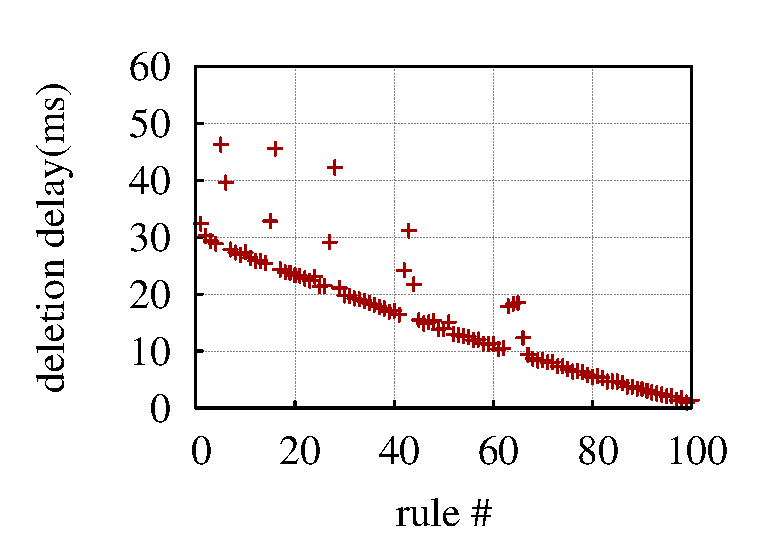
\includegraphics[width=.50\linewidth]{./figs/jan27_bcm_del_same_burst_100.eps}}\hfill
%\subfloat[burst size 100, increasing priority.\label{fig:bcm_del_incr_burst_100}]
%  {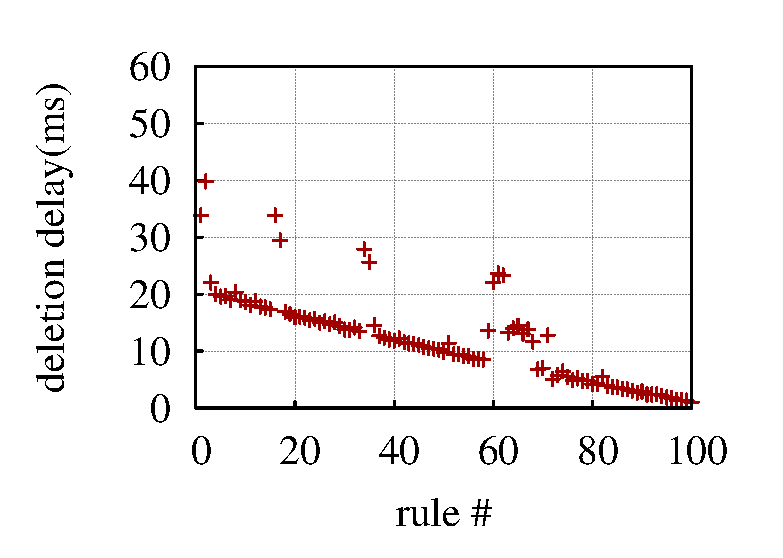
\includegraphics[width=.30\linewidth]{./figs/jan27_bcm_del_incr_burst_100.eps}}\hfill
\subfloat[200 rules in table \label{fig:bcm_del_same_burst_200}]
  {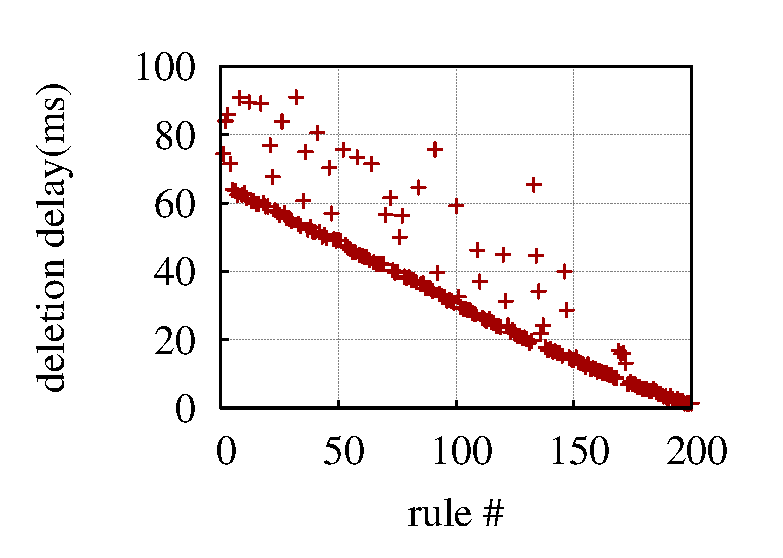
\includegraphics[width=.50\linewidth] {./figs/jan27_bcm_del_same_burst_200.eps}}
\compactcaption{ {\bf \BroadcomOne} per-rule {\bf del.} latency, same priority}
\label{fig:occupancy-broadcom-deletion}
\end{figure}

\begin{figure}[!tb]
\centering
\subfloat[100 rules in table\label{fig:intel_del_same_burst_100}]
  {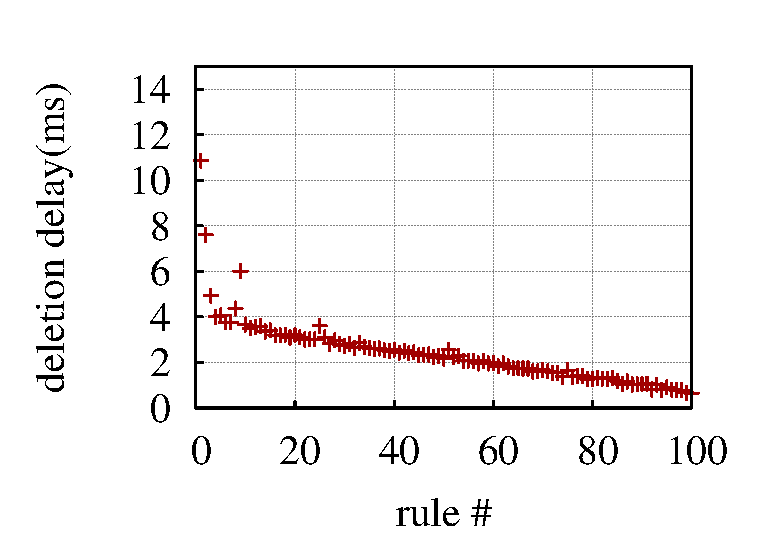
\includegraphics[width=.50\linewidth]{./figs/jan27_intel_del_same_burst_100.eps}}\hfill
%\subfloat[burst size 100, increasing priority.\label{fig:intel_del_incr_burst_100}]
%  {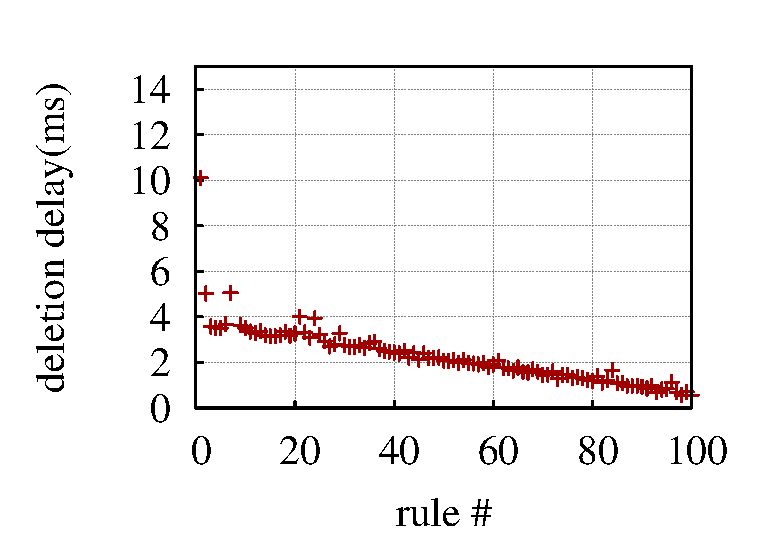
\includegraphics[width=.30\linewidth]{./figs/jan27_intel_del_incr_burst_100.eps}}\hfill
\subfloat[200 rules in table \label{fig:intel_del_same_burst_200}]
  {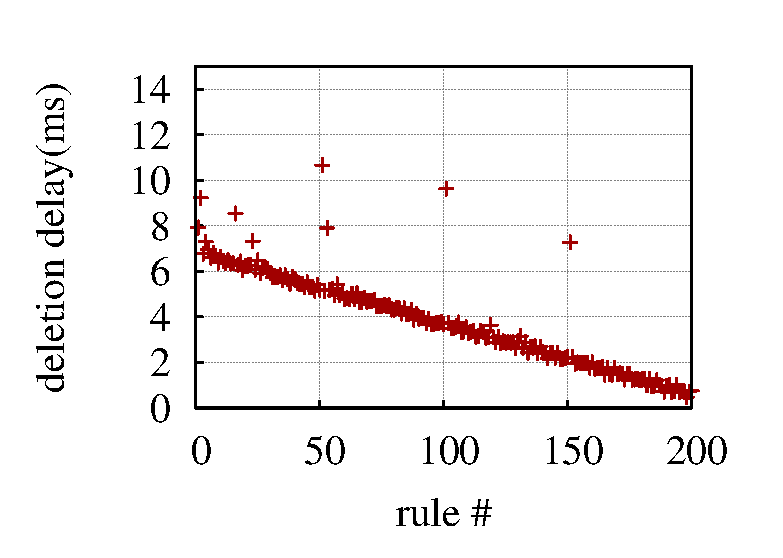
\includegraphics[width=.50\linewidth]{./figs/jan27_intel_same_burst_200.eps}}
\compactcaption{{\bf \Intel} per-rule {\bf del.} latency, same priority}
\label{fig:occupancy-intel-deletion}
\end{figure}

\minisection{Table Occupancy} We pre-insert $S$ rules into a switch, all with
the same priority. We then delete one rule at a time, sending deletion
requests back-to-back. The results for \BroadcomOne at $S=100$ and $S=200$
are shown in \figsref{fig:bcm_del_same_burst_100}{fig:bcm_del_same_burst_200},
respectively. We see that per rule deletion delay decreases as the table occupancy drops. We see a similar trend for Intel (\figsref{fig:intel_del_same_burst_100}{fig:intel_del_same_burst_200}) and \BroadcomThree (figure not shown).

%  and
% ~\ref{fig:occupancy-intel-deletion}, the per rule deletion delay
% decreases as the table occupancy drops.


\begin{figure}[!tb]
\centering
% \subfloat[burst size 100, same priority.\label{fig:bcm_del_same_burst_100}]
%   {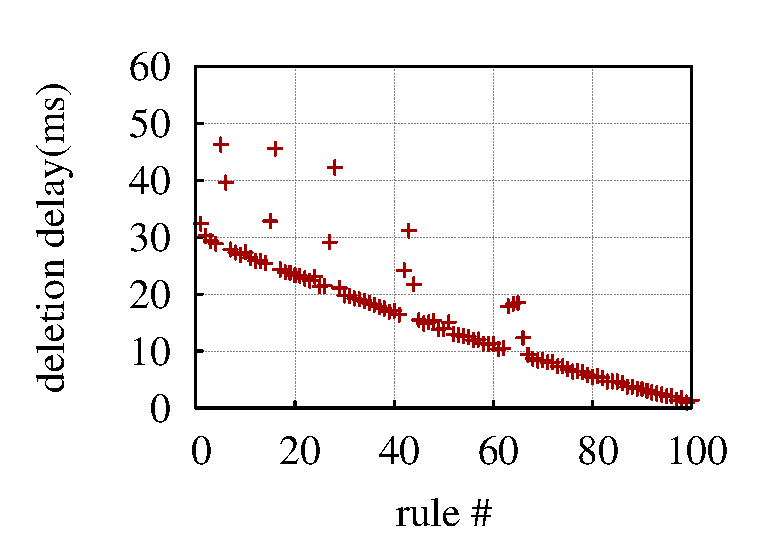
\includegraphics[width=.30\linewidth]{./figs/jan27_bcm_del_same_burst_100.eps}}\hfill
\subfloat[increasing priority\label{fig:bcm_del_incr_burst_100}]
  {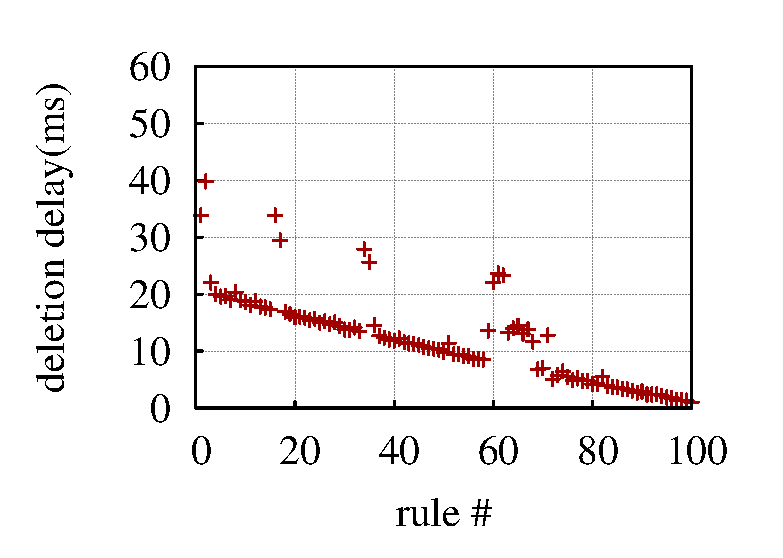
\includegraphics[width=.50\linewidth]{./figs/jan27_bcm_del_incr_burst_100.eps}}\hfill
\subfloat[decreasing priority\label{fig:bcm_del_decr_burst_100}]
  {\includegraphics[width=.50\linewidth]{./figs/jan27_bcm_del_decr_burst_100.eps}}
\compactcaption{{\bf \BroadcomOne} priority per-rule {\bf del.} latency, 
    B=100}
\label{fig:priority-broadcom-deletion}
\end{figure}

\begin{figure}[!tb]
\centering
%\subfloat[burst size 100, same priority.\label{fig:jan27_intel_del_same_burst_100}]
%  {\includegraphics[width=.24\linewidth]{./figs/jan27_intel_del_same_burst_100.eps}}\hfill
%\subfloat[burst size 100, increasing priority.\label{fig:jan27_intel_del_incr_burst_100}]
%  {\includegraphics[width=.24\linewidth]{./figs/jan27_intel_del_incr_burst_100.eps}}\hfill
%\subfloat[burst size 100, decreasing priority.\label{fig:jan27_intel_del_decr_burst_100}]
%  {\includegraphics[width=.24\linewidth]{./figs/jan27_intel_del_decr_burst_100.eps}

% \subfloat[burst size 100, same priority.\label{fig:intel_intel_del_same_burst_100}]
%   {\includegraphics[width=.30\linewidth]{./figs/jan27_intel_del_same_burst_100.eps}}\hfill
\subfloat[increasing priority\label{fig:intel_del_incr_burst_100}]
  {\includegraphics[width=.50\linewidth]{./figs/jan27_intel_del_incr_burst_100.eps}}\hfill
\subfloat[decreasing priority\label{fig:intel_del_decr_burst_100}]
  {\includegraphics[width=.50\linewidth]{./figs/jan27_intel_del_decr_burst_100.eps}}

\compactcaption{{\bf Intel} priority per-rule {\bf del.} latency, B=100}
\label{fig:priority-intel-deletion}
\end{figure}


\minisection{Rule Priorities} We start with $B$ existing rules in the switch, 
and delete one rule at a time
%,``with'' and ``without priority''. In the former case, 
%we delete rules 
in increasing and decreasing priority order. 
For \BroadcomOne (\figref{fig:priority-broadcom-deletion}), \BroadcomThree
(figure not shown) and Intel (\figref{fig:priority-intel-deletion}), deletion 
is not affected by the priorities of rules in the table or the order of
deletion. %\aaron{Where are the without priority results?}


\minisection{\bf Root cause} Since deletion delay decreases with rule number 
in all cases, we conclude that deletion is incurring TCAM reordering.
% We observe that rule priority pattern does not affect deletion delay for both
% Broadcom and Intel. However, flow table occupancy affects deletion delay
% significant. Deletion delay can be much higher than insertion delay with same
% priority. 
% This seems to indicate that deletion incurs TCAM reordering in all
% cases in both switch architectures.
We also observe that processing rule timeouts at the switch does not
noticeably impact \flowmod operations. Given these two observations, we
recommend allowing rules to time out rather than explicitly deleting them, if
possible.

% LocalWords:  pre Broadcom TODO butbound TCAM



%\section{Mazu Overview}
\begin{figure}
\centering
%\begin{minipage}{.45\textwidth}
  \centering
  \includegraphics[width=0.25\textwidth]{figs/Mazu_7.pdf}
  %Mazu_frame_new.png}
\caption{Mazu framework}
\label{fig:framework}
\end{figure}

Our goal is to develop a general set of techniques that an SDN network can
employ to overcome the impact of the latencies described above on key management
applications. Ideally, the techniques must work across all applications,
switches and deployment settings. To this end, we present a new controller framework called Mazu (Figure~\ref{fig:framework}).

To eliminate all inbound delays, and some outbound delays
(namely, \packetout procesing), we introduce a proxy that generates \packetin
and processes \packetout messages on behalf of one or more switches.

%The Mazu controller implements a number of modules. The first, i.e., proxy,
%handles inbound processing. We show that the proxy can in fact eliminate all
%inbound delays (\S\ref{s:inbound}). 

Because the underlying causes of outbound delays are tightly linked with
switch software and hardware, we can hope at best to mitigate these
latencies. The remaining modules achieve this. The key insight underlying them
all is to organize the \flowmod\ input provided to switches such that the
aggregate rule installation latency experienced by the application is minimized,
given the underlying latency causes. 

% a framework that 
% previous section on various key management applications. We wish to
% develop a general set of approaches that work across most if not all
% applications and deployment settings. % Our ultimate goal is to ensure
% % applications meet the goals they were designed for as effectively as
% % possible.
% Ideally, the approaches we propose must avoid the latencies altogether. We show that this is possible to achieve for inbound delay. 


% % We present, Mazu, a systematic framework that addresses latency problems
% % comprehensively. 
% % %how a network that has
% % %deployed SDN can overcome the impact of the latencies described in the
% % %previous section on various key management applications. 
% % Our goal is to develop a general set of approaches that work across most if not
% % all applications and deployment settings. 
% %Our ultimate goal is to
% %ensure applications meet the goals they were designed for as
% %effectively as possible.
% As shown in Figure~\ref{fig:framework}, \aditya{not sure we
%   want to show proxy inside the controller, as we argue in the next
%   sectio that this is a bad dea. FIXME}

{\em Flow engineering} is an application-dependent module that computes routes
that spread flows across paths in a network, so as to minimize rule
installation latency by controlling rule displacement at any switch, while
adhering to network objectives (\S\ref{s:floweng}).
{\em Rule offloading} takes the set of rules to be installed at any ingress
switch as an input (these could be rules computed by the flow engineering step
above), and carefully offloads/spreads subsets of these rules to downstream
switches/routers having sufficient capacity to hold the rules
(\S\ref{s:offload}). 
By virtue of reducing the installation latency per switch and enabling parallel 
execution of updates, these techniques ensure rule update tasks finish much
faster.  

% Together these techniques 

% This provides two advantages: (a) it further reduces
% the number of rules installed at any switch. (b) The updates can be
% executed in parallel thereby improving the overall time for insertion.

 {\em Rule Reordering} module reorders the rules to be installed at a
 switch (e.g., those computed by rule offload scheme above) into a
 sequence that is optimal with respect to the switch's hardware table
 management scheme. This helps further control rule installation
 latency (\S\ref{s:optimal}). 

%This
% techniques mitigates the impact of step 3.

%\aditya{took out multipath probing for now}
%\aditya{cut this out: In multipath probing, the controller sets up multiple
%  paths in parallel so that data plane packets can be 
% switched in hardware as soon as one path completes its setup.  This
% mechanism deals with unexpected delays imposed by switch CPU (e.g.,
% due to CPU  processing
% of other tasks such as polling statistics) and hardware (e.g., due to
% TCAM reorganization). }

% wherein the controller
% probes a collection of otherwise equivalent paths and
% opportunistically installs rules on the path with the lowest likely
% end-to-end installation latency. Whereas the above
% steps apply to proactive batch installation of rules, this step is
% designed for reactive insertion of rules. In such
% situations, paths have to be set up quickly on demand and as such the
% management applications may be unable to control other actions
% switches may be simultaneously executing, such as replying to \pollstats\ or flushing out timed-out rules. \aditya{check this last
%   sentence. also check the font used for the command.}
 
% The multipath probing
% module sets up multiple paths in parallel. Data plane packets can flow through as
% soon as the first path completes installation. This handles variable delay in
% switch updates. The rule offloading module offloads rules to neighboring
% switches to reduce latency. The optimal rule update module tries to update
% switches as fast as it can.
\iffalse
\subsection{Inbound delay}
%We present a novel middlebox that isolates the processing of packet\_in messages
%from other actions on the switch, thereby almost eliminating t\_in. A network
%operator can deploy such middleboxes adjacent to ingress switches in her
%network.
For packet\_in processing, 
To elaborate, a packet typically follows these steps at the switch: 1)
arrives at port and is processed by ASIC, 2) ASIC decides to send "to
CPU" across PCI bus, 3) OS interrupt is raised and ASIC SDK gets
packet, 4) switch-side openflow agent wakes up, processes packet, and
puts on socket to controller.

%a packet typically follows the following steps at the
%switch: 1) arrives at the switch port and PHY, 2) is processed by ASIC, 3) ASIC decides to send "to CPU", 4)
%packet goes across PCI bus to CPU, 5) OS interrupt is raised and handled, 6)
%ASIC SDK gets packet and fires it off to a dispatch hook, 7) switch-side
%openflow agent wakes up, pro- cesses packet, and puts on socket to
%controller. 

Steps 1 to 4 are typically quite fast. The latencies we observe are mainly due to
steps 5 to 7. Earlier measurements show that steps 5 to 7 are slow due to
unoptimized switch implementations. Our measurements indicate that the newer
switches we measured have better implementations of these steps, but latency
arises nevertheless due to contention between simultaneous processing of
packet\_in messages along- side packet\_out flow\_mod and flow statistics
polling messages being received from the controller. 
 
To overcome the inbound latency entirely the key insight we leverage is to
physically decouple the switch's handling of packet\_in and packet\_out messages
from flow\_mod messages. We punt all packet\_in message generation and packet\_out
processing to a separate optimized processing unit, e.g., simple middlebox,
adjacent to the switch. We establish a (short) label-switched path between the
switch and its corresponding middlebox. The switch continues to have a control
channel to the controller (an SSL connection); in addition, we establish a
control channel (SSL) between the middlebox and the controller. The controller
must be aware of the middlebox's presence and must associate it with the
relevant switch. 

To exercise the middlebox, we insert a default low priority rule in the
switch; this helps redirect all unmatched packets on the label-switched path
to the middlebox. The middlebox generates the necessary
packet\_in messages and forwards them on its control channel to the
controller. The controller sends packet\_out messages to the middlebox; the
middlebox process the message and forwards the corresponding data packet to the
switch for further forwarding to the eventual destination. 
%flow\_mod messages directly to the switch. 

\subsection{Outbound delay}
%Ideally, the approaches we propose must avoid the latencies altogether
%to ensure that the applications can be supported effectively. We show
%that this is possible to achieve for inbound delay. However, 
Because
the underlying causes of outbound delays are tightly linked with how
the switches processes and stores forwarding rules, we can hope at
best to mitigate these latencies, and complete avoidance is
impossible. We develop a multi-step approach to maximally mitigate the impact on
outbound delay of various factors we have discovered.

First, we propose flow engineering that attempts to control the aggregate number
of rules inserted at any switch while adhering to the objectives of the
application(s) running. As such, this technique has to be implemented within the
application itself, although, we present a general framework for introducing
flow engineering into a given SDN applications. Flow engineering helps
upper-bound the aggregate impact of steps 1 and 2 above on any given switch. 

Second, we propose rule offload, where a subset of the rules to be installed at
a switch are carefully offloaded to downstream switches/routers having
sufficient capacity to hold the rules. This provides two advantages: (a) it
further reduces the number of rules installed at any switch. (b) The updates can
be executed in parallel thereby improving the overall time for insertion. 

Third, we propose priority ordered insertion, where the rules computed for
insertion at a switch are reordered into a sequence that is optimal with respect
to the switch's hardware table management scheme. This techniques mitigates the impact
of step 3. 

Fourth, for a given flow, we can setup multiple paths in parallel. Data plane
packets can go through as soon as the first path completes setup.
\fi

%\section{Handling Inbound Delay}
\label{s:inbound}

\iffalse
\aditya{this section talks about packetout, but our measurements don't
  cover them}

Recall the 3 steps I1--I3 taken by a switch to process \packetin described in
Section XXX. Step I1 is typically quite fast. The latencies we observe is mainly
due to steps I2 and I3. Earlier measurements~\cite{flowvisor} show that these
steps are slow due to unoptimized switch implementations. Our measurements
indicate that the newer switches we measured have better implementations of
these steps, but latency arises nevertheless due to contention between
simultaneous processing of \packetin\ messages alongside \flowmod\ and
\pollstats\ commands received from the controller. \aditya{this can go at the
  end of section 3} 
\fi
%\keqhe{please check below}
\iffalse
Reactive flow path setup enables fine-grained visibility and more programmability of the network. 
As we have mentioned, mobility support is one appealing reactive application enabled by SDN. 
When mobile users move across the networks, the SDN controller can setup paths in an on-demand manner. 
Another promising reactive application is security. Network administrator can program the network devices and 
let the packets matching certain fields go to the SDN controller. For example, all DNS traffic can be redirect to 
the SDN controller and the controller checks whether the flows are trying to access some malicious websites on a blacklist.
\fi

\iffalse
\sourav {Check}
The applicability of some important reactive applications like mobility and Dns security as described in section (\S\ref{s:apps}) is impacted by inbound delay.
To overcome the inbound latency, what we propose is to
  physically decouple the switch's handling of \packetin and \packetout messages from \flowmod\ messages. 
%\aditya{we need a picture here} 
We punt all \packetin\ message generation and \packetout\ processing to a
separate optimized processing unit, i.e., a custom proxy, co-located with ingress (edge)
switches in a network; The nice properties introduced by this idea are 
1) reactive path setup packets can avoid the bottleneck ASIC-CPU bandwidth in modern switch systems~\cite{devoflow} because the packet\_in 
and packet\_out packets go through data plane; 2) the switch CPU load is no longer a system bottleneck and 
the interference with proactive path setup is mitigated. As we will demonstrate later, 
the proxy capacity can handle many co-located switches' requests so the cost is reduced 
compared with the solution of getting high end switches with better hardware.

We establish a (short) label-switched path between the switch and its
corresponding proxy. The switch continues to have a control
channel to the controller; the controller associates each switch with its
relevant proxy. Then we insert openflow rules (based on application, e.g, DNS traffic) in the switch; this
redirects at line rate all the packets matching the specified rules 
on the label-switched path to the
proxy. The switch stamps the incoming port ID in the TOS field on the 
packet before label-switching it to the proxy.  The proxy 
%\aditya{check this. i think we need to buffer data plane packets at proxy} 
generates the necessary \packetin\ messages reflecting the
switch's incoming port ID, and forwards them on its control channel to the
controller, and buffers \packetin\ locally (similar to a regular switch).
%This helps the controller know the switch port on which the packet arrived. 
%\aditya{is this correct?}
The controller sends \packetout\ messages to the proxy; the proxy processes the message and forwards the buffered packet corresponding to the \packetin\ back to 
the switch for routing to the eventual destination.  \flowmod\ messages are sent directly to the switch.\fi



Inbound latency can have a pronounced impact on reactive applications such as
those described in \secref{s:apps}. 
To overcome the primary factor contributing to this latency---limited bus
bandwidth between the switch ASIC and CPU (\secref{s:measure_inbound})---we
introduce physically decoupled processing units, i.e., custom proxies, that
generate \packetin and process \packetout messages.

%the contention for
%limited switch CPU and bottlenecked ASIC-CPU bandwidth as the main
%contributors for inbound latency, we introduce physically decoupled optimized
%processing units, i.e., custom proxies that are capable of generating
%\packetin and processing \packetout messages, as a solution to overcome it.

Proxies are co-located with the ingress (edge) switches in the network, and
we establish a (short) label-switched path between each switch and its
corresponding proxy. The switches continue to have a control channel to the
controller. We then insert OpenFlow rules in the switches that forward to
their proxy, at line rates, all packets that would have otherwise required
them to generate \packetin messages. The switches stamp the incoming port ID
in the ToS field of the packets before forwarding them to the proxy; this can
be achieved by installing one rule for each switch port which matches
based on in-port and sets the packet's ToS
field accordingly. The
proxy then generates the necessary \packetin messages reflecting the
switches` incoming port ID, and forwards them on its control channel to the
controller. Similar to a regular SDN switch, the proxy also locally buffers
the packets. The controller sends any \packetout messages to the proxy, which
processes them and forwards the corresponding buffered packets back to the
switch to be routed to their eventual destination. All \flowmod messages are sent
directly to the switch by the controller. 

A single proxy, as we will show in \secref{s:eval_inbound} is capable of
serving multiple switches and is thus cost-effective. We also show that it
drastically reduces inbound latency. As an added benefit, more switch CPU
resources are available for processing \flowmod{s}, polling statistics, etc.
  
%the switch CPU is no longer a system bottleneck and thus the interference with proactive path setup is also mitigated.


%\aditya{please double check this!!} 
 %In effect, the approach avoids the need for steps 3 and 4 on the switch altogether, and isolates and speeds up steps 5--7.

% It is possible to integrate the proxy within the SDN controller
% itself. 
% % The switches uses a dedicated physical port to contact the
% % controller. The controller establishes a label switched path from and
% % to the switch. The default rule installed at the switch forwards
% % unmatched packets to deliver them to the controller \aditya{check
% %   this}.
% %\aditya{rest of the details are same as with MB}
%   This avoids the need for generating \packetin\  messages
%   altogether, and avoids having to deploy proxies in the network.
% % : (1)
% %   Packets sent to the controller may be lost due to congestion
% %   en-route.   The original sender
% %   will
% %   have to retransmit lost packets, which can significantly inflate connection
% %   setup delay. While this problem can also arise with the proxy,
% %   the
% %   likelihood of loss is higher as the controller may be located several hops away.
% %   (2) T
%  But  this scheme imposes high overhead: it sends all full length (MSS
%   sized) unmatched packets to the controller. In contrast \packetin\
%   messages are typically much smaller than MSS, e.g., 128B, and in most switch
%   implementations only one packet \junaid{i am not sure whether this claim(only one packet) is correct or not, at least in openflow 1.0 this is not the case. Am I missing some context ?}is sent while the corresponding
%   flow's data packets are buffered at the switch.  Therefore, we shun this
%   approach. 

%   However, in
%   some deployment
%   scenarios, e.g., where switches don't buffer packets anyway, the added load
%   on the controller and the
%   underlying network may not be significant. \aditya{can someone check
%     this?}

%   Depending on the deployment scenario in question either approach
%   could be employed to avoid inbound delay.

% \aditya{the following is unrelated to the paper}
% \keqhe{ 
% One common misunderstanding of the MB approach is that we need to place a MB for each switch. 
% We need to note that MB can be used by multiple openflow switches in a multiplexing manner. 
% For example, in enterprise networks or campus network, the switches in one building can use one MB.
% Further, there are several additional good properties of the MB approach. 
% The first one is, MB enables higher level network programmability. Additional logic can be implemented in the MB to enable more flexible network control. 
% The second one is security. The previous sections show that the CPU sitting on the  switch is used by tasks such as flow mod message processing, TCAM reordering, 
% flow status polling etc. An adversary can easily start an attack on the openflow switch CPU such that all other tasks on the CPU suffers from poor performance. 
% Our MB approach decouples the reactive packet\_in generation task to a dedicated general-purpose CPU 
% (usually much more powerful than embedded switch CPU) so the attack on switch CPU can be successfully mitigated.
% }

% \aditya{Can multiple switches in a network could share a single
%   proxies to collective process their \packetin\  messages?} 


% The main cause of Inbound [Ingress?] delay is high CPU processing overhead in generating the PACKET\_IN message and simultaneous processing of FLOW\_MOD messages from the controller. We propose a MiddleBox solution that offloads the generation of PACKET\_IN from the switch to a high CPU power MiddleBox.  

% \begin{enumerate} 
% \item Control channel is established via the MB. 
% \begin{itemize}
% \item Switch\_MB control channel: Between Switch and MB
% \item MB\_Controller control channel: Between MB and Controller
% \end{itemize}

% \item Controller inserts a default rule:
% \begin{itemize}
% \item Rule0: Forward unmatched packets to MB
% \end{itemize}

% \item PACKET\_IN message generation is offloaded to the MB
% \begin{itemize}
% \item For each unmatched packet received by the MB(forwarded by the switch), it generates a packet\_in message and sends it to the controller via (MB\_Controller) control channel
% \item The controller sends the packet\_out and flow\_mod message to the MB via  (MB\_Controller) control channel
% \item The MB forwards the packet\_out and flow\_mod message to the switch via  (Switch\_MB) control channel
% \end{itemize}
% \end{enumerate}


%\section{Mitigating the Latency of\newline Programming network state}

The success of many SDN applications hinges on their ability to quickly
program network state. For example:

\minisection{WAN Failover}
When WAN failures occur, an SDN application may want to quickly compute new
paths for flows traversing failed nodes or links, while simultaneously
rerouting other high/low priority flows to avoid hot-spots~\cite{swan}.
However, this requires significant updates to network state at multiple
switches. The longer these updates take, the longer traffic is subject to
congestion and loss. We find that outbound latencies can inflate failure
response time by $\approx$ 20s (\secref{s:evaluation}). 

%\minisection{Failover}
%It is possible that SDN can help mitigate the network-wide impact of
%failures in wide-area networks, reducing both downtime and congestion
%without requiring significant over provisioning. When failures occur,
%the SDN management application can quickly compute new paths for flows
%traversing failed nodes or links, while also simultaneously rerouting
%other high/low priority flows so as to avoid hot-spots~\cite{swan}.
%However, this requires significant updates to network state at
%multiple network switches. The longer these updates take, the longer
%the effect of failure is felt in the form of congestion and drops. We
%find that outbound latencies can inflate the time by nearly 20s
%(\secref{s:evaluation}) putting into question SDN's applicability to
%this scenario. 

\minisection{Intra-Datacenter Traffic Engineering} 
To eliminate hot\-spots and maximize data center performance, an SDN
application may want to reroute traffic subsets at fine
timescales~\cite{hedera}. For example, MicroTE~\cite{microte} leverages the
fact that a significant fraction of ToR-to-ToR traffic (ToR is ``top-of-rack''
switch) is predictable on short time-scales of 1-2s. Thus, MicroTE
frequently computes and updates routes at ToR switches.
% The computed routes may only be effective for 1-2s after which a new sets of
% routes may be more optimal. 
Unfortunately, outbound latencies can cause these updates to take up to 0.5s 
(\secref{s:evaluation}), so traffic that is predictable on 1s timescales is 
optimally routed only half the time.
%Thus, latencies in installing routes can significantly undermine MicroTE's
%effectiveness. Indeed, we find that updating a set of routes at a ToR switch
%in MicroTE can take as long as 0.5s on some SDN switches
%(\secref{s:evaluation}). 

To mitigate the impact of outbound latency, and support the needs of these
and other SDN apps, we propose three immediately deployable
techniques: flow engineering (\FE), rule offload (\RO), and rule reordering
(\RR). This section discusses these techniques in detail; we
evaluate them in \secref{s:evaluation}.

\subsection{Flow Engineering}
\label{s:floweng}

\begin{figure}
\centering
%\begin{minipage}{.45\textwidth}
  \centering
  \includegraphics[width=3.2in]{figs/flow_eng_example.pdf} \compactcaption{Flow 
engineering example, assuming \BroadcomOne. $nL$ = $n$ low priority rules;
$nH$ = $n$ high priority rules; capacity = 1000 rules. Ingress and egress 
tables are empty} 
\label{fig:flow_eng} \end{figure}

SDN applications that perform failure recovery, traffic engineering, or other
forms of routing must quickly compute and setup network paths in order to
satisfy reachability and performance objectives. These applications must often
select one of many possible paths based on congestion, delay, flow table 
occupancy, or other metrics. Unfortunately, a (slightly) more optimal path 
according to these metrics may take significantly longer to setup due to 
outbound latency.

For example, consider an SDN application that seeks to minimize the
imbalance in flow table occupancy~\cite{swan, simple, minlanvcrib}. If such an
application needed to setup routes for 100 flows of high priority $H$ in the
topology shown in Figure~\ref{fig:flow_eng}, it would select the first path
through switch $S_A$ for all flows, thereby equalizing the number of flow
table entries across all switches. However, assuming the switches are
\BroadcomOne, this would require displacing {\em each} of the 100 existing
rules of low priority $L$ in $S_A$ for {\em each} of the 100 new flows,
resulting in a total flow installation time of $\approx$1.5s. In contrast, by
routing only 20 new flows through $S_A$, and dividing the remaining flows
evenly between the paths through $S_B$ and $S_C$, we can keep the same level
of imbalance in flow table occupancy ($S_B$ and $S_C$ each have twice as many
entries as $S_A$), while reducing the total flow installation time to
$\approx$0.3s (assuming rules are installed in $S_A$, $S_B$, and $S_C$ in
parallel). 


%SDN applications typically compute paths between various network
%locations that meet some global objective pertaining to
%performance or security. A common issue considered in most prior works
%on such applications is to deal with limited switch table sizes, by
%picking routes that obey or optimize table space
%constraints~\cite{swan,simple, minlanvcrib}. Unfortunately,
%these techniques do not provide sufficient control over outbound
%delay. 

%\minisection{Minimize maximum flow table occupancy is very suboptimal} 
%For example, consider a simple setting where there are three candidate
%paths between a pair of nodes as shown in Figure~\ref{fig:flow_eng}.
%Each path has one Broadcom switch. The switch on the first path
%has 100 rules of low priority L, whereas the switches on the second
%and third paths each have 400 rules of high priority H. Suppose that a
%hypothetical traffic engineering application has 100 flows of priority
%H to allocate to these paths, and each path is equally preferable
%for a flow.  Existing techniques for table space management would
%assign all flows to the first path to minimize maximum flow table occupancy; but
%our measurements for Broadcom 
%show that {\em each} of these 100 rules will displace
%all the 100 low priority rules in the TCAM, resulting in high
%latencies! Allocating 50 flows each on the
%latter two paths instead results in no rule displacement, and the number of
%rules installed per path will be smaller. Thus, when the flows are installed in
%parallel across the latter two paths, this results in significant reduction in
%installation latency. Based on Figure~\ref{fig:burst-completion-time}, it is about 200 ms
%vs 2 seconds, a 10X difference. 
%%Intel switches have similar issues, but for other priority patterns.
%%li: yes, according Marina's information. Low priority rule displaces high
%%priority rule depending on their location.
%%\aditya{check intel claim}

The goal of {\em flow engineering} (\FE) is to select paths that minimize
installation delay while still satisfying an SDN application's primary path
selection criteria (e.g., flow table occupancy or congestion). Assuming there
are many possible sets of paths $\{\mathcal{P}^i_{obj}\}_i$ that (closely)
satisfy an application's objectives, FE selects the set
$\mathcal{P}^{displace}_{obj,tbl\_sz}$ that minimizes the aggregate
latency impact of rule installations, and any associated rule displacements,
while still obeying flow table space constraints.
%The goal of flow engineering is to select paths across the network
%such that installation delay is minimized. The key insight we use is
%the following: in general, there are many possible sets of paths
%$\{\mathcal{P}^i_{obj}\}_i$ in a network that optimize an SDN
%application's objectives, e.g., optimal capacity and latency. From
%this, flow engineering selects the set
%$\mathcal{P}^{displace}_{obj,tbl\_sz}$ that minimizes the aggregate
%impact of both rule displacement in TCAM as well as the number of rules
%installed at any switch, while obeying table space constraints.
% maximum number of rules installed at any
% switch; thus, we spread rule update load {\em laterally}, helping
% improve outbound latencies.
%
$\mathcal{P}^{displace}_{obj,tbl\_sz}$ can be computed using a two step
optimization:
({\em i}) identify sets of paths that satisfy the SDN application's objective 
function,
%\aaron{What is ``the network's objective function?''}
but do not select the actual
paths to use; ({\em ii}) select paths that minimize aggregate
flow installation time.
%effect of rule displacement and the number of rules to be inserted at any
%switch.  
Unfortunately, the time required to solve the integer linear program
(presented in  \appref{app:floweng}) would
outweigh the latency benefits it seeks provide, so we formulate an
efficient heuristic.
%The detailed optimization formulation is a large integer linear
%program (omitted for brevity) and hence inefficient to solve. Below, we
%discuss a simplifying heuristic in the context of a traffic engineering
%application.

\minisection{Flow Engineering Heuristic}
Our goal is to satisfy a bound $C$ on the time required to install/modify
rules across all switches. 
%We initialize $C$ to a low value.

We represent the network as a graph $G = (V,E)$, where each node is a switch
(or PoP) and each edge is a link (or tunnel). Given a traffic matrix $M$, the
SDN application computes $K$ candidate equal cost paths for each $(u,v) \in
V$, where cost is defined in terms of the application's objective (e.g.,
average link utilization). We assume the application also assigns a priority
$Pri(u,v)$ to each flow $(u,v)$.

%\aaron{This is very specific to the objective of minimizing average link
%utilization; can we make this more generic?} 

We sort the flows in decreasing order of resource demand (e.g., bandwidth) and
iterate through them. For each flow $(u,v)$ in the sorted order, we consider
the corresponding $K$ equal cost paths in decreasing order of resource 
availability; let $P^{1\ldots K}_{(u,v)}$ be the sorted order. If the resource
demand $d_{uv}$ can be satisfied by the path $P^{1}_{(u,v)}$, then we compute
whether installing/updating rules for flow $(u,v)$ along this path violates the
latency bound $C$.

%We do this by modeling the per-switch latency, as well as maximum latency
%on the path:

%We represent the network as a graph \textit{G = (V,E)}, where each node is a
%switch (or PoP) and each edge is a link (or tunnel). Given
%a traffic matrix $M$, the application attempts to route it such that the
%average link utilization is within some bound; the heuristic can be easily
%extended to accommodate other objectives.
%% Our goal to compute routes such that the objective is maximized as well as
%% the cost of installing the necessary rules at switches is minimized. 
%%Our heuristic works by exploring for each source-destination pair
%For each source-destination pair we see, whether a path can accommodate both
%its demand, and the path setup latency  
%%imposed by routing the pair across the path's switches 
%is within some bound. If either is violated, we try the next candidate path.
%
%More precisely, suppose we want to bound the maximum cost of
%installing rules at any switch by some $C$. We start by selecting some
%low value for $C$. We assume that we have computed $K$ candidate equal cost
%paths for each $(u,v) \in V$. Suppose the priority of the $(u,v)$ flow
%is $Pri(u,v)$ at every switch in the network (this is
%typically set by the operator).
%
%We sort the traffic demands in decreasing order and
%iterate through them. For each $(u,v)$ in the sorted order, we
%consider the corresponding $K$ equal cost paths in decreasing order
%of available capacity; let $P^{1\ldots K}_{(u,v)}$ be the sorted order. 
%
%If the demand $d_{uv}$ can be satisfied by the path $P^{1}_{(u,v)}$ within
%the utilization bound, then we compute whether installing the $(u,v)$ path
%violates the rule installation latency bound or not. We do this by modeling
%the per-switch latency, as well as maximum latency on the path:



%\minisection{Per-switch latency}
% Recall that we always install new rules,
%and never do rule modifications and deletions. 
%\aditya{the previous sentence may have to go}
% In doing this, an issue to consider is whether the rule for
% $(u,v)$ at $s$ is modifying an existing forwarding rule for $(u,v)$ at
% $s$ (this would happen if $(u,v)$ was being routed through $s$ before,
% but the next hop from $s$ has now changed) or it is a new rule being
% inserted (this happens if $(u,v)$ was never routed via $s$ before).
% However, recall that our measurements show that modifying a rule is
% much more expensive than inserting a new rule (the former incurs the
% cost of potentially reshuffling the entire existing set of rules at
% the switch, whereas the latter only displaces lower priority rules).
% Therefore, we {\em always insert} a new rule for $(u,v)$, ensuring
% that the rule is of higher priority than the existing rule for $(u,v)$
% in $s$ (if any). 
Given our measurement results, for every switch $s \in P^{1}_{(u,v)}$, we can
model the latency at $s$ due to installing rules for $(u,v)$ as 
$L_s = \max(a, (b +c * Disp_s(Pri(u,v))))$. Here, $Disp_s(Pri(u,v))$ is the 
number of rules at $s$ that will be displaced by the rule for $(u,v)$.
%% the following discussion is not very useful, it seems 
%For the Broadcom switch, this is the number of rules of priority {\em lower}  than $Pri(u,v)$, whereas for the Intel switch
%$Disp_s(Pri(u,v))$ is the number of rules of priority \emph{higher} than
%$Pri(u,v)$ divided by 300. 
%This is a conservative estimate assuming all rules
%are packed in increasing priority of slices (\S\ref{s:meas_insert}).
%\aditya{check intel claim} 
%$Disp_s(Pri(u,v))$ can be easily tracked by the SDN
%controller. In the above, 
$a$, $b$ and $c$ are constants derived from switch
measurements. This model essentially says that if the current rule
does not displace any rules from $s$'s existing table, then it incurs
a fixed cost of $a$; otherwise, it incurs the cost given by $b +c *
Disp_s(Pri(u,v))$. The fixed cost $a$ is the insertion delay without any TCAM
reordering. 

%$a$ is the same whether it is modification or insertion for Intel. For
%Broadcom, since we avoided modification, it represents insertion delay without
%TCAM displacement. 
%\aditya{refer back to the model from
%  the measurement section}

%\minisection{Maximum installation latency} 
Now, $\forall s \in P^{1}_{(u,v)}$, we check if $L_s + CurrentL_s \le C$,
where $CurrentL_s$ is the current running total cost of installing the
rules at $s$, accumulated from vertex pairs considered prior to $(u,v)$ in our
iterative approach.
If this inequality is satisfied, we assign $(u,v)$ to the path
$P^{1}_{(u,v)}$ and move to the next vertex pair. If not,
%meaning that installing the $(u,v)$ route on this path violates the
%maximum cost bound $C$ for some switch on the path, then 
we move to the next candidate path for $(u,v)$, i.e., $P^{2}_{(u,v)}$ and
repeat the process.

If after iterating through all flows once, we have not selected a feasible
path for each flow, then we increase $C$ and start from the beginning.
Alternately, we could do a simple binary search on $C$. 
%li: no space for that.
%\aditya{do we need pseudocode?}

%\aditya{assumption: we have a small number of rules we are adding.
%  otherwise, if we can confirm that the decreasing priority weirdness
%  does not apply for all table occupancies, then we should use that}
%\aditya{seems like bcm is buggy so we may not need the above
%  assumption}

% We assign each edge a cost that is the reciprocal of its current available capacity, and find the 
% minimum cost path for the traffic demand. For finding the minimum cost path, we consider precomputed K equal hop length paths, and find
% the path which gives the minimum cost. As we assign a path for a particular traffic demand, 
% we reassign the cost by decreasing the current capacity by the traffic demand for each edge belonging to the
% min-cost path. The idea is that edges which are more highly utilized will get a higher cost value and so the min-cost path for remaining 
% traffic demands will prefer the edges which are lightly utilized. This way, 
% we minimize the maximum load. We analyze the runtime complexity of the algorithm. 

% 
\begin{table}
\begin{scriptsize}
\begin{tabular}{c|l}
Notation & Meaning \\
\hline
$S$ & Set of all switches
\\$S_{ToR}$ & Set of all ToR switches
\\$\tau_{u}$ & Maximum number of flow entries in the switch $u \forall u \in S$
\\$E$ & Set of all physical links (between two adjacent devices)
\\$C_e$ & capacity of individual links $\forall e \in E$
\\$F_{uv}$ & set of all flows from $u$ to $v$ where $u,v \in S$
\\$P_{uv}$ & Set of paths from device $u$ to device $v$
\\$K _{uv}$ & Number of paths from device $u$ to $v$ where $u,v \in S$ 
\\$P^k _{uv}$ & Set of links of $k^{th}$ path from device $u$ to $v$ where $u,v \in S$
\\$T ^f _{uv}$ & Traffic volume from $u$ to $v$ of flow $f$ where $u,v \in S$
\\$util$ & maximum link utilization
\\$I ^{fk} _{uv}$ & Indicator variable denoting that flow $f$ from $u$ to $v$  takes the $k^{th}$ path.
\\$cost$ & maximum cost of rule installation at any switch
\\$M$ & priority of all new rules being inserted
\\$L_s(M)$ & number of rules at switch $s$ of priority lower than $M$
\\ $a$ & cost of installing a rule it has same priority as rules in table
\\ $b$ & constant factor used in modeling rule displacement cost.
\end{tabular}
\label{tab:notation1}
\caption{Notation used in flow engineering formulation.}
\end{scriptsize}
\end{table}

We explain how flow engineering works for simple traffic engineering SDN
application. We represent
the network as a graph \textit{G
  = (V,E)}, where each node is a switch (or a PoP) and each edge is a physical link (or virtual tunnel). Given a traffic matrix, the application attempts to route it such that the maximum link utilization is minimized. Upon computing routes, the application determines the rules to be installed at individual switches. 

For simplicity, we assume that all the rules to be inserted are of the same priority $M$.  We also assume that the control application knows how many rules in each switch have priority lower than $M$, i.e., $L_s(M)$. This can be easily tracked based on history of rule insertions. The notation we use is shown in Table~\ref{tab:notation1}.


{\bf Step 1 - Network Objective:} In the first step we minimize the
maximum link utilization. Let $T ^f _{uv}$ be the traffic volume
 of flow \textit{f} between $(u,v)$, $P^k _{uv}$ be the set of links on
the $k^{th}$ path between (\textit{u,v}). We use a
binary indicator variable $I ^{fk} _{uv}$ to show whether the flow $f$
is on path $k$ or not.  $K _{uv}$ denotes the number of equal hop
length paths between $(u,v)$. 

We have the following capacity constraint: 

% Following are our two
% constraints. First, The total traffic volume from an edge should not
% exceed its $C_e$ times the link utilization limit, $util$. 

\begin{scriptsize}	
\begin{equation*}
    \sum _{u,v \in S_{ToR},~f \in F_{uv},~k  \in P_{uv}~s.t.~e \in P^k _{uv}} T ^f _{uv} *  I^{fk}_{uv} \leq util \times C_e 
\end{equation*}
\end{scriptsize}	
	
The following ensures each flow $f$ takes a single path:	

\begin{equation*}
    \sum _{k  \in P_{uv}} I^{fk}_{uv} = 1 ,\quad \quad \forall u,v \in S_{ToR},~ f \in F_{uv}
\end{equation*}
 
The objective is to minimize the \textit{util}. Note that we do not
compute paths in this step, just the value of the objective function;
suppose the optimal value is $util^*$.

{\bf Step 2 - New Rule Objective:} In second step, we select routes
so as to minimize the rule installation latencies at any
switch. We allow some slack wrt meeting the utilization objective; denote it by
$\delta$. While the second constraint above remains, the capacity
constraint changes to:
 
% First,  traffic traversing from an edge $e$ does not exceed the $C_e$ multipled by 1 $+$ $\delta$ times the $util^*$. $util^*$ is the maximum link utilization we got from the step 1, and  $\delta$ defines an upper limit on maximum link utilization.

\begin{scriptsize}
\begin{equation*}
    \sum _{u,v \in S_{ToR},~f \in F_{uv},~k  \in P_{uv}~s.t.~e \in P^k _{uv}} T ^f _{uv} *  I^{fk}_{uv} \leq (1 + \delta) \times util^* \times C_e 
\end{equation*}
\end{scriptsize}

% We have a similar constraint as above for   Second constraint is same as step 1.\\
  
% \begin{equation*}
%       \sum _{k  \in P_{uv}} I^{fk}_{uv} = 1 ,\quad \quad \forall u,v \in S_{ToR},~ f \in F_{uv}
% \end{equation*}
 % \begin{alignat*}{2}
  %                     & latency = a * entries + c \\
   %                    \text{   where }a \text{ and }c\text{ are constant}\\ 
  %\end{alignat*}

When a rule installed at a switch cause existing lower priority rules to be displaced, we incur a cost that grows linearly with the number of displaced rules, i.e., $b * L_s(M)$, where $b$ is a constant. This cost adds up linearly when a burst of rules is installed. When the burst of rules installed all have the same priority as rules already in the table, we incur a smaller fixed cost per rule, denoted by $a$. Based on this, we track the total cost of rule installation at a switch as follows:
%  for each rule installed at the switch, we incur a cost of we incur a co
% here, we assign a weight ``$a$'' to the number of rules installed and a weight ``$b$'' to the number of rules that need rearrangement:
\aditya{need to make sure we have justification for
  this linear function. provide constants based on measurements.}

\begin{scriptsize}
\begin{equation*}
                       \sum_{u,v \in S_{ToR}, ~f \in F_{uv}, ~k \in
                         P_{uv} ~s.t.~ s\in P^k_{uv} } max(a, b * L_s(M)) I^{fk}_{uv}  +
                       \leq cost \quad \quad \forall s \in S
\end{equation*}
\end{scriptsize}

The objective is to minimize $cost$.   
  



% This can be viewed as solving the following two optimization problems
% in sequence:

% \[
% \begin{array}{lll}
% \text{Problem 1:} & \text{optimize} & NetworkObjective \\
% & \text{subject to} & RuleCapacities \\
% \end{array}
% \]

% \[
% \begin{array}{lll} 
% \text{Problem 2:} & \text{optimize} & NewRuleObjective \\
% & \text{subject to} & NetworkObjective \text{, and, } \\
% & & RuleCapacities
% \end{array}
% \]

% Here $NetworkObjective$ is the SDN application's network wide
% objective function, such as maximum link utilization, $RuleCapacities$
% represent switch table capacities in the network, and
% $NewRuleObjective$ an objective function pertaining to new rules
% inserted at any switch, such as the maximum number of such rules. The
% first optimization problem simply computes the value of the objective
% function, e.g. the maximum link utilization, subject to switch table
% capacity constraints; no actual paths are computed. The second
% optimization problem uses this value as a constraint to compute
% $P^{flowmod}_{obj,tablesize}$.

\minisection{Limitations} Because paths are computed by the SDN application, FE
must be integrated with the application. FE does not apply to scenarios where 
route updates are confined to a single location, presenting no opportunity to
spread update load laterally. One such example is MicroTE~\cite{microte},
where changes in traffic demands are accommodated by altering rules at the
source ToR to reallocate ToR-to-ToR flows across different tunnels.

\iffalse
{\bf Interaction with Update Semantics:}
Flow engineering has to be designed carefully when
management applications are trying to realize various consistency
properties for their updates~\cite{mahajan13:hotnets}. We explain
using examples below.

If updates of network state from ``old'' to ``new'' are not
orchestrated carefully, a variety of consistency issues can arise:
e.g., there may be forwarding loops, or packets may be forwarded
inconsistently (using old state some times and new state at other
times) at different network hops. Both issues are transient, and flow
engineering (as well as the rule offloading and priority ordering
techniques we describe below) can reduce the duration of such loops
by bounding the time that any network switch spends updating
its state.

In practice, some network operators may want to ensure some semantics
for their updates. One example is packet
coherence~\cite{mahajan13:hotnets}, which means
a packet should see consistent state (always old, or always new) as it
traverses the network. This can be achieved using global version
numbers and one-shot updates~\cite{consistentupdates}: (a) new
forwarding state is added to the core of the network, keeping older
state around; (b) the edge is updated to use the new state only when
all core switches confirm the installation of the new state; prior to
this all forwarding happens using old state; (c) old state is removed
from the network only when there are no more packets forwarded using
it. Flow engineering as formulated above directly helps in this case
by speeding up step (a). 

Consider another example semantics, loop freedom; this can be achieved
by ensuring that switches downstream on a new forwarding path are
updated, and their new state used for forwarding, before those
upstream~\cite{mahajan13:hotnets}. In this case, naively applying flow
engineering as specified above may hurt: because it may increase the
number of switches and paths being updated it may correspondingly
increase the aggregate number of ``dependencies'' to track amongst
different switches' updates, slowing down loop-free updates.
Furthermore, spreading of updates across multiple paths can also
introduce dependency cycles; expensive mechanisms are necessary to
break these cycles~\cite{mahajan13:hotnets}. which further slow down
the update. Thus, the total latency of doing a loop-free update can be
significantly higher with naive flow engineering.

We must therefore design appropriate flow engineering schemes for
different update protocols. We leave a full exploration of this issue
for future work. Where the issue arise, we assume the network is using
one-shot updates.

\aditya{lead out}

\fi

%\subsubsection{MicroTE}

% LocalWords:  Broadcom SDN TCAM rearrangment tbl sz PoP Pri uv Disp CurrentL
% LocalWords:  MicroTE ToR

\subsection{Rule Offload}
\label{s:offload}

\begin{figure}
\centering
%\begin{minipage}{.45\textwidth}
  \centering
  \includegraphics[width=3.0in]{figs/Rule-Offload2.pdf}
\compactcaption{Rule offloading example}
\label{fig:rule-offload}
\end{figure}

%\aditya{LI: this section does not talk about differences wrt difane, vcrib. li, can you fix?}
%\aditya{LI: we should also talk about encapsulation on the core router}

When FE selects a path for a set of flows, the same number of rules are
installed/modified in every switch along the path. Thus, a path's update
latency is determined by the switch with the largest number of existing
low priority rules (assuming \BroadcomOne), or the largest number of pending
rule installations/modifications. For example, since switch $S_S$ in
\figref{fig:flow_eng} is part of all three paths to reach switch $S_D$, a
rule must be installed in $S_S$ for every new flow, regardless of whether the
flow traverses the path through $S_A$, $S_B$, or $S_C$.  Assuming
\BroadcomOne switches, it will take at least 0.3s to install rules for 100
flows of high priority $H$ in $S_S$---the same time required to install 20
rules in $S_A$ and longer than the $\approx$0.12s required to install 40
rules in both $S_B$ and $S_C$.


%Rule offloading applies particularly to networks where tunnels are
%used, e.g., cellular networks (\S\ref{sec-motivation}), carrier networks
%that rely on label-switching, data centers using VXLAN
%%~\cite{xxx} \aditya{check this} 
%and inter-DC WAN networks such as those considered
%in~\cite{swan,b4}. In such networks, SDN applications
%control the tunnel end-points to setup overlay paths. Compared to the rate of
%changes at these tunnel end-points, the underlay, which may also be
%run using an SDN, maintains much smaller forwarding state, and
%observes much less churn in forwarding state. {\em Our approach
%  leverages these attributes of switches in the underlay to offload to
%  them rules that would otherwise be installed at the tunnel end
%  points.} 

The goal of {\em rule offloading} (\RO) is to partition rules into subsets
that can be installed at downstream switches, with the appropriate {\em
default rules} installed at upstream switches. If the original number of
rules is $N$ and no partition (together with default rules) has more than $H$
rules, then, by updating the partitions in parallel, we can reduce rule
installation latency by a factor of $\frac{N}{H}$. 

%We recursively apply RO to the switches and rules for a set of paths,
%starting the first switch(es) in the paths.
%Given a set of rules to install in a set of paths, we apply RO to the rules
%for each switch, starting from the first switch in the paths (i.e., the
%ingress switch). 
Our algorithm consists of two phases. First, given a set of rules slated for
installation in a switch $S$ (called the {\em root} switch), we partition the
rules based on their next hop, taking into account any overlap between
rules. Second, we compute default rules for each partition; these rules are
installed in the root switch to direct packets to the next hop switch where
the original rules are actually installed.

%We pick a bound $H<N$ for the number of rules to install at any switch, where 
%$N$ is the total number of rules that were slated to be installed in the
%root switch. We also choose a bound $H_{down}$ that controls the maximum
%number of rules we can offload to a switch downstream from the root switch.
%If at any iteration, partitioning at a node causes either of these bounds to
%be violated at a downstream core switch, then we terminate partitioning for
%the node. 

%The main idea in our algorithm is to recursively partition the rules into a
%number of child partitions. Since we offload to next hop switches, each
%partition has an associated next hop. Rules in
%the same partition all go to the same next hop.   
%%Actions of rules in a child partition go to the same
%%next hop. \aditya{prev sentence does not parse} 
%The partition algorithm ensures that there is no dependency among child
%partitions. For each partition, we also compute default rules to
%direct packets to that partition. The objective is to maximize the number of
%rules that can be offloaded minus the number of default rules introduced. 

\minisection{Rule Partitioning Algorithm}
%Before calculating the child partitions, 
We represent the rules to be installed at a switch as a rule dependency graph
(RDG). In an RDG, a node denotes a rule, an edge represents a dependency
between two rules, and a node label indicates a rule's action (or next hop
switch). For example, \figref{fig:rule-offload}(b) depicts the RDG for the
six rules in \figref{fig:rule-offload}(a), which are slated for installation
in switch $S_S$ in the topology in \figref{fig:flow_eng}.  Note that when
rules send packets over a tunnel, we specify the next hop in the tunnel path,
not the tunnel destination, as the node label.

%We illustrate this using an example in Figure~\ref{fig:rule-offload}. 
%Figure~\ref{fig:rule-offload}(a) shows the topology. \aaron{We don't refer to
%$S_4$ or $S_5$ anywhere, so can we just use the same topology as
%\figref{fig:flow_eng}?}  Suppose we need to 
%install six rules $R_1$, $R_2$,$\cdots$,$R_6$ to switch $S_1$. The rule 
%dependency graph is shown in Figure~\ref{fig:rule-offload}(b).
%For example, there is an edge from $R_3$ to $R_1$. This means that the two 
%rules overlap. \aaron{We need to say what the rules are, otherwise this
%example doesn't actually help the reader understand what is happening.}
%When a packet matches both rules, $R_3$ takes precedence. The labels $A$ and 
%$B$ denote the next hop of the rules' action. If a rule's action is to send 
%through a tunnel, the label will be the next hop of the tunnel path, not the 
%tunnel destination. \aaron{Can we cut out the stuff about tunnels?} 
%If a rule's action is deny, for simplicity, it will not 
%be offloaded. \aaron{Is simplicity the only reason not to do this?} 
%The pseudo code is described in Algorithm~\ref{alg:partition}. 

\begin{algorithm}
\footnotesize
\DontPrintSemicolon
% \KwData{$G$: RDG with nodes annotated with next hop label, 
%	$H$: a bound of rule count for core switches,
%	$H_{core}$: the maximum number of rules any edge switch 
%           can offload to a core switch}
% \KwResult{$P$: partition set for next hops, initially empty}
%  \tcc{traverse reverse edges}
  %$N$ = min($H$, $H\_core$)\;
%  $G'$ = reverse($G$)\; 
    \SetKw{KwIn}{in}
    \SetKw{KwOr}{or}
    \SetKw{KwAnd}{and}
    \SetKwFunction{reverseBFS}{reverseBFS}
    \SetKwFunction{isLeaf}{isLeaf}
    \SetKwFunction{ruleCount}{ruleCount}
    \SetKwFunction{children}{children}
    \ForEach{$R$ \KwIn \reverseBFS{$G$}}{
%  \tcc{$R$ is the current node}
  $i$ = label($R$)\;
  \uIf{\isLeaf{$R$}}{
	 \uIf{\ruleCount{$P_i$} $> H_{down}$ \KwOr \ruleCount{$S_i$} $>H$} {
		$P_{root}$ += $R$\;
         }
         \Else{
             $P_i$ += $R$\;
	 }
   }
%   \tcc{$R$ depends on rules with more than one distinct label}
   \Else{
       \uIf{$\forall$ \children{$R$} $\in P_i$ \KwAnd
           \ruleCount{$P_i$} $> H_{down}$ \KwAnd \ruleCount{$S_i$} $>H$} {
             $P_i$ += $R$\;
           }
         \Else{
	    	$P_{root}$ += $R$\;
	 }
   }
 }
 \caption{Rule Partition}
 \label{alg:partition}
\end{algorithm}




The algorithm (\algref{alg:partition}) performs a reverse breadth-first
traversal of the RDG. If a node $R$ is a leaf node, then it is eligible to be
placed in partition $P_i$, where $i$ is $R$'s label (or next hop). A leaf
node $R$ is placed in $P_i$ if the current number of rules in $P_i$ is less
than $H_{down}$, otherwise $R$ is placed in $P_{root}$. $H_{down}$ controls 
the maximum number of rules we can offload to a switch downstream from the root switch. If a node $R$ is not
a leaf node, then it is only placed in partition $P_i$ if all of its children
are also in partition $P_i$, and the current number of rules in $P_i$ is less
than $H_{down}$. Otherwise, $R$ is placed in $P_{root}$.
%The algorithm (\algref{alg:partition}) starts from the leaf nodes---rules 
%$R$ such that there is no $R'$ with $R \rightarrow R'$. All leaf nodes with
%the same next hop are placed in one partition. \aaron{Then what?} 
The result is an allocation of rules $R \in RDG$ to the root switch ($S$) and
its next hops.
%try to make the following simpler
\iffalse In the example, we have two next hops $S_3$ and $S_2$ through port A
and B respectively. We have two leaf rules $R_1$ and $R_2$. $R_1$'s next hop
is $S_3$ and $R_2$'s next hop is $S_2$. $R_1$ will be in partition 1 and
$R_2$ will be in partition 2. Since we have $R_3 \rightarrow R_1$ and $R_3$'s
next hop is the same as $R_1$ (which is $S_3$ through port $A$), and $R_2$
(nexthop $S_2$) and R3 have no dependency, then $R_3$ will be in partition
1.  Similarly, $R_4$ will be in partition 2. For $R_5$, $R_5 \rightarrow
R_3$, and $R_5 \rightarrow R_4$; thus, $R_5$ has to be in the root partition
(``pinned'' to the ingress switch $S_1$). Also all rules $R'$ such that $R'
\rightarrow R_5$ will be pinned down in a similar fashion. $R_6$ is such a
rule. So $R_6$ will be in the root partition.  \fi 

In the example (\figref{fig:rule-offload}), $R_1$ and $R_3$ are assigned to
partition $P_A$, $R_2$ and $R_4$ are assigned to $P_B$, and $R_5$ and $R_6$
are assigned to $P_{root}$. 
%In the example (\figref{fig:rule-offload}), $R_1$ and $R_3$ are assigned to
%partition $P_A$ and installed in switch $S_A$, $R_2$ and $R_4$ are assigned
%to $P_B$ and installed in $S_B$, and $R_5$ and $R_6$ are assigned to
%$P_{root}$ and installed in $S_S$. 
   
\iffalse
For ease of description, in the above algorithm, we do not account for switch
table occupancy or consider the detailed delay model as in
Section~\ref{s:floweng}. To accommodate table occupancy, we can stop rule
offloading process on a particular switch if the occupancy level will exceed a
threshold. To avoid high delays due to rule structure in core switches, we apply
the detailed delay model to our partition results. If the estimated delay is
higher than no offloading because of a particular core switch, we will remove
that switch from consideration and rerun the algorithm. It is also easy to
consider the delay model directly in our algorithm as we have done for flow
engineering in Section~\ref{s:floweng}. However, for simplicity, we omit the
details. 
\fi


\iffalse
\program{prog:rule-offload}
    {Recursive Rule Partition Algorithm}
{
//G: rule dependency graph with nodes annotated with next hop label \\
//$\mathcal{P}_i$: partition $i$ for next hop $i$, initially empty \\
//$C_i$: set of rules covering the flowspace of partition $i$ \\
//$N$: threshold for extra covering rules  \\
While (BFS from leaf node) \{ //traverse reverse edges\\
\> If rule $R_i$ with label $L_i$ depends on no other rules, \\
\>\>\> include $R_i$ in $\mathcal{P}_{L_i}$\\ 
\> Else If rule $R_i$ depends on rules with more than one distinct label \\
\>\>\> pin the rule to the root partition \\
\> Else \\ 
\>\>\> If rule $R_i$ results in $n>N$ covering rules, \\
\>\>\>\>\>\>    skip $R_i$ \\
\>\>\> Else     include $R_i$ in $\mathcal{P}_{L_i}$\\ 
\} \\
}
\fi



\minisection{Computing Default Rules} 
Given the partitions for the next hop switches, we must compute a set of
default rules that {\em cover} the rules in each partition. These default
rules are added to $P_{root}$ to forward packets to the appropriate next hop
switch, where the rules in each partition (excluding $P_{root}$) are 
installed.
%Given two partitions A and B computed above, we wish determine default rules
%that need to go into A and B's root partition. 
The main challenge is dealing with the fact that the intersection of default
rules may include rules from multiple partitions. 
%This introduces ambiguity at the root. 
Splitting the default rules into smaller rules can address this, but we must
be careful not to introduce too may default rules and undo the benefits of
RO.
%We present a heuristic optimization, described briefly below.

Our heuristic from computing default rules is shown in
\algref{alg:default_rule}. Given the rules in a pair of partitions $P_i$ and
$P_j$, we create a {\em covering rectangle} for the rules in each partition,
denoted as $C_i$ and $C_j$. A covering rectangle is one whose source IP range
covers the entire source IP range specified in the rules in a partition;
likewise for destination IPs. This can easily be extended to higher
dimensions if rules are based on more than just source and destination IPs.
%For simplicity, we assume that each rule can be
%represented by a rectangle (src IP, dst IP). Our heuristic easily be extended
%to higher dimensions.

If the number of rules from either $P_i$ or $P_j$ in $C_i \cap C_j$ is below
a threshold $\Theta$, then all such rules are ``promoted'' to the root
partition $P_{root}$. We also create two default rules, one each for
$C_i$ and $C_j$, and install them in the root switch $S$.

If, however, the number of rules in $C_i \cap C_j$ exceeds $\Theta$, then we
further divide both $C_i$ and $C_j$ into two sub-rectangles, and we repeat
the process above for pairs of sub-rectangles, one from each partition.
We recursively repeat the process for a small number of steps. If at the
end of these steps, the combined number of default rules and rules in
$P_{root}$ is significant ($> \Omega$), then we merge $P_i$ and $P_j$ and
simply install all of their rules at the root switch $S$.


%\fi

\begin{algorithm}
\footnotesize
\SetKwFunction{defaultRule}{defaultRule}
\DontPrintSemicolon
% \KwData{rule partition set $P$}
% \KwResult{default rules at root and new partition set $P$}
  \SetKwFunction{proc}{checkOverlap}
    \SetKw{KwIn}{in}
    \SetKwFunction{ruleCount}{ruleCount}
%  $P'$ = $P$ - $P_{root}$\;
 \ForEach{distinct partition pair $(P_i, P_j)$ \KwIn $P$}{
  get covering rectangles $C_i$ and $C_j$ for $P_i$ and $P_j$\;
  \proc{$P$, $C_i$, $C_j$}\;
  }
  \SetKwProg{myproc}{Procedure}{}{}
  \myproc{\proc{$P$, $C_i$, $C_j$}} { 
  \uIf{\ruleCount{$C_i$ $\cap$ $C_j$} $\geq$ $\Theta$} {
   	divide $C_i$ and $C_j$ into two sub-rectangles each\;
	\ForEach{sub-rectangle pair ($C'_i$, $C'_j$)}{
		\proc{$P$, $C'_i$, $C'_j$}\;
	}
	
   }
   \Else{
        move $C_i$ $\cap$ $C_j$ to $P_{root}$\;
	$P_{root}$ += \defaultRule{$P_i$, $C_i$}\;
	$P_{root}$ += \defaultRule{$P_j$, $C_j$}\;
   }
  }
 \caption{Computing default rules}
 \label{alg:default_rule}
\end{algorithm}




%In the example,  we have two next hops $S_3$ and $S_2$ through port A and B
%respectively. $R_1$ will be in partition 1 and $R_2$ will be in partition 2.
%Since we have $R_3 \rightarrow R_1$ and $R_3$'s next hop is the same as
%$R_1$, then $R_3$ will be in partition 1. Similarly, $R_4$ will be in
%partition 2. $R_5$ has to be in the root partition becase it has
%dependencies.  Also all rules $R'$ such that $R' \rightarrow R_5$ will be
%pinned down in a similar fashion. $R_6$ is such a rule. So $R_6$ will be in
%the root partition.  Because we need to direct traffic to the appropriate
%next hop for offloading, we need to create default rules to cover the
%flowspace of the partitions (we will explain later).  Suppose one rule $R_A$
%covers the flowspace of partition 1 and one rule $R_B$ covers the flowspace
%of partition 2. The final rules to install at switches $S_1,S_2,S_3$ is shown
%in Figure~\ref{fig:rule-offload}(c). Four rules will be installed in switch
%$S_1$ and two each will be installed at switches $S_2,S_3$ respectively. This
%reduces the number of rules to install at switch $R_1$ by one third.

%We recursively apply RO to the switches and rules for a set of paths,
%starting the first switch(es) in the paths.
%Given a set of rules to install in a set of paths, we apply RO to the rules
%for each switch, starting from the first switch in the paths (i.e., the
%ingress switch). 

We recursively apply RO to the switches in a set of paths, starting at the
ingress switch for the paths (e.g., $S_S$ in \figref{fig:flow_eng}),
followed by the second switch in each path, and so on.
%We then run the above routine recursively starting at the edge switch,
%followed by running it at the next hop core switches over the rules
%allocated to them, and so on. \aaron{Does each switch have its own RDG?} 
The termination condition is that a set number of hops in each path are
explored. If at termination, the number of rules accommodated at every
switch, except the ingress switch, is $<H$, then we lower $H$ by a factor
$\gamma < 1$ and repeat again. If $H^*$ is the value of $H$ at the last of
such iterations, then we achieve a speedup of $\frac{N}{H^*}$ from installing
the offloaded rules in parallel. When running RO for an entire network, we
sort ingress switches in decreasing order of the number of rules to be 
installed and apply RO in this order. 
For simplicity, we have assumed that all the switches have the same latency
model; to accommodate switch diversity, we can assign different cost for the
rules offloaded to different core switches.

%The time complexity of the algorithm is based on the
%RDG: $\mathcal{O}$($\abs{V}$+$\abs{E}$). \aaron{Is this to run for a single
%switch?}
%, where $V$ and $E$ are the vertex and edges of rule dependency graph $G$. 



%\subsection{Multipath Probing}
%\li: add the two path one flow example
\begin{figure}
\centering
%\begin{minipage}{.45\textwidth}
  \centering
  \includegraphics[width=3.5in]{figs/Mazu-mpath.png}
\caption{Exploiting parallel path setup}
\label{fig:mpath}
\end{figure}
%At the lowest level, Broadcom's SDK writes entries to specific addresses in the
%TCAM. If there are multiple entries, the one at the lower address always
%wins. But when you insert a single entry, the Broadcom SDK has no idea whether
%most of the entries you will insert later will be higher or lower
%priority. Nevertheless, it needs to pick an address. Whatever it picks it will
%be wrong for some input pattern. The update rates you see will depend on the
%specific heuristics used for picking addresses -- I do not know the
%specifics. The problem is that after inserting a small percentage of the
%entries, you will want to insert a new one between two existing entries, but
%they will be at adjacent addresses. So you have to make room by doing a
%"shuffle". It's no big deal if you only need to move one entry up or down by one
%address to make room, but as the device fills up you may need  to shuffle a
%large percentage of the entries to make room for the newcomer. Neither is it
%possible to game the system and make a lot of room for future entries because
%you don't know where they will need the room. Again, there are heuristics
%governing shuffles and how aggressively and proactively they are done -- I don't
%know the specifics of what they use. 

As we have seen in Figure x, \flowmod\ delay can be significantly affected by
other switch agent activities such as polling flow statistics.
%$flow\_mod$ time can be very preditable if all of
%them have the same priority. This is because no TCAM rule shuffles are needed.
%However, when rules have different priorities, different addresses are
%picked. Depending on the addresses picked, one may need to make room for new
%entries. Thus, shuffling may happen. \aditya{I don't think we want to use this
%  as a motivation because it contradicts what we are doing for flow engineering,
%  where we assume that the impact of priorities is predictable. why not use
%  pollstats and other uncontrolled activity as motivation??}  
%
To deal with unpredictible delay, we try to setup multiple paths. Data plane packets will
flow as soon as one path completes the setup. 
%\aditya{from here on out, the section was very hard to follow}
First, we illustrate our ideas using a simple example in
Figure~\ref{fig:mpath}. In this five-switch toplogy with switch
$S_1$,$S_2$,$\cdots$, $S_5$, host 10.1.1.1 originates a flow to host
10.2.2.2. Initially all flow tables are empty.
%entry that forward traffic to $S_2$. That is, $S_1$ delegates $packet\_in$
%processing to $S_2$. The reason for the delegation approach is to guard again the
%case that it takes sw1 a long time to install the rules. \emph{Essentially, we create
%two parallel paths even if a flow has a single ingress!} 
When sw1 receives the packet from 10.1.1.1, it will perform
the $packet\_in$ function (step 1). This can be done through our middlebox idea or
directly involve $S_1$'s CPU to generate a $packet\_in$ message and send to
controller. 
%The key point to note is that the $packet\_in$ message will have the
%incoming port information. For our middlebox idea, the incoming port ID can be
%stamped in the IPID field of the first packet before label switch it to the
%middlebox. 

%When the controller receives the $packet\_in$ message with the incoming port
%information, it knows that switch $S_2$ is acting as the delegate of switch
%$S_1$. 
In step 2 shown in the figure, the controller will set parallel
$flow\_mod$ messages to install rules for two paths: (1) path 1 is $S_1$,$S_3$,
$S_5$; (2) path 2 (except ingress) is $S_2$, $S_4$. In order for the controller to know
that $flow\_mod$ has appeared in a switch's hardware flow table, the controller
can send barrier messages to switches. Barrier messages request switch to notify
the controller when all rules before the barrier message is installed (not all
switch implement barrier message or implement it with a 
blocking semantics, i.e. barrier reply message is sent after the rule appears in
TCAM).  %\aditya{the sentence in paranthesis does not parse}

There are two cases. Case 1: suppose the controller
receives the barrier reply messages from all switches in path $P_1$ before path
2's $S_2$ and $S_4$. The controller will send a $packet\_out$ message to switch $S_1$. 
%The controller supplies the complete packet in the message. 
The first packet will be routed
through switch $S_3$ and $S_5$ to the destination. Our middlebox idea nicely
handles the case that multiple packets accumulate before the path setup
completes. Switch $S_2$ and $S_4$'s rule entries for path 2 will be timed out
since no traffic will follow. Case 2: path $P_2$'s $S_2$, $S_4$ comes back
first. Suppose $S_1$ also comes back. Then the controller will modify the rule
entry so that the action will direct traffic to path 2.   
% However, when the entry for 10.2.2.2 appears in $S_1$'s hardware flow
%table. Packets will match this high priority rule. So the flow from 10.1.1.1 to
%10.2.2.2 will experience a path switching. If we pick the two paths with similar
%latency, packet reordering should be easily handled at the destination. After
%the switching, rule entries at sw2 and sw4 will be timed out.

\program{prog:mflow-mpath}
    {Parallel Path Setup for Multiple Flows}
{
//$N$ flows, compute $K$ disjoint paths per flow \\
//$maxNEntries$: maximal additional entries we place in each switch \\
while ($i<K$) \{ \\
\> while ($j<N$) \{ \\
\>\>ComputeDisjointPath($flow_j$, $i$) //prune switches belong to more than \\
\>\>\> $maxNEntries$ paths \\
\>\>    $j = j+1$ \\
\> \} \\    
\> $i=i+1$ \\
}

Now we describe an algorithm that can work with concurrent setups of many
flows and each flow can have $K$ paths. For a target application such as
mobility, each UE demands a path with low data plane latency. Instead of
computing one shortest path (in terms of latency), we compute $K$ disjoint
shortest paths or $K$ paths such that each switch belongs to at most $L$ paths,
$L<K$. For simplicity, we consider the former. This problem is NP-hard. We can
take any known good approximation algorithm. We can concurrently setup these
$K$ paths in parallel as in our example. 

For joint solution of multiple flows, we will impose a constraint that no
switch should handle more than $MaxNEntries$ number of $flow\_mod$.  For
fairness, we compute one path for all flows before computing the second
joint path for all flow and so on.  The algorithm is shown in
Figure~\ref{prog:mflow-mpath}. 

%\li{add the algorithm pseudo code}

\iffalse
For mobility, we can compute K-paths per flow or jointly. (1) For per flow, lets
use K shortest paths (i.e. ECMP). These K paths should be disjoint or share
minimal number of switches. Lets use disjoint paths. (2) For joint solution of
multiple flows, we will have the same MaxNEntries constraint per switch. For
fairness, you can compute one path for all flows before computing the second
joint path for all flow, etc.  


Even while I was at Broadcom I had little visibility into how the switch guys'
software handled their TCAM. Now that I'm outside I have zero visibility (I work
on search, not on network infrastructure at Google). But I have a broad
explanation of what you see that I am pretty confident is correct. 
 
The API allows you to associate priorities with rules/entries. The API does not
let you tell the hardware how many lower priority or higher priority rules you
will insert in the future. Nor is this easy to figure out, so even if there were
such API, it would be hard to use. But this is exactly what the software would
need in order to ensure fast updates. A more realistic alternative API would be
to give all the entries at once - I don't know whether such a batch API is
available. 

At the lowest level, Broadcom's SDK writes entries to specific addresses in the
TCAM. If there are multiple entries, the one at the lower address always
wins. But when you insert a single entry, the Broadcom SDK has no idea whether
most of the entries you will insert later will be higher or lower
priority. Nevertheless, it needs to pick an address. Whatever it picks it will
be wrong for some input pattern. The update rates you see will depend on the
specific heuristics used for picking addresses -- I do not know the
specifics. The problem is that after inserting a small percentage of the
entries, you will want to insert a new one between two existing entries, but
they will be at adjacent addresses. So you have to make room by doing a
"shuffle". It's no big deal if you only need to move one entry up or down by one
address to make room, but as the device fills up you may need  to shuffle a
large percentage of the entries to make room for the newcomer. Neither is it
possible to game the system and make a lot of room for future entries because
you don't know where they will need the room. Again, there are heuristics
governing shuffles and how aggressively and proactively they are done -- I don't
know the specifics of what they use. 

One common property of all these TCAM shuffle algorithms is that they work
spectacularly well when entries have the same priority. Shuffles are not
needed. The Broadcom SDK is allowed to write the new entries to any available
TCAM address. 

Please let me know if anything you see contradicts this explanation - there may
be more going on, but usually the shuffles are the big update rate killer. 

Cheers,

Cristi



On Tue, Jan 21, 2014 at 12:59 PM, Aditya Akella <akella@cs.wisc.edu> wrote:
Hi Cristi,

One other question for you that has really been bugging us and we simple can't figure out what's going on. We did a bunch of experiments where we see bizarre and inconsistent results.

Expt 1: We conducted an experiment where we installed a burst of rules of size B of a certain priority pattern P. We measure total latency to install the rules:

1. B --> increasing priority: we see latencies really shoot up, with the burst taking almost 30s to install. This makes sense as perhaps each incoming higher priority rule is causing TCAM rearrangement (?)
2. B --> decreasing priority: we see high latencies too, over 20s to install. We did not expect this as we were hoping the latencies would be the same as B --> same priority.

Any thoughts on what may be going on? So we thought something weird is happening with low/high priorities, so we decided to run a bunch of experiments that played with the pattern of priorities. Here are a couple:

Expt 2: We installed ~700 each of alternating high and low priorities. We saw all rules with the higher priority were installed first (within ~1.5s in all) after which the low priority rules started to get inserted, which kind of makes sense except that the  low latency rule installation completed after 20s or more!

But:

Expt 3: If instead of sending the burst of about 700 above, we first sent 350 high priority rules, and then send a burst of 350 low priority rules after the first batch was installed, then the completion time of the latter is far far lower than what we see in Expt 2.

What on earth is going on? Can you shed some light in general on how Broadcom handles priorities? Is there some obvious issue we are missing out on?

\fi

\subsection{Rule Reordering}
\label{s:optimal}

Our measurements show that given rules of different priorities to be inserted at
a switch, the ``optimal'' order of rule insertion varies with switch platform
because of the difference in architecture and the workload the hardware is
optimized for. For Intel, the optimal order is to insert
rules in \emph{increasing} order of priority, whereas the \emph{opposite} is
true for Broadcom. Given this observation, Mazu controls the actual rule
insertion using the pattern that is optimal for the switch. 

We assume one-shot consistent updates~\cite{one-shot} are in use. In this case, new rules will not take effect unless all of them are installed. Therefore, Mazu can optimize the ordering without causing temporal policy violations. Mazu's techniques can also be adapted for other update schemes~\cite{mahajan13:hotnets}.

%\aditya{is there more to say here?} 

% \aditya{I'm not sure what our measurements show here. Is a particular insertion order better than another?}

% \aditya{Li and I were thinking that given a set of rules to insert into a switch, the idea would be to sort them in descending order of priority and insert. The intuition is that the higher priority rules inserted earlier will not be disturbed by later lower priority rules (in contrast if we change the order then a lower priority rule inserted earlier may have to be moved around to make room for a later higher priority rule).
% However, our experiments are inconclusive in this respect, correct? (we see that decreasing priority order has somewhat arbitrary performance, and shows abnormally high latency? Also when we interleave priorities we see all high priority inserted first.)
% So what is our story here?}

% LocalWords:  Broadcom Mazu


% LocalWords:  TCAMs OpenFlow SDK ACLs Mazu Broadcom

%\input{reasons}
%%%delete old evaluation section and use eval_outbound_imc to repalce it
%\subsection{Outbound Latency} 
In what follows, we use large-scale simulations with various topologies and
workloads to study Mazu's effectiveness in meeting the needs of management
applications that require fine-grained, low-latency control of data plane
state. We consider three such applications: failover in a tunneled WAN, 
two-level responsive traffic engineering, and\linebreak MicroTE~\cite{microte}.
%impact of delays imposed by outbound latencies and the improvements offered
%by Mazu. 
Our simulations leverage switch latency models derived from our measurements
in \secref{s:outbound_meas}.

\subsubsection{Failover in a Tunneled WAN}%Macro Benchmarks}%Flow Engineering} 
\label{s:fe_eval}

We first evaluate the effectiveness of Mazu's FE and RO techniques in the
context of a control application that performs failover when a link fails in  
a tunneled WAN.

%To evaluate the effectiveness of Mazu's flow engineering technique, we simulate a failover scenario in a tunneled WAN network, where a random link experiences a failure. 

\minisection{Topology} We use a simple full mesh (overlay) network of 25
nodes.  The tunnels between these nodes share the same physical network. Each
tunnel has between 5 and 10 intermediate switches. Per link capacity lies in
$[100,1000]$.

\minisection{Workloads} We consider six workloads (\tabref{qosTable}). For
each workload,
%\minisection{Traffic matrix} 
we assign a popularity index (random number
within an internal) to each node. The number of flows between a pair
of nodes is proportional to the product of their popularities. Each flow
imposes a unit demand. At the start of our simulation, the traffic is routed
such that the maximum load on any link is minimized.
% . The product of popularity index between any two nodes indicates the
% volume of traffic between them. Initially we map the generate traffic
% matrix to the network

\minisection{Table occupancy} We assume that the new rules being installed
upon failure (some of these could be updates to existing rules) all have the
same priority $P$. Further, we assume that the tunnel end-points already have
some lower priority rules, a subset of which are displaced by the new
rules. We randomly pick the number of such displaced rules within some
interval (defined for each workload in \tabref{qosTable}). For simplicity, we
assume that there are no dependencies across rules; we consider dependencies
in subsequent sections.

\newcommand{\sA}{{\em s1}}
\newcommand{\sB}{{\em s2}}
\newcommand{\sC}{{\em s3}}
\newcommand{\sD}{{\em s4}}
\newcommand{\sE}{{\em s5}}
\newcommand{\sF}{{\em s6}}

\begin{table}
\centering
\small
\tabcolsep=0.4em
\begin{tabular}{|c|c|c|c|c|}
\hline
\tabincell{c}{{\bf Work-}\\{\bf load}} & 
\tabincell{c}{{\bf Popularity}\\{\bf index}} &
\tabincell{c}{{\bf Popularity} \\{\bf index for high}\\{\bf prio. traffic}} & 
\tabincell{c}{{\bf \# of flows}\\{\bf between any}\\{\bf pair of nodes}} & 
\tabincell{c}{{\bf \# of low}\\{\bf prio. rules}\\{\bf in flowtable}}\\ 
\hline
\sA 
    & \multirow{3}{*}{\tabincell{c}{1-10}} 
    & \multirow{3}{*}{\tabincell{c}{1-5}} 
    & \multirow{3}{*}{\tabincell{c}{Avg: 50\\Max: 100}} 
    & 0-50 \\ \cline{1-1} \cline{5-5}
\sB & & & & 100-200 \\ \cline{1-1} \cline{5-5}
\sC & & & & 300-500 \\ \hline
\sD 
    & \multirow{3}{*}{\tabincell{c}{1-20}} 
    & \multirow{3}{*}{\tabincell{c}{1-7}} 
    & \multirow{3}{*}{\tabincell{c}{Avg: 200\\Max: 400}} 
    & 0-50 \\ \cline{1-1} \cline{5-5}
\sE & & & & 100-200 \\ \cline{1-1} \cline{5-5}
\sF & & & & 300-500 \\ \hline
%\hline
\end{tabular}
\compactcaption{Workloads used in simulation}{\label{qosTable}}
\end{table}

%\minisection{Workloads} We consider six workloads (\tabref{qosTable}). In low
%traffic workloads, \sA, \sB, and \sC, the number of rules that can be
%displaced at any switch is in $[0,50]$, $[100,200]$, $[300,500]$
%respectively; and the number of flows between any pair of nodes is on average
%50 with a maximum of 100. In high traffic workloads, s4, s5 and s6, the
%number of rules that can be displaced at any switch is in $[0,50]$,
%$[100,200]$, $[300,500]$ respectively; and the number of flows between any
%pair of nodes is on average 200 with a maximum of 400.


To simulate failures we randomly select a tunnel in the mesh and fail it.  On
a link failure, about 70 flows are rerouted for low traffic workloads
(\sA-\sC) and 220 for high traffic workloads (\sD-\sF).  We assume that there
is enough spare capacity in the network to reroute the affected flows. All
rerouted flows are treated as new flows.  

We consider three techniques for rerouting: (1) {\em Base case}, which
reroutes the affected flows while minimizing the maximum link load, ignoring
setup latencies.
%  This is akin to the heuristic outlined in \S\ref{s:floweng} except that we
%  don't consider rule installation latency at all. 
(2) Flow engineering ({\em FE}), which selects paths for affected flows such
that flow installation latency is minimized (\secref{s:floweng}). (3) Flow
engineering plus rule offloading ({\em FE + RO}), which applies FE and
then offloads a set of rules from the tunnel end-nodes to at most $k=3$ next
hop switches per tunnel (\secref{s:offload}). 

In all cases, we assume that one-shot consistent updates~\cite{one-shot} are employed to install routes. Thus, our metric of interest is the {\em worst case latency incurred at any switch to install all new/modified routes at the switch.}

We simulate with both \BroadcomOne and Intel, assuming all switches in the
network are from the same vendor. \figref{failoverResults} shows the
latencies with \BroadcomOne switches for the three techniques. For the lowest
volume workload, the base case incurs a latency of 720ms, whereas FE improves
this to 259ms and FE+RO to 133ms. These improvements are crucial, especially
for latency sensitive interactive applications.

For the remaining workloads, base case latency varies between 2 and 14s.
Using FE offers 22-35\% improvement, but using FE together with RO leads to
nearly a {\em factor of 3} improvement in all cases. Note that the gains can
be improved further by: (1) leveraging more core switches for offload, and (2)
providing a modest amount of reserved capacity for highly critical traffic,
so that during failures the number of flows whose routes have to be
recomputed is small and the rerouted non-critical flows can tolerate modest
amounts of downtime or congestion. In other words, Mazu provides operators
additional flexibility in designing schemes to better meet failover
requirements in their networks.

% workloads of low traffic volume (s1, s2, s3), the latency-agnostic base case incurs latencies of nearly 721 ms for the s1 workload (with low table occupancy), and nearly 5.5 s for s3 workload (with high table occupancy). In contrast, for similar workloads, Mazu's FE improves the worst case latency at any switch by nearly 22-35\%. Adding RO provides further substantial improvements; the worst case latency is about 1.9 s for s3, i.e., a net improvement of {\em nearly a factor of 3}. We see similar improves for the high traffic workloads (s4, s5, s6).
% \aditya{takeaway???}

%  the latency-agnostic approach incurs of nearly 2.4 secs for s4 workload (with low table occupancy), and nearly 14.4 secs for s6 workload (with high table occupancy). Whereas, with Mazu's FE+RO technique the worst case latency decreases by 60.4\%(5.7 sec),

% \aditya{comment on takeaway}

We also run our simulation with the \Intel model. Since all rules we insert
have the same priority, and the \Intel switch does not impose rule
displacement in such situations, the latency is purely driven by the maximum
number of rules inserted at any switch. In our simulations, this is almost
always at source end-point on a failed tunnel. Since both base case and FE
are equally impacted by this, we don't see any improvement from using FE.
However, RO still applies, as rules can be offloaded to core switches---we
see an improvement of {\em over 2X} (324ms to 129ms).

% we don't observe improvements from using FE in our specific setting because FE won't reduce the max number of rules to be inserted at the edge switch. But with rule offloading we still observe an improvement of 50\% 

 
% \aditya{talk about results for Intel?}
% Our simulation with broadcom switch model shows that low priority rule displacement(table occupency) has a significant effect on overall flow set up time. FE reduces the flow installation time by selecting the paths with low latencies. The effectiveness of FE is further improved by RO which brings about further reduction in completion time by factor of nearly 2.5-3 times.    


% significantly high especially in the high workload. Mazu's FE techniques bring an improvement of nearly 30\% in all the scenarios by considering the number of rules to be inserted and the table occupancy on switches. The FE + Rule Offload technique proves to be even more effective in bringing an improvement of almost 66-72\% which shows its effectiveness in spreading the rule across the network to control latencies.

\begin{figure}[!tb]
\centering
\epsfig{file=./figs/Failover.eps,width=0.35\textwidth}
\vspace{-1em}
\compactcaption{Worst case flow setup time of affected flows in the failover
scenario with \BroadcomOne switches}\label{failoverResults}
\end{figure}

\subsubsection{Two-level Responsive Traffic Engineering} 
Next, we evaluate the effectiveness of Mazu's FE and RO techniques in the
context of a control application that performs two-level responsive traffic
engineering. This application simultaneously routes two classes of
traffic---high and low priority---over the same network according to
different objectives. For low priority traffic, the objective is to minimize
the overall link utilization of the network due to this traffic; we install
coarse grained (wildcard) rules to route this traffic.  The objective for
high priority traffic is to minimize the overall link latency; we install
fine grained high priority rules to route this traffic. We first route the
low priority traffic, and then route the high priority traffic using the
remaining network capacity. We assume both categories of traffic can be
accommodated without causing any congestion. 

We use the same topology and workloads described in \secref{s:fe_eval}.
However, for high volume workloads (\sD-\sF) the volume of high priority and
low priority traffic between any two overlay nodes is about 17 and 200 flows,
respectively, and for low volume workloads (\sA-\sC) the volume is about 12
and 50 flows, respectively.

%Our experiments above evaluated individual components of Mazu in isolation.
%Next, we consider a network management application where FE and RO (with
%priority handling) both come into play.

%Our application is a two-level responsive traffic engineering scheme
%whose goal is to simultaneously route two categories of traffic --
%high and low priority --
%according to different objectives over the same underlying network.
%This could apply to an ISP that deploys (two classes of) service
%differentiation. The question we address here is how quickly can the network
%establish routes when requests arrive closely in time for both
%categories of traffic. The faster this is, the
%closer the network's ability to meet the SLAs for the corresponding
%classes. This experiment underscores the ability of Mazu to
%help applications that desire fine-grained state control in order
%to meet complex objectives.


%To emulate this, in a somewhat simplistic fashion, we use different objective
%functions to route each category. For routing low priority traffic, the
%objective is to minimize the overall link utilization of the network due to
%this traffic. We install coarse grained (wildcard) rules in the switch to
%route this traffic. The objective for higher priority traffic is to minimize
%the overall link cost, where cost of a link could be  latency. To route the
%high priority traffic we install fine grained high priority rules. These fine
%grained rules could overlap with the coarse grained rules and when they do,
%they have higher rule priority. At first we route the low priority traffic,
%and then on the remaining network capacity we route the high priority
%traffic. For simplicity we assume that both categories of traffic can be
%accommodated without causing any congestion. The rest of the setup is same as
%in \secref{s:fe_eval}. The high and low priority traffic between any pair of
%nodes is proportional to their respective ``popularity'' indices (we assign
%popularity to the nodes at random in the range as shown in
%\tabref{qosTable}). For high volume workloads (s4, s5 and s6) the volume of
%high priority and low priority traffic between any two overlay nodes is about
%17 and 200 flows, respectively, and for low volume workloads (s1, s2 and s3)
%the volume is about 12 and 50 flows, respectively.

A network's ability to meet SLAs for each traffic class depends on how
quickly the network can establish routes when requests for both classes
arrive close in time.
%The faster this occurs, the closer the network's ability to meet the SLAs
%for the corresponding classes. This experiment underscores the ability of
%Mazu to help applications that desire fine-grained state control in order to
%meet complex objectives.
\figsref{qos_Results}{qos_intelResults} show the total completion time using
\BroadcomOne and \Intel switches, respectively, with and without our
techniques. The base case has a significantly high flow set up time when the
number of low priority rules in the table are high: as high as 80s for
\BroadcomOne. This implies that ignoring flow setup latency can cost traffic
engineering dearly in terms of being responsive.  For low volume workloads
(\sA-\sC) the factor of improvement from just FE is about 2.5X for
\BroadcomOne and 1.8X for \Intel, and with FE+RO it's about 5X for
\BroadcomOne and 4X for \Intel. We observe similar speedups for high volume
workloads (\sD-\sF). 





\begin{figure}
% \subfloat[Flow rate = 100/s, concurrent with \flowmod\ and \packetout\ \label{fig:intel_inbound_test1}]
%   {\includegraphics[width=.33\linewidth]{./figs/jan27_intel_inbound_with_pktout_flowmod_rate100.eps}}\hfill
%\subfloat[Flow rate = 200/s\label{fig:hp_inbound_test2}]
%  {\includegraphics[width=.28\linewidth]{./figs/hp_inbound_delay_200.eps}}\hfill
\subfloat[Latency on \BroadcomOne switch \label{qos_Results} ]
  {\includegraphics[width=.5\linewidth]{./figs/qos.eps}}
\subfloat[Latency on \Intel switch \label{qos_intelResults} ]
  {\includegraphics[width=.5\linewidth]{./figs/qos_intel.eps}}
\compactcaption{Worst case flow set up time in the two level traffic
    engineering scenario} 
%with base case, FE and FE+RO techniques in a full mesh topology with 25 nodes}
\label{qosResults}
\end{figure}

\subsubsection{MicroTE}
%Rule Offload in Isolation} 
%Lastly, we study the benefits of RO in isolation.

%\minisection{ClassBench} 
%While the above scenarios did leverage rule offload, the rules inserted had a
%flat priority structure and did not have dependencies. In what follows, we
%study how well rule offload works when these simplifying criteria may not
%apply.  
% We leverage ClassBench~\cite{classbench} to generate a variety of rule
% sets representative of real world access control. Since
% dependent rule sets, in most cases, hinder rule offloading to the next hop
% switches, we believe that the ACL rule sets generated by ClassBench---which
% have many dependen\-cies---present a near worst case scenario for our RO scheme.

% \begin{figure}[!tb]
% \centering
% %%\epsfig{file=./figs/openflow_switch_illustrate.eps,width=0.35\textwidth} %%changed
% \includegraphics[width=2.5in]{figs/ruleoffload_cb.png}
% \caption{rule offloading from an edge switch with 90 rules to its
% next hops. The numbers a,b (e.g. 28,2) denotes the number of rooted
% rules and default rules
% respectively. }\label{experiment_setup} \end{figure} 


% We consider the following simple setup: we use a three-level FatTree
% topology~\cite{fattree-sigcomm08} with degree 8, containing 128 servers
% connected by 32 edge, 32 aggregate, and 16 core switches.  We use ClassBench
% to generate 90 rules for each edge switch. Each rule is assigned a different
% priority and a tunnel tag to indicate its tunnel or path. 
% Without RO, assuming one-shot updates, the installation time will be
% the maximum at any edge switch when inserting 90 rules. With RO, we assume a
% core switch cannot accommodate more than 60 rules in total from {\em all} of
% its immediate upstream neighbors.

% We experimented with a variety of rule sets. On average, the speedup
% from using RO relative to not using it is 2.1x for \BroadcomOne switches and
% 1.4x for \Intel switches. This speedup is made possible by RO ``spreading''
% rules to downstream switches, enabling parallel execution of updates. 

% To show how rule offload works, we present the distribution of the
% offloaded and default rules across the network in Figure
% ~\ref{classbenchResults}. The switch IDs from 0-31 denote the edge
% switches, each having 90 rules to be inserted, 32-63 denote
% aggregate switches and 64-89 denote core switchs. Figure shows the
% overall rule distribution of accross the network as a result of rule
% offload.   

% We apply the rule offloading algorithm on each of the rule sets to
% generate the partitions to offload the rules. Once the partitions
% are generated for the switches each containing rules of differing
% priorities to be installed on that switch, we calculate the total
% insertion latencies incurred in the best case scenario (increasing
% order for Intel and decreasing order for broadcom) to insert those
% rules . We repeat this experiment for  different rule set generated
% using Class Bench and then calculate the average completion
% time. Since, all the offloaded rules and the remaining rules at the
% edge switches can be inserted in parallel, this technique proves to
% be very effective in reducing the overall rule insertion completion
% time. In our simulations, we observe that the speed up in completion
% time for topology with Broadcom and  Intel switches to be 2.1 and
% 1.4 respectively. 

% \begin{figure}[!tb]
% \centering
% \epsfig{file=./figs/ClassBench_RuleDist1.eps,width=0.4\textwidth}
% \caption{ Rule offloading using ClassBench rules on Fat Tree topology (k=8). Distribution of rules across the network }\label{classbenchResults}
% \end{figure}

% \minisection{MicroTE} We now consider an important scenario discussed in
% \secref{sec-motivation}: fine-grained intra-DC traffic engineering using
% MicroTE~\cite{microte}. 
MicroTE~\cite{microte} leverages the partial and short term
predictability of a data center traffic matrix to perform traffic engineering
at small time-scales. As noted in \secref{s:floweng}, FE does not apply to
MicroTE since routes span a single tunnel and route changes all happen at a
single switch. Thus, MicroTE can only benefit from RO, the extent of which we
now study.




% We examine the performance of our flow offloading module under varying levels of workloads. We use MicroTE, a traffic 
% engineering application, to evaluate the performance for an independent rule set, and class bench to generate real world rule sets with dependent 
% rules.


% {\bf Rule offload without dependencies}

% We use MircoTE to examine the effectiveness of rule offload on a 
% rule set without dependencies.
We consider the following simple data center topology: we use a three-level FatTree topology~\cite{fattree-sigcomm08} with degree 8, containing 128 servers connected by 32 edge, 32 aggregate, and 16 core switches.
%We use the same data center topology as discussed earlier in this section. 
We
assume that the traffic rate between a pair of servers is derived from a
Zipfian distribution. \figref{microteResults} shows the rule installation
completion time. We see that RO provides a 2X improvement (400ms to 200ms)
assuming the \BroadcomOne switch. Given the time-scales of predictability
considered, this can help MicroTE leverage traffic predictability longer,
thereby achieving more optimal routing. The improvement with \Intel is 1.6X
(80ms to 48ms).

%  MircoTE with flow offloading has 40\% improvement with intel's switch model and 50\% with broadcom's witch model in overall competition time.

\begin{figure}[!tb]
\centering
\epsfig{file=./figs/MicroTE_Compl.eps,width=0.65\columnwidth}
\vspace{-1em}
\compactcaption{Flow setup time of MicroTE with and without RO in a Fat Tree (k=8) topology}\label{microteResults}
\end{figure}

In summary, all of Mazu's mechanisms are crucial to ensuring that route
setup is sufficiently fast.

%%  for management applications that desire
%% fine-grained control to achieve complex objectives.

\section{Related Work}
\label{sec:related}
% Recently there has been several publications that attempt to characterize the
% performance of commercially available Openflow switches and proposed solutions
% to circumvent these performance issues. In the context of the work presented
% here we survey prior work on performance studies of commercial switches and
% from a solution perspective we provide the context for two solutions: Rule
% offloading and Multipath routing. 

A few prior studies have considered SDN switch performance. However, 
they either focus on narrow issues, do not offer
sufficient in-depth explanations for observed performance issues, or do
not explore implications on applications that require tight
control of latency.  Devoflow~\cite{devoflow} showed that the rate of statistics
gathering is limited by the size of the flow table and that statistics
gathering negatively impacts flow setup rate.  More recently, two
studies~\cite{oflops,ucsdpaper} provided a more in-depth look into
switch performance across various vendors.  In~\cite{oflops}, the
authors evaluate 3 commercial switches and observed that switching
performance is vendor specific and depends on applied operations,
forwarding table management, and firmware. In ~\cite{ucsdpaper}, the
authors also studied 3 commercial switches (HP Procurve, Fulcrum,
Quanta) and found that delay distributions were distinct, mainly due
to variable control delays.  Our work is complementary with, and more
general, than these results. We provide in-depth characterization of the impact of
rule priority structures. We also provide
low-level explanations of the latency causes.

% However all of the above work was limited in
% scope and only addressed control path delays \cite{ucsdpaper}, impact
% of statistics gathering \cite{devoflow} and the performance of general
% openflow command operations \cite{oflops}. In our work we design a
% measurement set up that is similar to the one used in \cite{ucsd} and
% attempt to comprehensively characterize the different components of
% the flow set up latency on commercially available Broadcom and Intel
% switch platforms.

% One of the first papers to evaluate the performance of a commercial switch was
% Devoflow\cite{devoflow}.  
% The evaluation was done on the HP Procurve 5406z1 switch and the study was
% aimed primarily at analyzing the various factors that  
% impact statistics gathering within the switch. The authors show that currently
% Openflow switches are the primary bottleneck to support the necessary  
% flow set up and statistics gathering rates for a typical data center network. 
% It was observed that 

% OFLOPS \cite{oflops} describes a software framework that can be used to
% evaluate the performance of Openflow switches. More recently \cite{ucsdpaper}
% designed a software openflow switch emulator. Both the OFLOPS framework and
% the switch emulator work conducted benchmarking  
% studies on openflow switch performance. The OFLOPS framework was used to
% evaluate 3 commercial switches and the authors observed that switching
% performance is vendor specific and depends on applied operations, forwarding
% table management and firmware. The \cite{ucsd} work also showed that for 3
% commercial switches (HP Procurve, Fulcrum, Quanta) there was distinct delay
% distributions that are due to control path delays.  However all of the above
% work was limited in scope and only addressed control path delays
% \cite{ucsdpaper}, impact of statistics gathering \cite{devoflow} and the
% performance of general openflow command operations \cite{oflops}. In our work
% we design a measurement set up that is similar to the one used in \cite{ucsd}
% and attempt to comprehensively characterize the different components of the
% flow set up latency on commercially available Broadcom and Intel switch
% platforms.  

% To address the performance issues of the switches several solutions have been
% proposed. Some approaches are implemented in the control plane or hypervisor  
% \cite{Cassado}\cite{Seawall} while others primarily involve the data plane.

% Our measurement study clearly shows that the solution choice in the data plane
% is not trivial since  
% the switch is the performance bottleneck. Here we focus on data plane related
% solutions to reduce flow set up latencies.  
Some studies have consider approaches to mitigate the overhead of SDN
rule matching and processing. DevoFlow~\cite{devoflow} presents
a rule cloning solution which reduces the number of controller
requests being made by the switch by having the controller set up
rules on aggregate or elephant flows. Mazu's techniques are largely
complementary to this. 
% A clone flag is used to indicate if the flow rule should remain
               % as an aggregate in the flow table or 
% if it needs to be split into microflows. The ability to split into microflows
% allows greater visibility into  
% these flows from a management perspective while at the same time reducing the
% number of rule set up requests to the controller. The action part of the flow
% table in the switch can also implement explicit multipath routing and rapid
% rerouting by manipulating the  
% rule priorities within the switch. These proposed solutions were evaluated
% using simulation studies and show some promise but requires modifications to
% current switch operations. Our measurement study suggests that the
% implementation of these approaches on  
% current switches especially the use of priorities may further impact switch performance. 
DIFANE \cite{difane} reduces flow set up latency by splitting
pre-installed wild card rules among multiple switches and therefore
all decisions are still made in the data plane.  However this approach does not
apply for the kind of applications we are targeting that need to make fast,
frequent updates/modifications to data plane state. 
%\aditya{keqiang: check this}
% reduces the global visibility of flow states and the statistics needed
% for flow management.  \marina{add a sentence about why our rule
%   offload and multipath can still maintain global vissibility of the
%   network}. 
vCrib~\cite{minlanvcrib} automatically partitions and places rules at both hypervisors and
switches, but their goal is to reduce computational load on the
host hypervisor, while we wish to reduce path setup latency by enabling fast
parallel execution of updates.
% \marina{add a sentence about how our rule space partition and placement is
% different from Vcrib,  
% in terms of reducing the number of rules per partition and number of
% partitions}.  
Lastly, Dionysus~\cite{dionysus} optimally schedules a set of rule updates 
while maintaining desirable consistency properties (e.g., no loops and no
blackholes). Dionysus assumes the target network state is given, while Mazu
computes a target network state that spreads rule updates among more switches
in order to increase parallelism. Thus, we believe that Dionysus and Mazu are
complementary.

% LocalWords:  SDN Devoflow Procurve Mazu's DIFANE pre hypervisors hypervisor

\section{Conclusion}
\label{sec:conclusion}
Critical SDN applications such as fast failover and fine-grained traffic
engineering demand fast interaction between switch control and data planes.
However, our measurements of four SDN switches show the latencies
underlying the generation of control messages and the execution of control
operations can be quite high, and variable. 
%
%A subset of our findings highlight problems with the software implementation
%on OpenFlow switches: e.g., rule insertion latencies are 3ms with
%\BroadcomOne, which is significantly higher than the update rate that TCAM
%hardware natively supports~\cite{estan:private}.  We believe near term work
%will reduce such issues, as indicated by improved latencies in \BroadcomThree.
%However, given that software ``glue'' will continue to exist between control
%and data planes in SDN switches, we remain skeptical whether latencies will
%ever reach what hardware can natively support.
%
%Our measurements also reveal root causes of latency that appear to be
%fundamentally entrenched in hardware design: e.g., rules must be organized in
%the TCAM in a priority order for correct and efficient matching; also,
%\packetin, \flowmod, and \packetout messages must contend for limited bus
%bandwidth between a switch's CPU and ASIC. Unless the hardware significantly
%changes, we believe the latencies we identify will continue to manifest in
%next generation switches.  
%
We find that the underlying causes are linked to software inefficiencies, as
well as pathological interactions between switch hardware properties (shared
resources and how forwarding rules are organized) and the control operation
workload (the order of operations, and concurrent switch activities). 
%%Our measurements highlight the need for careful design of next generation
%%switch silicon and software in order to fully utilize the power of SDN.
%Given the software ``glue'' between switch control and data planes and the
%long upgrade cycles of switch hardware, we believe the latencies we identify
%will continue to manifest even in next generation switches.  
These findings highlight the need for careful design of future switch
silicon and software in order to fully utilize the power of SDN.


{
\small
\bibliographystyle{abbrv}
\bibliography{refs}
}

\newpage
%\begin{appendices}
%

\section{Flow Engineering Formulation}
\label{app:floweng}
In this appendix we present an integer linear program for flow engineering
(\secref{s:floweng}). We assume the SDN application performs traffic 
engineering in a data center with the goal of minimizing the maximum link
utilization. \tabref{notations} lists the notations used in the formulation.

%\subsection{Notation}

\begin{table}[h!]
\centering
\small
\begin{tabular}{c|p{0.7\columnwidth}}
\hline
$S$ & Set of all switches \\
$S_{ToR}$ & Set of all top-of-rack (ToR) switches \\
$\tau_{u}, \forall u \in S$ & Maximum number of flow entries in the switch $u$ \\
$E$ & Set of all physical links (between adjacent switches) \\
$C_e, \forall e \in E$ & Capacity of individual links \\
$F_{uv}$ & Set of all flows from $u$ to $v$ where $u,v \in S_{ToR}$ \\
$P_{uv}$ & Set of paths from switch $u$ to switch $v$ \\
$K _{uv}$ & Number of paths from switch $u$ to $v$ where $u,v \in S_{ToR}$ \\
$P^k _{uv}$ & Set of links of $k^{th}$ path from device $u$ to $v$ where $u,v \in S_{ToR}$ \\
$T ^f _{uv}$ & Traffic volume from $u$ to $v$ of flow $f$ where $u,v \in S_{ToR}$ \\
$util$ & Maximum link utilization \\
$D_{u} \forall u \in S$ & Number of low priority rules in switch $u$ \\
$I ^{fk} _{uv}$ & Indicator variable denoting that flow $f$ from $u$ to $v$  takes the $k^{th}$ path \\
\hline
%\tabincell{c}{HP Procurve \\8212zl} & 666Mhz & 256MB & $\approx$1000 & Modularity \\ \hline
%\hline
\end{tabular}
\topcompactcaption{Notations used in flow engineering formulation}{\label{notations}}
\end{table}

\iffalse
\begin{itemize}
\item $S$ - Set of all switches
\item $S_{ToR}$ - Set of all ToR switches
\item $\tau_{u}, \forall u \in S$ - Maximum number of flow entries in the switch $u$
\item $E$ - Set of all physical links (between two adjacent devices)
\item $C_e, \forall e \in E$ - capacity of individual links
\item $F_{uv}$ - set of all flows from $u$ to $v$ where $u,v \in S_{ToR}$
\item $P_{uv}$ - Set of paths from device $u$ to device $v$
\item $K _{uv}$ - Number of paths from device $u$ to $v$ where $u,v \in S_{ToR}$ 
\item $P^k _{uv}$ - Set of links of $k^{th}$ path from device $u$ to $v$ where $u,v \in S_{ToR}$
\item $T ^f _{uv}$ - Traffic volume from $u$ to $v$ of flow $f$ where $u,v \in S_{ToR}$
\item $util$ - maximum link utilization
\item $I ^{fk} _{uv}$ - Indicator variable denoting that flow $f$ from $u$ to $v$  takes the $k^{th}$ path.
%\item $entries$ - maximum number of flow rules in any switch
\end{itemize}
\fi

\subsection{Step 1 - Minimize ``utilization''}
In the first step, we minimize the maximum link utilization. 
We represent the network as a graph \textit{G = (V,E)}, where each vertex is
a switch and each edge is a physical link. Let $T ^f _{uv}$ be the
traffic volume between $(u,v)$ of flow \textit{f}, $P^k _{uv}$ be the set of
links on the $k^{th}$ path between (\textit{u,v}). 

We have two constraints: First, the total traffic volume from an edge should
not exceed its capacity, $C_e$, times the link utilization limit, $util$. We
use a binary indicator variable  $I ^{fk} _{uv}$ to show whether or not the 
flow $f$ is on path $k$.

	
\begin{equation}
    \sum _{u,v \in S_{ToR},~f \in F_{uv},~k  \in P_{uv}~s.t.~e \in P^k _{uv}} T ^f _{uv} *  I^{fk}_{uv} \leq util \times C_e 
\end{equation}
	
	
\noindent Second, each flow $f$ should be routed from a single path.

\begin{equation}
    \sum _{k  \in P_{uv}} I^{fk}_{uv} = 1 ,\quad \quad \forall u,v \in S_{ToR},~ f \in F_{uv}
\end{equation}
  

The objective is to minimize \textit{util}, the maximum link utilization, under the above two constraints. 

\subsection{Step 2 - Minimize ``rule setup latency''}
Our measurements show that flow installation latency has a linear relation
with the burst size of the rules (i.e., the number of rules to be installed), 
and, if rules are of a higher (or lower, depending on switch vendor) priority,
installation latency increases with the number of rules that need to be 
displaced. Therefore, the second step is minimize the maximum number of
rules in any switch. %, as number of rules has a linear relationship with installation
%latency. Following are three constraints.
Flow installation latency can be defined as 
\begin{equation*} 
%latency_{u} = \max(a, (b +c * Disp_u(Pri(f))))
latency_{u} = (a_{u}  + c_{u}* D_{u}) *\tau_{u}
\end{equation*}
where $a_u$ and $c_u$ are constants for switch $u$ derived from
measurements.
%, and $Disp_u(Pri(f))$ is the number of rules at $u$ that will be
%displaced by the rule for flow $f$.
%     .\fixme{seem to be inconsistent with FE part} Flow installation latency
%     can be define as \begin{equation*} latency_{u} = a_{u} * \tau_{u} + c_{u}
%     \end{equation*} , where $a_{u}$ and $c_{u}$ are constants for switch $u$.


There are three constraints:
First, traffic traversing an edge $e$ does not exceed the $C_e$
multiplied by 1 $+$ $\delta$ times the $util^*$. $util^*$ is the maximum link
utilization we got from the step 1, and  $\delta$ defines an upper limit on
maximum link utilization.

\begin{equation}
    \sum _{u,v \in S_{ToR},~f \in F_{uv},~k  \in P_{uv}~s.t.~e \in P^k _{uv}} T ^f _{uv} *  I^{fk}_{uv} \leq (1 + \delta) \times util^* \times C_e 
\end{equation}

\noindent Second, constraint is same as step 1.
  
\begin{equation}
      \sum _{k  \in P_{uv}} I^{fk}_{uv} = 1 ,\quad \quad \forall u,v \in S_{ToR},~ f \in F_{uv}
\end{equation}

\noindent Third, the number of flows passing through a switch $s$ is less than the number of maximum rules in any switch in the network.
\begin{equation}
                       \sum_{u,v \in S_{ToR}, ~f \in F_{uv}, ~k \in P_{uv} ~s.t.~ s\in P^k_{uv} } I^{fk}_{uv} \leq \tau_{u} \quad \quad \forall s \in S
\end{equation}
The objective is to minimize the $latency_{u}$, the maximum flow installation latency, under above three constraints.   
  


%\end{appendices}
%\section{Appendix}\label{appendix}

%%%%%%%%%%%%depends



\begin{figure}
\centering
\epsfig{file=./figs/bcm_two_pri_outbound_burst.eps,width=0.5\textwidth}
\caption{Openflow rule priority's effects on proactive insertion delay. Measured on Broadcom switch. odd: 1, even: 2. Busrt mode (similar observations using controlled flow rates: 1/s, 10/s, 50/s, 100/s, and 200/s). High priority rules are inserted before the low priority rules}\label{bcm_compare_priority_simple1}
\end{figure}

\begin{figure}
\centering
\epsfig{file=./figs/bcm_comp_pri_outbound_rate50.eps,width=0.5\textwidth}
\caption{Openflow rule priority's effects on proactive insertion delay. Measured on Broadcom switch. Averaged on 5 rounds. Insertion rate is 50 per sec.}\label{bcm_compare_priority_simple2}
\end{figure}


\begin{figure}
\centering
\epsfig{file=./figs/compare_complexity_bcm.eps,width=0.5\textwidth}
\caption{Openflow rule complexity's effects on proactive insertion delay. Measured on Broadcom switch.}\label{bcm_compare_complexity}
\end{figure}


\begin{figure*}
\subfloat[default table occupancy 100, insert another 50 rules\label{fig:bcm_outbound_rate_effect_1}]
  {\includegraphics[width=.3\linewidth]{./figs/bcm_insertion_rate_effects_table100_rule50.eps}}\hfill
\subfloat[default table occupancy 100, insert another 300 rules\label{fig:bcm_outbound_rate_effect_2}]
  {\includegraphics[width=.3\linewidth]{./figs/bcm_insertion_rate_effects_table100_rule300.eps}}\hfill
\subfloat[default table occupancy 100, insert another 700 rules\label{fig:bcm_outbound_rate_effect_3}]
  {\includegraphics[width=.3\linewidth]{./figs/bcm_insertion_rate_effects_table100_rule700.eps}}\hfill
\subfloat[default table occupancy 400, insert another 50 rules\label{fig:bcm_outbound_rate_effect_4}]
  {\includegraphics[width=.3\linewidth]{./figs/bcm_insertion_rate_effects_table400_rule50.eps}}\hfill
\subfloat[default table occupancy 400, insert another 200 rules\label{fig:bcm_outbound_rate_effect_5}]
  {\includegraphics[width=.3\linewidth]{./figs/bcm_insertion_rate_effects_table400_rule200.eps}}\hfill
\subfloat[default table occupancy 400, insert another 400 rules\label{fig:bcm_outbound_rate_effect_6}]
  {\includegraphics[width=.3\linewidth]{./figs/bcm_insertion_rate_effects_table400_rule400.eps}}
\caption{B3.1, 3.2 and 3.3: Outbound delay on Broadcom switch. Insertion rate effects. Averaged on 5 rounds. Same priority. Measured using simple openflow rules (i.e., just vary destination IP).}
\end{figure*}



%%one insertion rate, one subfigure

\begin{figure*}
\subfloat[Insertion rate = 1/s\label{fig:bcm_outbound_test1}]
  {\includegraphics[width=.3\linewidth]{./figs/bcm_same_pri_outbound_rate1.eps}}\hfill
\subfloat[Insertion rate = 10/s\label{fig:bcm_outbound_test2}]
  {\includegraphics[width=.3\linewidth]{./figs/bcm_same_pri_outbound_rate10.eps}}\hfill
\subfloat[Insertion rate = 50/s\label{fig:bcm_outbound_test3}]
  {\includegraphics[width=.3\linewidth]{./figs/bcm_same_pri_outbound_rate50.eps}}\hfill
\subfloat[Insertion rate = 100/s\label{fig:bcm_outbound_test4}]
  {\includegraphics[width=.3\linewidth]{./figs/bcm_same_pri_outbound_rate100.eps}}\hfill
\subfloat[Insertion rate = 150/s\label{fig:bcm_outbound_test5}]
  {\includegraphics[width=.3\linewidth]{./figs/bcm_same_pri_outbound_rate150.eps}}\hfill
\subfloat[Insertion rate = 200/s\label{fig:bcm_outbound_test6}]
  {\includegraphics[width=.3\linewidth]{./figs/bcm_same_pri_outbound_rate200.eps}}
\caption{Outbound delay on Broadcom switch. Controlled-rate mode. Averaged on 5 rounds. Measured using simple openflow rules. All rules have the same priority.}
\end{figure*}

\end{document}
